
%% bare_conf.tex
%% V1.4b
%% 2015/08/26
%% by Michael Shell
%% See:
%% http://www.michaelshell.org/
%% for current contact information.
%%
%% This is a skeleton file demonstrating the use of IEEEtran.cls
%% (requires IEEEtran.cls version 1.8b or later) with an IEEE
%% conference paper.
%%
%% Support sites:
%% http://www.michaelshell.org/tex/ieeetran/
%% http://www.ctan.org/pkg/ieeetran
%% and
%% http://www.ieee.org/

%%*************************************************************************
%% Legal Notice:
%% This code is offered as-is without any warranty either expressed or
%% implied; without even the implied warranty of MERCHANTABILITY or
%% FITNESS FOR A PARTICULAR PURPOSE! 
%% User assumes all risk.
%% In no event shall the IEEE or any contributor to this code be liable for
%% any damages or losses, including, but not limited to, incidental,
%% consequential, or any other damages, resulting from the use or misuse
%% of any information contained here.
%%
%% All comments are the opinions of their respective authors and are not
%% necessarily endorsed by the IEEE.
%%
%% This work is distributed under the LaTeX Project Public License (LPPL)
%% ( http://www.latex-project.org/ ) version 1.3, and may be freely used,
%% distributed and modified. A copy of the LPPL, version 1.3, is included
%% in the base LaTeX documentation of all distributions of LaTeX released
%% 2003/12/01 or later.
%% Retain all contribution notices and credits.
%% ** Modified files should be clearly indicated as such, including  **
%% ** renaming them and changing author support contact information. **
%%*************************************************************************


% *** Authors should verify (and, if needed, correct) their LaTeX system  ***
% *** with the testflow diagnostic prior to trusting their LaTeX platform ***
% *** with production work. The IEEE's font choices and paper sizes can   ***
% *** trigger bugs that do not appear when using other class files.       ***                          ***
% The testflow support page is at:
% http://www.michaelshell.org/tex/testflow/



\documentclass[conference]{elsarticle}
% Some Computer Society conferences also require the compsoc mode option,
% but others use the standard conference format.
%
% If IEEEtran.cls has not been installed into the LaTeX system files,
% manually specify the path to it like:
% \documentclass[conference]{../sty/IEEEtran}
\usepackage{fancyhdr}

\usepackage{listings}


%\documentclass[10pt, conference, compsocconf]{IEEEtran}
% Add the compsocconf option for Computer Society conferences.
%
% If IEEEtran.cls has not been installed into the LaTeX system files,
% manually specify the path to it like:
% \documentclass[conference]{../sty/IEEEtran}

\usepackage{amsmath}


\usepackage{balance}
\usepackage{epsfig}
%\usepackage{subfigure}
\usepackage{color}
\usepackage{epstopdf}
\usepackage{listings}
\usepackage{graphicx}
\usepackage{amssymb}
%\usepackage{pifont}% http://ctan.org/pkg/pifont
%\newcommand{\cmark}{\ding{51}}%
%\newcommand{\xmark}{\ding{55}}%
%\usepackage{enumitem}
\usepackage{multirow}
\usepackage{url}
\usepackage{cite}
\usepackage{soul}
\usepackage[dvipsnames]{xcolor}
\usepackage[utf8]{inputenc}
%\newcommand{\subparagraph}{}
\usepackage{titlesec}

\newcommand{\kc}{\textcolor{red}{Kallia: }\textcolor{red}}
\newcommand{\mm}{\textcolor{blue}{\textbf{Miquel: }}\textcolor{blue}}
\newcommand{\mc}{\textcolor{green}{Marc: }\textcolor{green}}
\newcommand{\ar}{\textcolor{orange}{AR: }\textcolor{orange}}




% Some very useful LaTeX packages include:
% (uncomment the ones you want to load)


% *** MISC UTILITY PACKAGES ***
%
%\usepackage{ifpdf}
% Heiko Oberdiek's ifpdf.sty is very useful if you need conditional
% compilation based on whether the output is pdf or dvi.
% usage:
% \ifpdf
%   % pdf code
% \else
%   % dvi code
% \fi
% The latest version of ifpdf.sty can be obtained from:
% http://www.ctan.org/pkg/ifpdf
% Also, note that IEEEtran.cls V1.7 and later provides a builtin
% \ifCLASSINFOpdf conditional that works the same way.
% When switching from latex to pdflatex and vice-versa, the compiler may
% have to be run twice to clear warning/error messages.






% *** CITATION PACKAGES ***
%
%\usepackage{cite}
% cite.sty was written by Donald Arseneau
% V1.6 and later of IEEEtran pre-defines the format of the cite.sty package
% \cite{} output to follow that of the IEEE. Loading the cite package will
% result in citation numbers being automatically sorted and properly
% "compressed/ranged". e.g., [1], [9], [2], [7], [5], [6] without using
% cite.sty will become [1], [2], [5]--[7], [9] using cite.sty. cite.sty's
% \cite will automatically add leading space, if needed. Use cite.sty's
% noadjust option (cite.sty V3.8 and later) if you want to turn this off
% such as if a citation ever needs to be enclosed in parenthesis.
% cite.sty is already installed on most LaTeX systems. Be sure and use
% version 5.0 (2009-03-20) and later if using hyperref.sty.
% The latest version can be obtained at:
% http://www.ctan.org/pkg/cite
% The documentation is contained in the cite.sty file itself.






% *** GRAPHICS RELATED PACKAGES ***
%

% graphicx was written by David Carlisle and Sebastian Rahtz. It is
% required if you want graphics, photos, etc. graphicx.sty is already
% installed on most LaTeX systems. The latest version and documentation
% can be obtained at: 
% http://www.ctan.org/pkg/graphicx
% Another good source of documentation is "Using Imported Graphics in
% LaTeX2e" by Keith Reckdahl which can be found at:
% http://www.ctan.org/pkg/epslatex
%
% latex, and pdflatex in dvi mode, support graphics in encapsulated
% postscript (.eps) format. pdflatex in pdf mode supports graphics
% in .pdf, .jpeg, .png and .mps (metapost) formats. Users should ensure
% that all non-photo figures use a vector format (.eps, .pdf, .mps) and
% not a bitmapped formats (.jpeg, .png). The IEEE frowns on bitmapped formats
% which can result in "jaggedy"/blurry rendering of lines and letters as
% well as large increases in file sizes.
%
% You can find documentation about the pdfTeX application at:
% http://www.tug.org/applications/pdftex





% *** MATH PACKAGES ***
%
%\usepackage{amsmath}
% A popular package from the American Mathematical Society that provides
% many useful and powerful commands for dealing with mathematics.
%
% Note that the amsmath package sets \interdisplaylinepenalty to 10000
% thus preventing page breaks from occurring within multiline equations. Use:
%\interdisplaylinepenalty=2500
% after loading amsmath to restore such page breaks as IEEEtran.cls normally
% does. amsmath.sty is already installed on most LaTeX systems. The latest
% version and documentation can be obtained at:
% http://www.ctan.org/pkg/amsmath





% *** SPECIALIZED LIST PACKAGES ***
%
%\usepackage{algorithmic}
% algorithmic.sty was written by Peter Williams and Rogerio Brito.
% This package provides an algorithmic environment fo describing algorithms.
% You can use the algorithmic environment in-text or within a figure
% environment to provide for a floating algorithm. Do NOT use the algorithm
% floating environment provided by algorithm.sty (by the same authors) or
% algorithm2e.sty (by Christophe Fiorio) as the IEEE does not use dedicated
% algorithm float types and packages that provide these will not provide
% correct IEEE style captions. The latest version and documentation of
% algorithmic.sty can be obtained at:
% http://www.ctan.org/pkg/algorithms
% Also of interest may be the (relatively newer and more customizable)
% algorithmicx.sty package by Szasz Janos:
% http://www.ctan.org/pkg/algorithmicx




% *** ALIGNMENT PACKAGES ***
%
%\usepackage{array}
% Frank Mittelbach's and David Carlisle's array.sty patches and improves
% the standard LaTeX2e array and tabular environments to provide better
% appearance and additional user controls. As the default LaTeX2e table
% generation code is lacking to the point of almost being broken with
% respect to the quality of the end results, all users are strongly
% advised to use an enhanced (at the very least that provided by array.sty)
% set of table tools. array.sty is already installed on most systems. The
% latest version and documentation can be obtained at:
% http://www.ctan.org/pkg/array


% IEEEtran contains the IEEEeqnarray family of commands that can be used to
% generate multiline equations as well as matrices, tables, etc., of high
% quality.




% *** SUBFIGURE PACKAGES ***
%\ifCLASSOPTIONcompsoc
%  \usepackage[caption=false,font=normalsize,labelfont=sf,textfont=sf]{subfig}
%\else
%  \usepackage[caption=false,font=footnotesize]{subfig}
%\fi
% subfig.sty, written by Steven Douglas Cochran, is the modern replacement
% for subfigure.sty, the latter of which is no longer maintained and is
% incompatible with some LaTeX packages including fixltx2e. However,
% subfig.sty requires and automatically loads Axel Sommerfeldt's caption.sty
% which will override IEEEtran.cls' handling of captions and this will result
% in non-IEEE style figure/table captions. To prevent this problem, be sure
% and invoke subfig.sty's "caption=false" package option (available since
% subfig.sty version 1.3, 2005/06/28) as this is will preserve IEEEtran.cls
% handling of captions.
% Note that the Computer Society format requires a larger sans serif font
% than the serif footnote size font used in traditional IEEE formatting
% and thus the need to invoke different subfig.sty package options depending
% on whether compsoc mode has been enabled.
%
% The latest version and documentation of subfig.sty can be obtained at:
% http://www.ctan.org/pkg/subfig




% *** FLOAT PACKAGES ***
%
%\usepackage{fixltx2e}
% fixltx2e, the successor to the earlier fix2col.sty, was written by
% Frank Mittelbach and David Carlisle. This package corrects a few problems
% in the LaTeX2e kernel, the most notable of which is that in current
% LaTeX2e releases, the ordering of single and double column floats is not
% guaranteed to be preserved. Thus, an unpatched LaTeX2e can allow a
% single column figure to be placed prior to an earlier double column
% figure.
% Be aware that LaTeX2e kernels dated 2015 and later have fixltx2e.sty's
% corrections already built into the system in which case a warning will
% be issued if an attempt is made to load fixltx2e.sty as it is no longer
% needed.
% The latest version and documentation can be found at:
% http://www.ctan.org/pkg/fixltx2e


%\usepackage{stfloats}
% stfloats.sty was written by Sigitas Tolusis. This package gives LaTeX2e
% the ability to do double column floats at the bottom of the page as well
% as the top. (e.g., "\begin{figure*}[!b]" is not normally possible in
% LaTeX2e). It also provides a command:
%\fnbelowfloat
% to enable the placement of footnotes below bottom floats (the standard
% LaTeX2e kernel puts them above bottom floats). This is an invasive package
% which rewrites many portions of the LaTeX2e float routines. It may not work
% with other packages that modify the LaTeX2e float routines. The latest
% version and documentation can be obtained at:
% http://www.ctan.org/pkg/stfloats
% Do not use the stfloats baselinefloat ability as the IEEE does not allow
% \baselineskip to stretch. Authors submitting work to the IEEE should note
% that the IEEE rarely uses double column equations and that authors should try
% to avoid such use. Do not be tempted to use the cuted.sty or midfloat.sty
% packages (also by Sigitas Tolusis) as the IEEE does not format its papers in
% such ways.
% Do not attempt to use stfloats with fixltx2e as they are incompatible.
% Instead, use Morten Hogholm'a dblfloatfix which combines the features
% of both fixltx2e and stfloats:
%
% \usepackage{dblfloatfix}
% The latest version can be found at:
% http://www.ctan.org/pkg/dblfloatfix




% *** PDF, URL AND HYPERLINK PACKAGES ***
%
%\usepackage{url}
% url.sty was written by Donald Arseneau. It provides better support for
% handling and breaking URLs. url.sty is already installed on most LaTeX
% systems. The latest version and documentation can be obtained at:
% http://www.ctan.org/pkg/url
% Basically, \url{my_url_here}.




% *** Do not adjust lengths that control margins, column widths, etc. ***
% *** Do not use packages that alter fonts (such as pslatex).         ***
% There should be no need to do such things with IEEEtran.cls V1.6 and later.
% (Unless specifically asked to do so by the journal or conference you plan
% to submit to, of course. )


% correct bad hyphenation here
\hyphenation{op-tical net-works semi-conduc-tor}
%\linespread{0.96}

\begin{document}
%
% paper title
% Titles are generally capitalized except for words such as a, an, and, as,
% at, but, by, for, in, nor, of, on, or, the, to and up, which are usually
% not capitalized unless they are the first or last word of the title.
% Linebreaks \\ can be used within to get better formatting as desired.
% Do not put math or special symbols in the title.
\title{On the Maturity of Parallel Applications for \\ Asymmetric Multi-Core 
Processors}

\everypar{\looseness=-1}
% author names and affiliations
% use a multiple column layout for up to three different
% affiliations
\if 0
\author{\IEEEauthorblockN{Michael Shell}
\IEEEauthorblockA{School of Electrical and\\Computer Engineering\\
Georgia Institute of Technology\\
Atlanta, Georgia 30332--0250\\
Email: http://www.michaelshell.org/contact.html}
\and
\IEEEauthorblockN{Homer Simpson}
\IEEEauthorblockA{Twentieth Century Fox\\
Springfield, USA\\
Email: homer@thesimpsons.com}
\and
\IEEEauthorblockN{James Kirk\\ and Montgomery Scott}
\IEEEauthorblockA{Starfleet Academy\\
San Francisco, California 96678--2391\\
Telephone: (800) 555--1212\\
Fax: (888) 555--1212}}
\fi
% conference papers do not typically use \thanks and this command
% is locked out in conference mode. If really needed, such as for
% the acknowledgment of grants, issue a \IEEEoverridecommandlockouts
% after \documentclass

% for over three affiliations, or if they all won't fit within the width
% of the page, use this alternative format:
% 
%\author{\IEEEauthorblockN{Michael Shell\IEEEauthorrefmark{1},
%Homer Simpson\IEEEauthorrefmark{2},
%James Kirk\IEEEauthorrefmark{3}, 
%Montgomery Scott\IEEEauthorrefmark{3} and
%Eldon Tyrell\IEEEauthorrefmark{4}}
%\IEEEauthorblockA{\IEEEauthorrefmark{1}School of Electrical and Computer Engineering\\
%Georgia Institute of Technology,
%Atlanta, Georgia 30332--0250\\ Email: see http://www.michaelshell.org/contact.html}
%\IEEEauthorblockA{\IEEEauthorrefmark{2}Twentieth Century Fox, Springfield, USA\\
%Email: homer@thesimpsons.com}
%\IEEEauthorblockA{\IEEEauthorrefmark{3}Starfleet Academy, San Francisco, California 96678-2391\\
%Telephone: (800) 555--1212, Fax: (888) 555--1212}
%\IEEEauthorblockA{\IEEEauthorrefmark{4}Tyrell Inc., 123 Replicant Street, Los Angeles, California 90210--4321}}




% use for special paper notices
%\IEEEspecialpapernotice{(Invited Paper)}




% make the title area
\maketitle
\pagestyle{plain}
% As a general rule, do not put math, special symbols or citations
% in the abstract
\begin{abstract}
The prevalence of mobile heterogeneous Systems on Chip (SoC) architectures and the appealing energy efficiency they offer qualify them as an option to design low-power general purpose multi-cores. Recent systems implementing an asymmetric multi-core have been deployed in the mobile domain, putting together different types of processing cores (e.g. out-of-order and in-order) that share the same instruction set architecture. Although there is a solid body of work targeting the exploitation of asymmetric multi-cores, a comprehensive characterization of such a real platform is missing in the literature. %, as well as an overall evaluation of their performance and energy efficiency.

This paper fills this gap by evaluating emerging parallel applications on such an asymmetric multi-core. We make use of the PARSEC benchmark suite and a processor that implements the ARM big.LITTLE architecture combining four in-order (\emph{little}) and four out-of-order (\emph{big}) cores. We conclude that these applications are not mature enough to run on such systems, as they suffer from load imbalance. 
% Only applications with user-defined load balancing techniques benefit from this energy-efficient processor.

To solve this problem, we consider two different dynamic schedulers that alleviate the load imbalance problem. First, a state-of-the-art operating system (OS) scheduler that is aware of the underlying asymmetric multi-core. Second, a novel runtime system of the parallel application that dynamically schedules tasks. As a result, the average performance degradation of 12\% with the out-of-the-box applications is turned into average speedups of 5.3\% and 13\% with the OS and the runtime approach, respectively. These experiments highlight the importance of having the adequate system software stack to successfully exploit future asymmetric multi-cores.


% %The success of the state of the art heterogeneous multi-core architectures has pushed many researchers towards energy efficient asymmetric HPC systems built out of mobile processors.
% %However, there is still work to be done since these architectures have not yet been extensively evaluated under HPC circumstances. 
% \kc{new abstract start}
% 
% The success of the mobile heterogeneous chips (SoCs) in terms of performance and energy savings has engaged many researchers of the high performance computing to use them to approach the power wall.
% 
% These chips put together different types of processing cores (e.g. out-of-order and in-order) that share the same instruction set architecture.
% 
% There exists a large amount of work that explores optimal solutions for the utilization of these SoCs.
% 
% However, the available works lack of a comprehensive characterisation of these platforms as well as an overall evaluation of performance power and energy.
% This paper presents the evaluation of the PARSEC benchmark suite on such a heterogeneous multicore chip. 
% We make use of a SoC that implements the ARM big.LITTLE architecture and combines four in-order (\emph{little}) and four out-of-order (\emph{big}) cores. 
% 
% Moreover in this work we examine three scheduling approaches each of them taking place in a different level.
% First is the \emph{Static threading} approach where the scheduling of the threads is specified in application-level by the programmer, second is the \emph{GTS} that is driven by the operating system and is aware of the underlying system and finally the \emph{Task-based} approach that relies on the runtime system to dynamically schedule tasks on the system.
% 
% Our results show that the most appropriate ...
% 
% \kc{wrote up to here}
% The power consumption levels of current multicore architectures have boosted the interest towards heterogeneous designs, i. e., towards combining different kinds of cores and adding on-chip accelerators. 
% 
% The improvements that mobile processor technology is experimenting, which are driven by the enormous market they target, 
% also push towards considering asymmetric designs that combine fast out-of-order cores with simple in-order low-power cores for general purpose computing.
% 
% %This paper presents a broad evaluation of nine parallel desktop applications from the PARSEC benchmark suite on the ARM big.LITTLE processor architecture. 
% This paper presents a comparison between three parallel paradigms aimed at fully using mobile heterogeneous architectures: One is based in a static thread allocation specified by the programmer, another is a thread allocation policy driven by the operating system that moves parallel threads across the heterogeneous platform and the third is a runtime system software specifically designed to optimally schedule tasks around multi-core designs.
% We use nine parallel desktop applications from the PARSEC benchmark suite on an ARM big.LITTLE processor architecture to carry out our experimental campaigns.
% %We compare three major scheduling techniques in terms of their performance and energy consumption trade-off: static scheduling, operating system scheduling and runtime scheduling.
% Our evaluation shows that even though the runtime system paradigm spends more power, the increased performance that it offers is enough to provide improvements of XXXXX in terms of Energy Delay Product (EDP).
% Furthermore, we explore the potential of the little cores and the circumstances that the addition of such cores to the systems helps on improving performance and energy efficiency, showing that only a runtime system based approach is flexible enough to fully use heterogeneous architectures.
% 
% 
% 
% \iffalse
% This evaluation is based on nine applications of the PARSEC Benchmark Suite.
% 
% 
% We use nine desktop applications from the PARSEC Benchmark Suite
% 
% 
% 
% 
% 
% Heterogeneous multicores are a reality in the mobile world.
% 
% Systems composed of big and little cores can switch from low power to high responding operation modes.
% 
% Many researchers are pushing towards building future desktop and HPC systems with mobile chips.
% 
% In this paper, we explore the maturity of these platforms for parallel desktop applications, as well as of the programming models used to program them. 
% 
% With the help of dynamic schedulers at Operating System or runtime level, these platforms can be exploited to reduce energy and execution time by X\% on average.
% 
% Finally, we evaluate the ratio of big and little cores for future envisioned heterogeneous systems.
% 
% \fi

\end{abstract}

% no keywords




% For peer review papers, you can put extra information on the cover
% page as needed:
% \ifCLASSOPTIONpeerreview
% \begin{center} \bfseries EDICS Category: 3-BBND \end{center}
% \fi
%
% For peerreview papers, this IEEEtran command inserts a page break and
% creates the second title. It will be ignored for other modes.
\IEEEpeerreviewmaketitle

%%%%%%%%%%%%%%%%%%%
%%%%%%%%%%%%%%%%%%%
\section{Introduction}
\label{sec:intro}

%%%%%%%%%%%%%%%%%%%%%%%%%%%
%%%%%%%%%%%%%%%%%%%%%%%%%%%
% \mm{Idea for the Introduction}
% 
% Heterogeneous multicores are a reality in the mobile world.
% 
% Systems composed of big and little cores can switch from low power to high responding operation modes.
% 
% Many researchers are pushing towards building future desktop and HPC systems with mobile chips.
% 
% In this paper, we explore the maturity of these platforms for parallel desktop applications, as well as of the programming models used to program them.

%The conventional wisdom in the high-performance computing (HPC) community predicts the power budget of the first exaFLOPS machines to be of a few tens of megawatts~\cite{Kogge_Exascale_TR08}. Should this prediction be correct, the energy efficiency of such machine needs to be around 20-30 times higher than that of the top supercomputers today. This makes energy efficiency, among others such as reliability, storage and networking, one of the main issues for the design of exascale computing technology.

%Using heterogeneous processing elements is one of the approaches to increase energy efficiency. Different types of processors can be specialized for different types of computation, such as the combination of chip-multiprocessors (CMP) and discrete compute-capable graphics processing units (GPUs). Another approach towards heterogeneity is the use of different processors designed targeting different performance and power optimization points, such as the combination of faster and slower cores in a CMP (e.g., ARM big.LITTLE~\cite{Greenhalgh2011}).


%Heterogeneity in supercomputing nowadays comes mainly from the use of compute accelerators. Generally, general-purpose chip multiprocessors (CMPs) made out of homogeneous cores are combined together with compute-capable graphics processing units (GPUs) that serve as accelerators for compute-intensive parts of an application. This provides a platform in which some parts of the application will run faster on the CMP, and others on the GPU.

%The STI Cell/B.E.~\cite{IntroCell_IBMRandD05} has been one of the major processors with heterogeneous processing elements on the same chip. It was targeted to the gaming market and its compute capabilities attracted HPC users and vendors. It was substantially adopted in supercomputing and was the most energy efficient HPC technology for some years before being discontinued and becoming obsolete. There are no other recent examples of heterogeneous CMPs used in supercomputing. However, heterogeneous CMPs are mainstream in embedded multimedia and mobile processing. Apart from the processor-accelerator scheme using VLIW/DSP cores~\cite{Viper_IEEEDandT01} or GPUs, some heterogeneous CMPs integrate different types of general-purpose cores~\cite{Greenhalgh2011}. Some works envision the adoption of such mobile technology in HPC for energy efficiency~\cite{ARM4HPC_SC13,Abdurachmanov2013}. In this scenario, a heterogeneous CMP with general-purpose fast and slow cores imposes several challenges regarding scheduling that are different to the current accelerator-based heterogeneous systems. Contrarily to the latter, different parts of an HPC application will constantly run faster on fast cores and slower on slow cores.

%Using heterogeneous processing elements is one of the approaches to increase energy efficiency~\cite{Fedorova2009}. Different types of processors can be specialized for different types of computation, such as the combination of chip-multiprocessors (CMP) and discrete compute-capable graphics processing units (GPUs). Another approach towards heterogeneity is the use of different processors designed targeting different performance and power optimization points, such as the combination of faster and slower cores in a CMP (e.g., ARM big.LITTLE~\cite{Greenhalgh2011}).

% <ISPASS17>
The future of parallel computing is highly restricted by energy efficiency~\cite{Kogge_Exascale_TR08}. 
Energy efficiency has become the main challenge for future processor designs, motivating prolific research to face the \emph{power wall}. 
Using heterogeneous processing elements is one of the approaches to increase energy efficiency~\cite{CompCores,hetServers}. 
%Different types of processors can be specialized for different types of computation, such as the combination of general-purpose cores with accelerators such as Graphics Processing Units (GPUs). 
%Another approach towards heterogeneity is the use of asymmetric multi-cores (AMCs).
%An interesting approach towards energy efficiency is the use of asymmetric multi-core (AMC) systems.
Asymmetric multi-core (AMC) systems is an interesting case of heterogeneous systems to utilize for energy efficiency.
These systems maintain different types of cores that support the same instruction-set architecture. 
The different core types are designed to target different (performance or power) optimization points~\cite{Kumar:ISCA2004,Balakrishnan:ISCA2005,Pangaea}. 

AMCs have been mainly deployed for the mobile market. 
Mobile processors are also utilized in HPC platforms aiming to energy savings~\cite{ARMV8}.
Asymmetric mobile SoCs combine low-power simple cores (\emph{little}) with fast out-of-order cores (\emph{big}) to achieve high performance while keeping power dissipation low.
Another area where AMCs have been successful is the supercomputing market.
The Sunway TaihuLight supercomputer topped the Top500 list in 2016 using AMCs. 
In this setup, big cores, that offer support for speculation to exploit Instruction-Level Parallelism (ILP), run the master tasks such as the OS and runtime system.
Little cores are equipped with wide Single Instruction Multiple Data (SIMD) units and lean pipeline structures for energy efficient execution of compute-intensive code. 

%Previous experiences have shown that load balancing and scheduling are fundamental challenges that must be addressed to effectively exploit all the resources in these platforms~\cite{Suleman:APLOS2009,Fedorova2009,Greenhalgh2011,Joao:ASPLOS2012,Joao:ISCA2013,ARM4HPC_SC13}. 
Like in other heterogeneous systems, load balancing and scheduling are fundamental challenges that must be addressed to effectively exploit all the resources in AMC platforms~\cite{Suleman:APLOS2009,Fedorova2009,Greenhalgh2011,Joao:ASPLOS2012,Joao:ISCA2013,ARM4HPC_SC13}. 
Mobile applications rely on multi-programmed workloads to balance the load in the system, while supercomputer applications rely on hand-tuned code to extract maximum performance. 
However, these approaches are not always suitable for general-purpose parallel applications.

In this paper, we evaluate several execution models on an AMC using the PARSEC benchmark suite~\cite{PARSEC3}. 
This suite includes parallel applications from multiple domains such as finance, computer vision, physics, image processing and video encoding. 
We quantify the performance loss of executing the applications \textit{as-is} on all cores in the system. 
These applications were developed on homogeneous platforms and are bound to suffer from load imbalance on parallel regions that statically distribute the work evenly across cores without considering their performance disparity.

To overcome this matter, we consider two possible solutions at the OS and runtime levels to exploit AMCs effectively.
The first solution delegates scheduling to the OS.
We evaluate the built-in heterogeneity-aware OS scheduler currently used in existing mobile platforms that automatically assigns threads to different core types based on CPU utilization. 
%This approach does not require modifying the application, but is limited for high-utilization multithreaded applications.

The second solution is to transfer the responsibility to the runtime system so it dynamically schedules work to different core types based on work progress and core availability. 
%The advantage is that the runtime system has knowledge of the application structure and parallel work boundaries so it can react with certain level of predictability. 
We evaluate the impact of using an inherently load-balanced execution model such that of task-based programming models. 
Recent examples~\cite{Ayguade:TPDS2009, OpenMP4.0:Manual2013, OmpSs_PPL11, vectorMulticore, Bauer.2012.SC,rollback,Vandierendonck:PACT2011, Vandierendonck:Hyperq,spawn} include clauses to specify inter-task dependencies and remove most barriers which are the major source of load imbalance on AMCs.
Another approach of scheduling in the runtime system is to change the existing statically-scheduled work-sharing constructs for the applications implemented in OpenMP to use dynamic scheduling. 

This paper provides the first to our knowledge comprehensive evaluation of representative parallel applications on a real AMC platform: the Odroid-XU3 development board with ARM big.LITTLE architecture.
We analyze the effectiveness of the aforementioned scheduling solutions in terms of performance, power and energy.
We show why parallel applications are not ready to run on AMCs and how OS and runtime schedulers can overcome these issues depending on the application characteristics.
Further we point out in which aspects the built-in OS scheduler falls short to effectively utilize the AMC.
Finally, we show how the runtime system approach overcomes these issues, and improves the OS and static threading approaches by 13\% and 23\% respectively.

%that the commonly used OS scheduler for AMCs 
%how a runtime-based approach outperforms a commercially available product 

% the effectiveness of these solutions at different levels of the software stack with a comprehensive evaluation of representative parallel applications on a real AMC platform: the Odroid-XU3 development board. 
%This platform features an eight-core Samsung Exynos 5422 chip with ARM big.LITTLE architecture with four out-of-order Cortex-A15 and four in-order Cortex-A7 cores.

The rest of this document is organized as follows: Section~\ref{sec:background} describes the evaluated AMC processor, while Section~\ref{sec:scheduling} provides information on 
scheduling at the OS and runtime system levels. 
Section~\ref{sec:experimental} describes the experimental framework. 
Section~\ref{sec:evaluation} shows the performance and energy results and associated insights.% of our experiments. 
Finally, Section~\ref{sec:related} discusses related work and Section~\ref{sec:conclusions} concludes this work. 

\iffalse
% <PACT16>

The future of parallel computing is highly restricted by energy 
efficiency~\cite{Kogge_Exascale_TR08}. Energy efficiency has become the main 
challenge for future processor designs, motivating prolific research to face the 
\emph{power wall}. Using heterogeneous processing elements is one of the 
approaches to increase energy efficiency. Different types of processors can 
be specialized for different types of computation, such as the combination of 
general-purpose cores with accelerators such as Graphics Processing Units (GPUs). 
Another approach towards heterogeneity is the use of asymmetric multi-cores 
with different types of cores with the same instruction-set architecture. Different core types 
target different performance and power optimization points for energy
efficiency~\cite{Kumar:ISCA2004,Balakrishnan:ISCA2005}. 

Asymmetric multi-cores have been successfully deployed in the mobile market, where 
low-power simple cores (\emph{little}) are combined with 
high-performance out-of-order cores (\emph{big}). Low demand applications
run on little cores for low power operation and prolong battery life. Demanding
applications, such as games, run on the big cores providing high performance
when needed.

Supercomputing is another market where asymmetric multi-cores have been successful. 
The Sunway TaihuLight supercomputer topped the Top500 list in 2016 using asymmetric multi-cores. 
In this setup, big cores, that offer support for speculation and Instruction-Level Parallelism (ILP), run the master tasks such as the OS and runtime system.
%system, as these tasks require support for speculation and Instruction-Level Parallelism (ILP) 
%exploitation of codes with complex control flow.
Little cores are equipped with wide Single Instruction Multiple Data (SIMD) units and lean pipeline structures for energy efficient execution of compute-intensive codes. 

Previous experiences have shown that load balancing and scheduling are fundamental challenges that 
must be addressed to effectively exploit all the resources in these 
platforms~\cite{Suleman:APLOS2009,Fedorova2009,Greenhalgh2011,Joao:ASPLOS2012,Joao:ISCA2013,
ARM4HPC_SC13}. 
Mobile applications rely on multi-programmed workloads to balance the load in the 
system, while supercomputer applications rely on hand-tuned code to extract maximum 
performance. However, these approaches are not always suitable for general-purpose parallel 
applications.
%In a first generation of asymmetric multi-cores, the system could switch from low power to high responding operation modes, activating or de-activating the cluster of big or little cores accordingly~\cite{ARM}. In a second generation of asymmetric multi-core processors, all the cores can run simultaneously to further improve the peak performance of these systems~\cite{samsung}.

%Many researchers are pushing towards building future parallel systems with asymmetric multi-cores~\cite{Suleman:APLOS2009,Fedorova2009, Greenhalgh2011, Joao:ASPLOS2012,Joao:ISCA2013} and even mobile chips~\cite{ARM4HPC_SC13}. However, it is unclear if current parallel applications will benefit from these asymmetric platforms. Load balancing and scheduling are two of the main challenges in utilizing such heterogeneous platforms, as the programmer has to consider them from the very beginning to obtain an efficient parallelization.

%In this paper, we evaluate for the first time the suitability of currently available mobile asymmetric multi-core platforms for general purpose computing. First, we demonstrate that out-of-the-box parallel applications do not run efficiently on asymmetric multi-cores. Fully exploiting the computational power of these processors is challenging as the asymmetry in the system can lead to load imbalance, undermining the scalability of the parallel application. Consequently, only applications that incorporate user-defined load balancing mechanisms can benefit immediately from asymmetric multi-cores.

In this paper, we evaluate several execution models on an asymmetric multi-core
using the PARSEC benchmark suite. This suite includes parallel applications from multiple domains 
such as finance, computer vision, physics, image processing and video encoding. We first quantify 
the performance loss of executing the applications \textit{as-is} on all cores 
in the system. These applications were developed on homogeneous platforms and are bound to suffer from
load imbalance on parallel regions that statically distribute the work
evenly across cores without considering their performance disparity.

Then, we evaluate several solutions at the OS and runtime level that require different
levels of user intervention to exploit asymmetric multi-cores effectively. The first
solution delegates scheduling to the OS. We evaluate the heterogeneity-aware
OS scheduler used in existing mobile platforms that assigns threads to different
core types based on CPU utilization. This requires no modification of the
application, but has limited capability for high-utilization multithreaded applications.

%on an ARM big.LITTLE asymmetric multi-core platform 

%When load-balancing techniques are not included in the original application, we evaluate alternative solutions that, without relying on the programmer, can leverage the opportunities that asymmetric systems offer. In particular, we evaluate a state of the art dynamic scheduler at the Operating System (OS) level that is aware of the characteristics of each core type. This scheduler effectively exploits the system by running high CPU utilization processes on the big cores and low CPU utilization processes on the little cores.

The second solution is to transfer the responsibility to the runtime system so it 
dynamically schedules work to different core types based on work progress and core 
availability. The advantage is that the runtime system has knowledge of the application 
structure and parallel work boundaries so it can react with certain level of predictability. 
We evaluate dynamic scheduling on top of the existing work-sharing constructs in the applications 
with an OpenMP statically-scheduled implementation available. This requires code transformations 
that are straightforward in many cases.

Finally, we evaluate the impact of using an inherently load-balanced execution model such 
that of task-based programming models. 
Recent examples~\cite{Ayguade:TPDS2009, OpenMP4.0:Manual2013, OmpSs_PPL11, Zuckerman:EXADAPT2011, Bauer.2012.SC, Vandierendonck:PACT2011, Vandierendonck:Hyperq} 
include clauses to specify inter-task dependences and remove most barriers which are the major 
source of load imbalance on asymmetric multi-cores.

%and let the runtime system to track dependences between tasks. When these dependences are satisfied, tasks are dynamically scheduled, effectively balancing the workload.

This paper quantifies the effectiveness of these solutions at different levels of the software stack
with a comprehensive evaluation of representative parallel applications on a real 
asymmetric multi-core platform: the Odroid-XU3 development board. This platform features an 
eight-core Samsung Exynos 5422 chip with ARM big.LITTLE architecture with 
four out-of-order Cortex-A15 and four in-order Cortex-A7 cores.

The rest of this document is organized as follows: Section~\ref{sec:background} describes the 
evaluated asymmetric multi-core processor, while Section~\ref{sec:scheduling} offers information on 
dynamic schedulers at the OS and runtime system levels. Section~\ref{sec:experimental} 
describes the experimental framework. Section~\ref{sec:evaluation} shows the performance 
and energy results and associated insights of our experiments. Finally, 
Section~\ref{sec:related} discusses related work and Section~\ref{sec:conclusions} concludes 
this work. 
\fi
%\begin{itemize}
% \item Out-of-the-box applications obtain the best average performance when running only on the aggressive out-of-order cores. Many of these applications are not ready to fully exploit asymmetric multi-cores as they suffer from load imbalance due to the system's heterogeneity. As a result, an average 12\% performance degradation is obtained when using all the cores in the system instead of the four out-of-order cores. 
% \item For the OS scheduler it takes three additional little cores on average to reach the performance obtained with four out-of-order cores. This is observed in most evaluated applications; the addition of little cores to a homogeneous big-core system is degrading performance. Specifically, this slowdown is observed to be 22\% on average when one little core is added to a system that consists of four big cores.
%% applications have 22\% better performance on four big cores compared to their performance on a system with four big and one little cores. 
%When adding four little cores the OS scheduler reduces total execution time by 5.3\% but contrarily to this, it is shown how the runtime system scheduling constantly improves performance by up to 16\%.
%  
%% \item Dynamic scheduling techniques at OS level can turn the tables, reducing the total execution time by 5.3\% when adding four little cores to a system with four big cores. The dynamic scheduler in the runtime system can further improve the final performance by fully utilizing all the resources in the system. This approach reaches an average 13\% speedup, and leads to the most energy efficient solution, as the Energy-Delay Product (EDP) is reduced by 40\% in this configuration.
% \item Moreover, the energy delay product (EDP) results show that the optimal solution taking into account both energy and performance remains the runtime system scheduling.
%%  In systems with a given number of out-of-order cores, adding extra in-order cores can further boost the performance of the application with the appropriate software support (at the application, runtime or OS level). As a result, the energy consumption of parallel applications running on those systems can be reduced by XXX\% on a system with four in-order and four out-of-order cores.
% \item Finally, we evaluate the usefulness of little cores to off-load runtime system activities. Similarly to the assistant core in the IBM Blue Gene Q and the Fujitsu SPARC64 XIfx processors~\cite{BG-Q:HotChips2011, Fujitsu:HotChips2014}, we explore the possibilities of devoting a little or big core to the runtime system activity. In general, we observe that the noise introduced by the runtime system does not degrade the performance of the parallel application. Thus, we can make use of this assistant core to also run user tasks, increasing the final performance of the system.
%\end{itemize}


% </PACT16>

% We describe a set of configurations for our scheduler regarding the work stealing capabilities of the different core types and the flexibility to define a task as critical or non-critical. 
 
% We implement this scheduler in OmpSs and evaluate its effectiveness on different numbers of cores and shares of fast and slow cores on a real system. 
 
% We also evaluate the effectiveness of our scheduler depending on the speed ratio between fast and slow cores using simulation.  The results show that the effectiveness of our scheduler increases with larger numbers of fast cores over slow cores, and with larger differences of performance between fast and slow cores.

%Finally, we provide a set of recommendations on how to configure our scheduler to get the best results depending on the target system size and configuration.



%%%%%%%%%%%%%%%%%%%
%%%%%%%%%%%%%%%%%%%
\section{The ARM big.LITTLE Architecture}
\label{sec:background}\label{sec:suitability}
%\mm{Not sure what to put here.} 

%\subsection{Description}
The ARM big.LITTLE~\cite{samsung, Greenhalgh2011} is a state-of-the-art AMC architecture that has been successfully deployed in the mobile market. The observation that mobile devices typically combine phases with low and high computational demands motivated this original design. ARM big.LITTLE combines simple in-order cores with aggressive out-of-order cores in the same System-on-Chip (SoC) to provide high performance and low power. \textit{Big} and \textit{little} cores support the same architecture so they can run the same binaries and therefore easily combined within the same system.
%Recent generations of the big.LITTLE processor further improve the system peak performance by allowing to use all the cores in the system simultaneously.
% 
Current cores implementing the ARMv7-A and ARMv8-A ISA support 
big.LIT\-TLE configurations. Thus, the available cores to act as \textit{little} cores are the ARM 
Cortex-A7, A35 and A53, while the available \textit{big} cores are the ARM Cortex-A15, A17, A57, A72 and A73.

The little cores in a big.LITTLE system are designed targeting low power operation. Current implementations have relatively short pipelines with up to dual-issue in-order execution. L1 caches are split for instructions and data and can be dimensioned according to the target domain from 8 to 64~KB in size~\cite{MPR_A53}. The big cores are designed for high performance. Current designs have deeper pipelines with up to three-issue out-of-order execution, increased number of functional units and improved floating-point capabilities. L1 data cache is 32~KB and L1 instruction cache is up to 48~KB~\cite{MPR_A57, MPR_A72}. Little and big cores are grouped in clusters of up to 4 cores each. The cores within a cluster share a unified L2 cache. Multiple clusters can be integrated into an SoC through a cache coherent interconnect such as ARM CoreLink CMN~\cite{CoreLink}.

\begin{figure}[t]
        \centering
        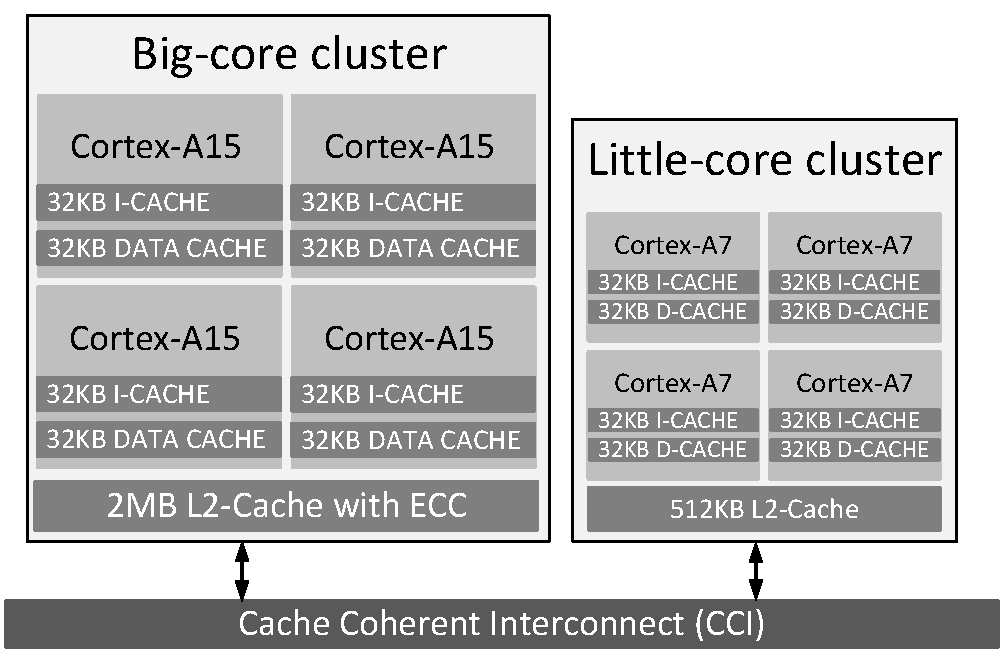
\includegraphics[width=\columnwidth]{figures/block_diagram.pdf}%
        \caption{Samsung Exynos 5422 processor with ARM big.LITTLE architecture.}%
        \label{fig:big-little-diagram}%
        \vspace{-0.56cm}
\end{figure}

In this work, we use of one of the commercially available development boards featuring a big.LITTLE architecture: the Hardkernel Odroid-XU3 development board. As shown in Figure~\ref{fig:big-little-diagram}, the Odroid-XU3 includes an 8-core Samsung Exynos 5422 chip with four ARM Cortex-A15 cores and four Cortex-A7 cores. The four Cortex-A15 share a 2~MB 16-way 64-byte-cache-line L2 cache, while the Cortex-A7 cores share a 512~KB L2 cache. A single memory controller provides access to 2~GB of LPDDR3 RAM with dual 32-bit channels at 1866~MT/s. The reason we use this platform instead of the more up-to-date Juno platform~\cite{Juno} is that even if the latter features the more advanced Cortex~A53 and Cortex~A57 cores, it is limited to six cores instead of the 8 cores in Odroid-XU3.

%Odroid gives us the opportunity to evaluate up to eight cores while Juno, even if it features the more advanced Cortex~A53 and Cortex~A57 cores, is limited to only six total cores. 

The Cortex-A7 cores in this SoC support dual-issue of instructions and their pipeline length is between 8 and 10 stages. The L1 instruction cache is 32KB two-way set associative, with virtually indexed and physically tagged cache-lines that can hold up to 8 instructions. The core supports instruction prefetch by predicting the outcome of branches; the prefetch unit can fetch up to a maximum of four instructions per cycle. The L1 data cache is four-way set associative with physically-indexed and physically-tagged cache lines and uses a pseudo-random replacement policy \cite{TRM_A7}. Dynamic Voltage and Frequency Scaling (DVFS) techniques adjust the frequency of the little cores from 200MHz up to 1.4GHz.

The Cortex-A15 cores in this SoC support triple-issue of instructions and their pipeline length is 
between 15 and 24 stages~\cite{MPR_A15}. The L1 instruction and data caches of the Cortex-A15 are 
both 32~KB and 2-way set-associative with 64~byte cache lines. The processor supports speculative 
instruction execution by maintaining a 2-level global history-based dynamic predictor 
with a branch target buffer~\cite{TRM_A15}. The instruction decode unit performs register renaming 
to remove the Write-After-Write and the Write-After-Read hazards, and promote 
instruction reordering~\cite{TRM_A15}. The instruction dispatch unit analyzes instruction dependences 
before issuing them for execution.  The integer execute unit includes 2 
Arithmetic Logical Units with support for operand forwarding. DVFS techniques vary the 
frequency of the big cores from 200~MHz up to 2~GHz.
For the rest of the paper, we refer to Cortex-A15 cores as \textit{big} and to Cortex-A7 cores as \textit{little}.


%\mm{Explain different pipelines.} \mm{Number of execution units per pipeline?} \mm{ROB size? Maximim number of in-flight instructions?}.  As in the little cores, the data and instruction L1 caches are 32KB each. \mm{FLOPS single and double precision?}.

%In the big.LITTLE processor, the four Cortex-A15 cores form a \emph{cluster} with a shared L2 cache (16-way set-associative with 64 bytes line size), while the Cortex-A7 form a second cluster with a smaller shared L2 cache (8-way 64 bytes cache-line size). This asymmetric multi-core implements the ARMv7 instruction set architecture on all the cores. The two clusters are coherent, so a single shared memory application can run on both clusters, using up to eight cores simultaneously. For the cluster-to-cluster communication, the processor features a cache coherent interconnect. This mechanism allows big and little cores to exchange data at low cost as if they were effectively in the same cluster. Figure~\ref{fig:big-little-diagram} shows a block diagram of such processor.




%%%%%%%%%%%%%%%%%%%
%%%%%%%%%%%%%%%%%%%
% \subsection{Challenges in Scheduling}
% 
% Scheduling a set of processes on an asymmetric multi-core system with big.LITTLE architecture is trickier than the traditional process scheduling on homogeneous multi-cores. 
% An efficient OS scheduler has to take into account the different characteristics of the core types of the system.
% ARM supports two different approaches on scheduling chips with big.LITTLE architecture: the \textit{cluster switching}, and the \textit{global task scheduling}. In this paper we evaluate a different approach which is the \textit{dynamic runtime scheduling} and is not currently used by industry for scheduling such systems. The following subsections describe these different approaches.
% 
% \subsubsection{Cluster Switching}
% In the cluster switching (CS) approach the cores are grouped into two clusters:
% the big-core cluster, that consists of the Cortex-A15 cores of the system and the 
% little-core cluster that consists of the Cortex-A7 cores. 
% At each given time, only one of the clusters is activated; the activated cluster is the one responsible for the execution of the tasks. 
% Thus, the linux OS scheduler does not require any modification and is operating on 4 homogeneous cores each time namely, 
% the cores of the current activated cluster.
% %The deactivated cluster is not processing any task.
% The entire workload of tasks is being managed as a unique entity and the operating system is keeping track of its operational intensity. 
% If the workload reaches a pre-defined threshold, then the entire workload is moved to the other cluster, 
% and the current cluster gets deactivated. 
% %So, the entire workload of tasks is being managed as a unique entity and according to 
% %its operational intensity the OS chooses the appropriate cluster for execution.
% The cluster switching is performed by the CPU frequency framework.
% 
% \subsubsection{Global Task Scheduling (GTS)}
% The second approach is the one that we evaluate in this paper. 
% With the global task scheduling (GTS), all cores are available and visible to the OS scheduler. 
% The OS scheduler is aware of the characteristics and the type of each one of the cores. 
% Moreover, the workload is being managed as a set of tasks, which are practically threads. 
% Each task is characterized by its intensity.
% The OS linux scheduler is modified so that it schedules the high intensity tasks to the big cores (A15 cores)
% and the low intensity tasks to the little cores (A7 cores). 
% This way, the activated cores are chosen according to the tasks of the workload. 
% This is characterized as the most sophisticated method of scheduling tasks on big.LITTLE \cite{samsung}.
% 
% The key benefits of GTS over CS are:
% \begin{itemize}
%  \item Tasks are directly migrated to cores instead of workload being migrated to clusters. This makes the scheduling more flexible and helps on the more effective utilization of the system according to the workload.
% % \item Finer grained control of workloads that are migrated between cores. Because the scheduler is directly migrating tasks between cores, kernel overhead is reduced and power savings can be correspondingly increased.
%  \item Implementation in the scheduler also makes switching decisions faster than in the cpufreq framework, and ARM have reported around 10\% improvements in performance/watt over CS on a range of benchmarks. Samsung reported 20\% improvement in performance.
%  \item GTS can easily support non-symmetrical SoCs (e.g. with 2 Cortex-A15 cores and 4 Cortex-A7 cores)
%  \item The ability to use all cores simultaneously to provide improved peak performance throughput of the SoC compared to CS.
% \end{itemize}
% 
% 
% 
% %Also, interesting slides: http://events.linuxfoundation.org/ sites/events/files/slides/GTS\_Anderson.pdf
% 
% %%%%%%%%%%%%%%%%%%%%%%%%%%%%%%%%%%%%%%%%%%
% %%%%%%%%%%%%%%%%%%%%%%%%%%%%%%%%%%%%%%%%%%
% 
% \subsubsection{Dynamic Scheduling at Runtime Level (task-based)}
% The use of parallel programming models on such systems could increase performance and energy efficiency.
% The increased task granularity that the runtime system can offer has a positive effect on their most effective execution with the minimum possible energy consumption.
% To evaluate this approach we use the OmpSs programming model.
% 
% \textit{OmpSs Programming Model:  }
% OmpSs~\cite{OmpSs} is a task-based programming model conceived as a forerunner of OpenMP. 
% While both OmpSs and OpenMP 4.0 allow the programmers to express tasks and data-dependences between them, OmpSs provides some extra feaatures like runtime support for NUMA-aware allocation or task priorities. 
% OmpSs conceives the parallel execution as a graph where the nodes are sequential pieces of code, the tasks, and the edges are control or data dependences between them.
% 
% The OmpSs runtime is Nanos++, which provides device support for heterogeneity and includes different plug-ins for implementations of scheduling policies, throttling policies, thread barriers, dependency tracking mechanisms, work-sharing and instrumentation. 
% This design allows to maintain the runtime features by adding or removing plug-ins. Thus, the implementation of a new scheduler, or the support of a new architecture becomes simple.
% The implementations of the different scheduling policies in Nanos++ perform various actions on the states of the tasks. A task is \textit{created} if a call to this task is discovered but it is waiting until all its inputs are produced by other previous tasks. When all the input dependencies are satisfied, the task becomes \textit{ready}. The ready tasks of the application at a given point in time are inserted in the \textit{ready queues} as stated by the scheduling policy. Ready queues can be thread-private or shared among multiple threads. When a thread becomes idle, the scheduling policy picks a task from the ready queues for that thread to execute. 
% 
% %\kc{Adding description of fifo scheduler:}
% The default OmpSs scheduling policy is processing the tasks in a first-come first-served manner (FIFO). 
% It maintains a single ready FIFO queue shared among threads for keeping the ready tasks. 
% Whenever a task becomes ready it is pushed to the tail of the ready queue;
% the first available processor, pops the ready task that resides at the head of the ready queue. 
% Simultaneous pushes and pops are protected by the OmpSs locking mechanisms.
% Because the tasks are scheduled dynamically to the available cores, this scheduler achieves automatic load balance without the need of work stealing. 
% Finally, the scheduler is not aware of the task intensity or the core type and its characteristics, but only relies on the availability of tasks and resources.

\iffalse
\mm{Describe only FIFO. In my opinion, extending the evaluation to CATS should be done in an extension paper for a journal.}

Maybe:
\begin{itemize}
 \item Asymmetric Multicores? HW support (Onur Mutlu's ISCAs).
 \item Current processors -- big.LITTLE. Synergistic cores -- Cell.
 \item Other heterogeneous systems: CPU+GPUs, KNL, other accelerators.
\end{itemize}

Hardware support for identifying the most likely critical code segments of parallel applications has been explored. BIC~\cite{Joao:ASPLOS2012} proposes hardware-based tracking of \emph{thread waiting cycles} in parallel regions for bottleneck identification. 
UBA~\cite{Joao:ISCA2013} provides a comprehensive approach for both lagging threads and bottlenecks.


\textbf{Symbiotic cores.}
The ambition of the heterogeneous architecture studies following the nature model of symbiotic relationships
(e.g. water buffalos and birds) is a good approach to optimize overall efficiency of a system. The idea is that
a bunch of less performant cores can take care of a few very performant cores, feeding them with a large
throughput oriented load, minimizing the need to distract their attention to other bookkeeping activities. The
ambition of the project is find out what is the proper dimensioning of such a symbiotic in the development of
highly efficient HPC platforms.

\textbf{From MB3 proposal.}
One of the most widespread approaches to energy efficiency is the use of different computing elements in the
same system. In this task, in particular, we will explore the use of different types of computing cores in an
SoC following a co-design approach between the runtime and architecture. The focus will be on exploring a
symbiotic relationship between small and large cores:

\begin{itemize}
 \item Small cores: Not thought of as the source of computing capacity based on using a large number of
them, but rather seen as support of independent control flows to generate throughput without
perturbing the large/powerful cores, by synchronously executing functions of the runtime that can be
taken out of the critical path and carrying out non-compute bound tasks consuming little power. The
aim is to maximise the efficiency of large cores.

  \item Large cores: Perform bulk of computation task and provide the raw computing power, being
“served” by the small cores. Different variants of the powerful cores will be considered. A first class
of such powerful cores to be considered is the ongoing implementations of the ARM architecture by
multiple companies targeting high performance mobile computing (game-/computer vision-targeted
devices), servers and high capacity systems.

\end{itemize}

We will evaluate different architectural configurations looking at how to integrate large and small cores and
how the runtime can take benefit of such a configuration. We will use the models developed in T5.1 for
conducting actual performance estimation of various architectural configurations. Some of the power models
will also be embedded at this level so as to perform comparative power efficiency assessment of various
configurations.
\fi



%%%%%%%%%%%%%%%%%%%
%%%%%%%%%%%%%%%%%%%
\section{Scheduling in Asymmetric Multi-Cores}
\label{sec:scheduling}
%%%%%%%%%%%%%%%%%%%%%%%%%%%%%%%%%%%%%%%%%%
%%%%%%%%%%%%%%%%%%%%%%%%%%%%%%%%%%%%%%%%%%
Scheduling a set of processes on an AMC system is more challenging than the traditional process scheduling on SMCs. 
An efficient OS scheduler has to take into account the different characteristics of the cores and act accordingly~\cite{coolingAware}.
There have been three mainstream OS schedulers for ARM big.LITTLE systems: \textit{cluster switching}, 
\textit{in-kernel switch} and \textit{global task scheduling}, described in the next sections.
In the case of parallel applications, \textit{dynamic scheduling at the runtime system level} can be exploited to balance the workload among the different cores and is described in section~\ref{sec:runtime}.


%%%%%%%%%%%%%%%%%%%%%%%%%%%%%%%%%%%%%%%%%%
\subsection{Cluster Switching and In-Kernel Switch}
%%%%%%%%%%%%%%%%%%%%%%%%%%%%%%%%%%%%%%%%%%
In the Cluster Switching (CS) approach~\cite{samsung}, only one of the clusters is active at any given time: either the cluster with little cores or the cluster with big cores executes. Thus, the OS scheduler operates on a \emph{de-facto} symmetric multi-core with only four cores, namely the cores of the current active cluster. The policy to change the operating cluster is based on CPU utilization. When idle, background processes are executed on the little cores. When CPU utilization surpasses a threshold, all processes (foreground and background) are migrated to the big cluster. When running on the big cluster, if CPU utilization decreases below a given lower threshold, the entire workload is moved to the little cluster. 
%In this approach, all L2 cache contents are moved from one cluster to the other via the cache coherent interconnect.
%So, the entire workload of tasks is being managed as a unique entity and according to 
%its operational intensity the OS chooses the appropriate cluster for execution.
%An enhanced version of the \texttt{cpufreq} driver, which is driven by CPU utilization, makes the decision to transition from one cluster to the other without involving changes at the OS kernel level.

%%%%%%%%%%%%%%%%%%%%%%%%%%%%%%%%%%%%%%%%%%
% \subsection{In-Kernel Switch}
%%%%%%%%%%%%%%%%%%%%%%%%%%%%%%%%%%%%%%%%%%
In the In-Kernel Switch (IKS) approach~\cite{IKS}, each little core is paired with a big core and it is seen as a single core. On idle, background processes are run on little cores. When the CPU utilization on a given little core surpasses a threshold, the execution on that core is migrated to the big core. When the CPU utilization decreases on that big core below a given threshold, the execution migrates to the associated little core. Thus, at the same time, little and big cores may co-execute, but only one of each pair is active at a given point in time, effectively exploiting just half of the cores concurrently. For both CS and IKS, an enhanced \texttt{cpufreq} driver manages the switching within each core pair.

%The advantage of IKS over CS is that different types of cores can be used at the same time to more efficiently execute a mix of high and low CPU utilization processes. The drawback is that, unlike in CS, the system must have the same number of little and big cores, as they must be paired one to one.


%%%%%%%%%%%%%%%%%%%%%%%%%%%%%%%%%%%%%%%%%%
\subsection{Global Task Scheduling}

%%%%%%%%%%%%%%%%%%%%%%%%%%%%%%%%%%%%%%%%%%
The Global Task Scheduling (GTS)~\cite{samsung}
%\footnote{Different implementations of GTS exist based on the same concepts. Samsung denotes its proprietary implementation \emph{Heterogeneous Multi-Processing}} 
allows running applications on all cores in the asymmetric multi-core. In GTS, all cores are 
available and visible to the OS scheduler, and this scheduler is aware of the characteristics of 
the core types. Each process is assigned to a core type depending on its CPU utilization:
high CPU utilization processes are scheduled to big cores and low CPU utilization processes to 
little cores. GTS also migrates processes between big and little cores when their CPU utilization 
changes. As a result, cores are active depending on the characteristics of the workload. 

The key benefit of GTS is that it can use all the cores simultaneously, providing higher peak 
performance and more flexibility to manage the workload. In GTS tasks are directly migrated to cores 
without needing the intervention of the \texttt{cpufreq} daemon, reducing response time and 
minimizing the overhead of context switches. As a consequence, Samsung reported 20\% improvement in 
performance over CS for mobile benchmarks~\cite{samsung}. Also, GTS supports clusters with 
different number of cores (e.g. with 2 big cores and 4 little cores), while IKS requires to have 
the same number of cores per cluster.

% \begin{itemize}
%  \item In GTS tasks are directly migrated to cores, while in CS the entire workload is migrated to clusters. This makes the scheduling more flexible and helps on the more effective utilization of the system according to the workload.
% % \item Finer grained control of workloads that are migrated between cores. Because the scheduler is directly migrating tasks between cores, kernel overhead is reduced and power savings can be correspondingly increased.
%  %\item Since GTS is implemented in the OS scheduler instead of the \texttt{cpufreq} framework, switching decisions are boosted by 10\% according to ARM~\cite{HEXUS}. Also, 
%  \item GTS can support clusters with different number of cores (e.g. with 2 big cores and 4 little cores), while IKS requires to have exactly the same number of cores per cluster.
%  \item The ability to use all cores simultaneously provides higher peak performance and more flexibility to manage the workload.
% \end{itemize}
% As a result of these characteristics, 
% %ARM reported around 10\% improvements in performance/watt over CS for mobile benchmarks~\cite{}, while 
% Samsung reported 20\% improvement in performance over CS for mobile benchmarks~\cite{samsung}. 
% %\mm{Benefits because of faster transitions, more cores are used or a combination of both?}


%Also, interesting slides: http://events.linuxfoundation.org/ sites/events/files/slides/GTS\_Anderson.pdf

%%%%%%%%%%%%%%%%%%%%%%%%%%%%%%%%%%%%%%%%%%
\subsection{Dynamic Scheduling in the Runtime}
\label{sec:runtime}
%%%%%%%%%%%%%%%%%%%%%%%%%%%%%%%%%%%%%%%%%%
%In the context of parallel applications, the OS lacks knowledge about their internal structure and CPU utilization may be ineffective to schedule its threads (seen as processes in Linux). The runtime system of the parallel programming model has this knowledge and therefore seems to be the right entity in the software stack to perform the application scheduling to exploit multi-core asymmetry for better performance and energy efficiency.


%The use of parallel programming models on such systems could increase performance and energy efficiency. 
Current programming models for shared memory systems such as OpenMP rely on a 
runtime system to manage the execution of the parallel application. 
In this work, we make use of two types of programming models: loop- and task-based.
Loop-based scheduling distributes the iterations of a loop among the 
threads available in the system, following a traditional \textit{fork-join} model.
OpenMP supports loop-based scheduling through its \emph{parallel for} directives. 
This clause implies a barrier synchronization at the end of the loop\footnote{unless 
specified otherwise with the \texttt{nowait} clause}, and supports either static or dynamic loop 
scheduling. 

With static loop scheduling, the iterations of a loop are divided to as many chunks as the number of cores.
Then, every core executes the assigned chunk, leading to a low-overhead static scheduling.
% that even the compiler can generate code for it without the need of runtime intervention.
In addition, OpenMP supports dynamic loop scheduling. 
It generates more chunks than cores, and assigns them to the available cores at runtime. 
This is more suitable to asymmetric multi-core systems where the cores are not similar and a static iteration assignment would cause load imbalance.
%To evaluate this approach we use the OpenMP programming model.

Recent advances in programming models recover the use of task-based programming models to simplify parallel programming of multi-cores~\cite{OpenMP4.0:Manual2013, OmpSs_PPL11, Zuckerman:EXADAPT2011, Bauer.2012.SC, Vandierendonck:PACT2011}. 
In these models the programmer splits the code in sequential pieces of work (tasks) and specifies the data dependencies among them.  
With this information the runtime system schedules tasks and manages synchronization. These models ease programmability~\cite{OpenMP4.0:Manual2013, OmpSs_PPL11, Zuckerman:EXADAPT2011, Bauer.2012.SC, Vandierendonck:PACT2011, Vandierendonck:Hyperq},
%~\cite{clusterss,clusterss_cpe}, 
and also increase performance by avoiding global synchronization points.
%The increased task granularity that the runtime system can offer has a positive effect on their most effective execution with the minimum possible energy consumption.

%\textit{OmpSs Programming Model:}
% To evaluate this approach we use OmpSs~\cite{OmpSs_PPL11}, a task-based programming model conceived as a forerunner of OpenMP~\cite{OpenMP4.0:Manual2013}. 
To evaluate this approach we make use of OpenMP tasking support~\cite{OpenMP4.0:Manual2013}. 
OpenMP allows expressing tasks and data dependences between them using equivalent code annotations. 
It conceives the parallel execution as a \emph{task dependence graph} (TDG), where nodes are 
sequential pieces of code (tasks) and the edges are control or data dependences between them. 
The runtime system builds this TDG at execution time and dynamically schedules tasks to the available cores.
Tasks become ready as soon as their input dependencies are satisfied.
The scheduling of the ready tasks is done in a first-come-first-served manner, using a FIFO scheduler.  
Even though this scheduler is not aware of the task computational requirements or the core type and its performance and power characteristics, it can balance the load as long as there are ready tasks available thanks to the lack of global synchronization.


%\kc{maybe we should remove these details? We do not include such details for loop scheduling}A task is \textit{created} when a call to this task is discovered in the code. The runtime system adds it to the TDG using the specified input dependences. The task cannot be scheduled until all its inputs dependences are produced by other tasks previously created. When all dependences are satisfied, the task becomes \textit{ready} and is inserted in a \textit{ready queue}. At this point, the task can be executed according to the scheduling policy of the runtime. Ready queues can be thread-private or shared among multiple threads. When a thread becomes idle, the scheduling policy selects a task from a ready queue and it is executed in that particular thread.

%\kc{do we need to explain the fifo scheduler? }%\kc{Adding description of fifo scheduler:}
%The default scheduling policy is processing the tasks in a \emph{first in, first out} manner (FIFO). 
%This policy is implemented with a single ready FIFO queue shared among all threads for keeping the ready tasks. 
%Whenever a task becomes ready it is pushed to the tail of the ready queue;
%the first available processor, pops the ready task that resides at the head of the ready queue. 
%Simultaneous pushes and pops are protected by locking mechanisms.
%Because tasks are scheduled dynamically to available cores, this scheduler automatically balances the load without the need of work stealing. This FIFO scheduler is not aware of the task computational requirements or the core type and its performance and power characteristics, but only relies on the availability of tasks and resources.

%More advanced runtime features are also available, providing runtime support for NUMA-aware allocation, task priorities, device support for heterogeneity, different scheduling policies, throttling policies, dependence tracking mechanisms, work-sharing and work stealing. However, in this paper we make use of the simple FIFO scheduler and the vanilla features of the runtime system for a fair comparison with GTS.



% \subsection{Dynamic Scheduling at Operating System Level}
% 
% Scheduling a set of processes on an asymmetric multi-core system with big.LITTLE 
% architecture is trickier than the traditional process scheduling on 
% homogeneous multi-cores. An efficient OS scheduler has to take into account
% the different characteristics of the core types of the system.
% ARM supports two different approaches on scheduling chips with big.LITTLE architecture:
% the \textit{cluster switching}, and the \textit{global task scheduling}. 
% 
% In the cluster switching (CS) approach the cores are grouped into two clusters:
% the big-core cluster, that consists of the Cortex-A15 cores of the system and the 
% little-core cluster that consists of the Cortex-A7 cores. 
% At each given time, only one of the clusters is activated; the activated cluster is the one responsible for the execution of the tasks. 
% Thus, the linux OS scheduler does not require any modification and is operating on 4 homogeneous cores each time namely, 
% the cores of the current activated cluster.
% %The deactivated cluster is not processing any task.
% The entire workload of tasks is being managed as a unique entity and the operating system is keeping track of its operational intensity. 
% If the workload reaches a pre-defined threshold, then the entire workload is moved to the other cluster, 
% and the current cluster gets deactivated. 
% %So, the entire workload of tasks is being managed as a unique entity and according to 
% %its operational intensity the OS chooses the appropriate cluster for execution.
% The cluster switching is performed by the CPU frequency framework.
% 
% 
% The second approach is the one that we evaluate in this paper. 
% With the global task scheduling (GTS), all cores are available and visible to the OS scheduler. 
% The OS scheduler is aware of the characteristics and the type of each one of the cores. 
% Moreover, the workload is being managed as a set of tasks, which are practically threads. 
% Each task is characterized by its intensity.
% The OS linux scheduler is modified so that it schedules the high intensity tasks to the big cores (A15 cores)
% and the low intensity tasks to the little cores (A7 cores). 
% This way, the activated cores are chosen according to the tasks of the workload. 
% This is characterized as the most sophisticated method of scheduling tasks on big.LITTLE \cite{samsung}.
% 
% The key benefits of GTS over CS are:
% \begin{itemize}
%  \item Tasks are directly migrated to cores instead of workload being migrated to clusters. This makes the scheduling more flexible and helps on the more effective utilization of the system according to the workload.
% % \item Finer grained control of workloads that are migrated between cores. Because the scheduler is directly migrating tasks between cores, kernel overhead is reduced and power savings can be correspondingly increased.
%  \item Implementation in the scheduler also makes switching decisions faster than in the cpufreq framework, and ARM have reported around 10\% improvements in performance/watt over CS on a range of benchmarks. Samsung reported 20\% improvement in performance.
%  \item GTS can easily support non-symmetrical SoCs (e.g. with 2 Cortex-A15 cores and 4 Cortex-A7 cores)
%  \item The ability to use all cores simultaneously to provide improved peak performance throughput of the SoC compared to IKS.
% \end{itemize}
% 
% 
% 
% %Describe OS process scheduler developed by ARM for the big.LITTLE.
% 
% %GNU/Linux based, Ubuntu 14.04 LTS
% 
% %Vanilla Linux kernel with an additional scheduler. Developed by ARM for their big.LITTLE platform: the Global Task Scheduler
% 
% %Assigns processes/threads to slow or big cores based on the load the process generates
% 
% %An upper and lower threshold, average load to decide when to move from one cluster of cores to the other.
% 
% %From: https://www.linaro.org/blog/hardware-update/big-little-software-update/
% 
% %The second is the Global Task Scheduling (GTS) software developed (and now named) by ARM. This is known in Linaro as big.LITTLE MP. Using GTS all of the big and LITTLE cores are available to the Linux kernel for scheduling tasks. We are very proud that Linaro has contributed to ARM’s development of the GTS software, and that it is now publicly available in Linaro builds. ARM and Linaro recommend GTS for new products, and Linaro members are actively planning product deployments using this solution.
% 
% %Core Software Configuration for GTS (4+4)
% 
% 
% %The key benefits of GTS over IKS are:
% 
% %\begin{itemize}
% % \item Finer grained control of workloads that are migrated between cores. Because the scheduler is directly migrating tasks between cores, kernel overhead is reduced and power savings can be correspondingly increased.
% % \item Implementation in the scheduler also makes switching decisions faster than in the cpufreq framework, and ARM have reported around 10\% improvements in performance/watt over IKS on a range of benchmarks.
% % \item The ability to easily support non-symmetrical SoCs (e.g. with 2 Cortex-A15 cores and 4 Cortex-A7 cores)
% % \item The ability to use all cores simultaneously to provide improved peak performance throughput of the SoC compared to IKS.
% 
% %\end{itemize}
% 
% %The big.LITTLE MP patch set creates a list of Cortex-A15 and Cortex-A7 cores that is used to pick the target core for a particular task. Then, using runnable load average statistics, the Linux scheduler is modified to track the average load of each task, and to migrate tasks to the best core. High intensity tasks are migrated to the Cortex-A15 core(s) and are also marked as high intensity tasks for more efficient future allocations.  Low intensity tasks remain resident on the Cortex-A7 core(s).
% 
% %Also, interesting slides: http://events.linuxfoundation.org/ sites/events/files/slides/GTS\_Anderson.pdf
% 
% %%%%%%%%%%%%%%%%%%%%%%%%%%%%%%%%%%%%%%%%%%
% %%%%%%%%%%%%%%%%%%%%%%%%%%%%%%%%%%%%%%%%%%
% \subsection{Dynamic Scheduling at Runtime Level}
% 
% \subsubsection{OmpSs Programming Model}
% %OmpSs is a task-based programming model that offers a high level abstraction to the implementation of parallel applications for various homogeneous and heterogeneous architectures~\cite{OmpSs_PPL11,OmpSs}. It enables the annotation of function declarations with the task directive, which declares a task. Every invocation of a such function creates a task that is executed concurrently with other tasks or parallel loops. OmpSs also supports task dependencies and it uses the StarSs~\cite{StarSs} dependency tracking mechanisms. OmpSs is built with the support of the Mercurium compiler, responsible for the translation of the OmpSs annotation clauses to source code, and the Nanos++ runtime system, responsible for the internal creation and execution of the tasks.
% 
% %As a task-based parallel programming model, OmpSs enables the annotation of function declarations with the task directive. If a function is declared as a task, then every invocation of this function creates a task that is executed concurrently with other tasks or parallel loops. The accessible data to each task are the arguments of the function. OmpSs uses the StarSs~\cite{StarSs} dependency tracking mechanisms and each task may be annotated with the \textit{in}, \textit{out}, \textit{inout} clauses. These clauses allow the specification of scalars, arrays and pointers as input, output or input and output data of a task. The implementation of a barrier is supported under the \textit{taskwait} clause, and it can also be used with the addition of the \textit{on} clause, to declare a barrier for the group of tasks that produce a specific piece of data. These original OmpSs features can now be found in OpenMP 4.0~\cite{OpenMP}.
% 
% OmpSs~\cite{OmpSs} is a task-based programming model conceived as a forerunner of OpenMP. 
% While both OmpSs and OpenMP 4.0 allow the programmers to express tasks and data-dependences between them, OmpSs provides some extra feaatures like runtime support for NUMA-aware allocation or task priorities. 
% OmpSs conceives the parallel execution as a graph where the nodes are sequential pieces of code, the tasks, and the edges are control or data dependences between them.
% 
% The OmpSs runtime is Nanos++, which provides device support for heterogeneity and includes different plug-ins for implementations of scheduling policies, throttling policies, thread barriers, dependency tracking mechanisms, work-sharing and instrumentation. 
% This design allows to maintain the runtime features by adding or removing plug-ins. Thus, the implementation of a new scheduler, or the support of a new architecture becomes simple.
% The implementations of the different scheduling policies in Nanos++ perform various actions on the states of the tasks. A task is \textit{created} if a call to this task is discovered but it is waiting until all its inputs are produced by other previous tasks. When all the input dependencies are satisfied, the task becomes \textit{ready}. The ready tasks of the application at a given point in time are inserted in the \textit{ready queues} as stated by the scheduling policy. Ready queues can be thread-private or shared among multiple threads. When a thread becomes idle, the scheduling policy picks a task from the ready queues for that thread to execute. 
% 
% \kc{The task priorities do not need to be described in my opinion}
% The Nanos++ internal data structures support task prioritization. The task priority is an integer field inside the task descriptor that rates the importance of the task. If the scheduling policy supports priorities, the ready queues are implemented as \textit{priority queues}. In a priority queue, tasks are sorted in a decreasing order of their priority. The insertion in a priority queue is always ordered and the removal of a task is always from the head of the queue, i.e., the task with the highest priority. The priority of a task can be either set in user code, by using the \textit{priority} clause, which accepts an integer priority value or expression, or dynamically  by the scheduling policy, as is described in the next section.
% 
% \kc{Adding description of fifo scheduler:}
% The default OmpSs scheduling policy is processing the tasks in a first-come first-served manner (FIFO). 
% It maintains a single ready FIFO queue shared among threads for keeping the ready tasks. 
% Whenever a task becomes ready it is pushed to the tail of the ready queue;
% the first available processor, pops the ready task that resides at the head of the ready queue. 
% Simultaneous pushes and pops are protected by the OmpSs locking mechanisms.
% Because the tasks are scheduled dynamically to the available cores, this scheduler achieves automatic load balance without the need of work stealing. 
% Finally, the scheduler is not aware of the task intensity or the core type and its characteristics, but only relies on the availability of tasks and resources.
% 
% 
% \mm{Describe only FIFO. In my opinion, extending the evaluation to CATS should be done in an extension paper for a journal.}


%%%%%%%%%%%%%%%%%%%
%%%%%%%%%%%%%%%%%%%
\section{Experimental Methodology}
\label{sec:experimental}
%\begin{table*}[!t]
%	\centering
%	\scriptsize
%	\caption{Benchmarks used from the PARSEC benchmark suite and their 
%measured performance ratio between big and little cores}
%    %\vspace{-0.2cm}
%	\setlength{\tabcolsep}{3pt}
%	\begin{tabular}{|p{2cm}|p{4.7cm}|p{2.5cm}|c|c|}
%	\hline
%	\textbf{Benchmark} & \multicolumn{1}{|c|}{\textbf{Description}} & \multicolumn{1}{|c|}{\textbf{Input}} & \textbf{Parallelization} & \multicolumn{1}{|c|}{\textbf{Perf ratio}} \\
%	\hline \hline
%	blackscholes & Calculates the prices of a portfolio analytically with the Black-Scholes partial differential equation. & 10,000,000 options & data-parallel &2.18 \\ \hline
%	bodytrack & Computer vision application which tracks a 3D pose of a marker-less human body with multiple cameras through an image sequence. & 4 cameras, 261 frames, 4,000 particles, 5 annealing layers & pipeline & 4.16 \\ \hline
%	canneal & Simulated cache-aware annealing to optimize routing cost of a chip design. & 2.5 million elements, 6,000 steps & unstructured & 1.73 \\ \hline
%	dedup & Compresses a data stream with a combination of global compression and local compression in order to achieve high compression ratios. & 351 MB data & pipeline & 2.67 \\ \hline
%	facesim & Takes a model of a human face and a time sequence of muscle activation and computes a visually realistic animation of the modeled face. & 100 frames, 372,126 tetrahedra & data-parallel & 3.40 \\ \hline
%	ferret & Content-based similarity search of feature-rich data (audio, images, video, etc.) & 3,500 queries, 59,695 images database, find top 50 images & pipeline & 3.59 \\ \hline
%	fluidanimate & Extended Smoothed Particle Hydrodynamics method to simulate an 
%incompressible fluid for interactive animations. & 500 frames, 500,000 particles & 
%data-parallel & 3.32 \\ \hline
%%	freqmine & Intel RMS application which employs an array-based version of the FP-growth (Frequent Pattern-growth) method for Frequent Itemset Mining (FIMI). & 250,000 HTML documents, minimum support 11,000 & 2,231\\ \hline
%%	raytrace & Intel RMS workload which renders an animated 3D scene. & 200 frames, 1,920$\times$1,080 pixels, 10 million polygons & 13,751\\ \hline
%	streamcluster & Solves the online clustering problem. & 200K points per block, 5 block & 
%data-parallel & 3.48 \\ \hline
%	swaptions & Intel RMS workload; uses the Heath-Jarrow-Morton framework to price a portfolio of swaptions. & 128 swaptions, 1 million  simulations & data-parallel & 2.78 \\ \hline
%%	vips & VASARI Image Processing System (VIPS), which includes fundamental image processing operations. & 18,000$\times$18,000 pixels & 127,957\\ \hline
%%	x264 & H.264/AVC (Advanced Video Coding) video encoder. & 512 frames, 1,920$\times$1,080 pixels & 29,329\\ \hline 
%	\end{tabular}
%	\label{tab:parsec}
%	%\vspace{-0.3cm}
%\end{table*}


\begin{table*}[!t]
	\centering
	\scriptsize
	\caption{Benchmarks used from the PARSEC benchmark suite and their 
		measured performance ratio between big and little cores}
	%\vspace{-0.2cm}
	\setlength{\tabcolsep}{3pt}
	\begin{tabular}{|p{2cm}|p{2.5cm}|c|c|}
		\hline
		\textbf{Benchmark} & \multicolumn{1}{|c|}{\textbf{Input}} & \textbf{Parallelization} & \multicolumn{1}{|c|}{\textbf{Perf ratio}} \\
		\hline \hline
		blackscholes & native & data-parallel &2.18 \\ \hline
		bodytrack & native & pipeline & 4.16 \\ \hline
		canneal & native & unstructured & 1.73 \\ \hline
		dedup & 351 MB data & pipeline & 2.67 \\ \hline
		facesim & native & data-parallel & 3.40 \\ \hline
		ferret & native & pipeline & 3.59 \\ \hline
		fluidanimate & native & data-parallel & 3.32 \\ \hline
		streamcluster & native & data-parallel & 3.48 \\ \hline
		swaptions & native & data-parallel & 2.78 \\ \hline
	\end{tabular}
	\label{tab:parsec}
\end{table*}

%%%%%%%%%%%%%%%%%%%%%%%%%%%%%%%%%%%%%%%%%%
%%%%%%%%%%%%%%%%%%%%%%%%%%%%%%%%%%%%%%%%%%
% All the experiments in this paper are performed on the Hardkernel ODROID XU3 described in Section~\ref{sec:background}. In this platform, there are four separated current sensors to measure in real time the power consumption of the cluster of A15 cores, the cluster of A7 cores, the GPU and DRAM.
% 
% We measure the execution time and power of nine applications from the PARSEC benchmark suite~\cite{Bienia:PhD2011}.
% We compare performance and energy of three different scheduling approaches:
% \begin{itemize}
% \item \textit{Static threading}: the OS is not allowed to migrate threads between the clusters of big and little cores. Scheduling decisions are made at the application level.
% \item \textit{GTS}: dynamic coarse-grained OS scheduling with the integrated in the Linux kernel Global Task Scheduler~\cite{samsung, ARM} using the default version of PARSEC benchmarks.
% \item \textit{Task-based}: dynamic fine-grained runtime scheduling with OmpSs programming model using the PARSECSs~\cite{Chasapis:TACO2016} suite for the OmpSs implementations of the applications.
% \end{itemize}



%OmpSs which is representing the \textit{task-based} runtime scheduling approach, the default pthreads version of PARSEC where the  operating system's Global Task Scheduler (GTS) is used for scheduling, and finally, the modified pthreads version that pins the threads on cores, which disables every kind of scheduling on the chip thus enables \textit{static threading}.

%\subsection{Evaluated Platform}

%The Hardkernel ODROID-XU3 development board has an 8-core Samsung Exynos 5422 chip with an ARM big.LITTLE architecture and 2GB of LPDDR3 RAM at 933MHz. The chip has four Cortex-A15 cores at 1.6GHz and four Cortex-A7 cores at 800MHz. The four Cortex-A15 cores form a \textit{cluster} with a shared 2MB L2 cache, and the Cortex-A7 share a 512KB L2 cache. The two \textit{clusters} are coherent, so a single shared memory application can run on both clusters, using up to eight cores simultaneously. In our experiments, we evaluate a set of possible combinations of fast and slow cores varying the total number of cores from four to eight. For the remainder of the paper, we refer to Cortex-A15 cores as \textit{big} and to Cortex-A7 cores as \textit{little}.




%%%%%%%%%%%%%%%%%%%%%%%%%%%%%%%%%%%%%%%%%%
%%%%%%%%%%%%%%%%%%%%%%%%%%%%%%%%%%%%%%%%%%
\subsection{Metrics}
\label{sec:metrics}

All the experiments in this paper are performed on the Hardkernel Odroid XU3 described in Section~\ref{sec:background}. 
\textcolor{blue}{
\textbf{R3Q6: }In our experiments we keep the frequencies of the cores static.
This is in order to first, avoid machine overheating, and second to prevent the DVFS governor to dynamically modify the frequency of the cores during runtime, thing that would affect the reliability of the results.
We make use of the \texttt{cpufreq} driver to set big cores at 1.6GHz and little cores at 800MHz. 
}

%To estimate the impact of the different kinds of cores, 
We evaluate seven configurations with different numbers of \textit{little} (L) and \textit{big} (B) cores, denoted \texttt{L+B}.
For each configuration and benchmark, we report the average performance of five executions in the application parallel region. Then, we report the application speedup over its execution time on one little core.
\textcolor{blue}{\textbf{R3Q7: }The variability of the results among the five runs is very small and the stdev of the speedup obtained ranges from 0 to 1.1, averaging at 0.85.}
Equation~\ref{eq.speedup} shows the formula to compute this speedup.
\begingroup\makeatletter\def\f@size{9}\check@mathfonts
\begin{equation}
  \text{Speedup(L, B, method)} = \frac{\text{Exec. time(1, 0, method)}}{\text{Exec. time(L, B, 
method)}}
\label{eq.speedup}
\end{equation}
\endgroup

%Each set-up has a given number of \textit{little} (L) and \textit{big} (B) cores, denoted (L+B). Each benchmark is run on the target set-up seven times measuring performance, 
%power and energy of the specified region of interest\footnote{The parallel region of the benchmark, which is marked in the distributed codes}. %We select the repetition with the best performance and report all the metrics corresponding to this execution.

In this platform, there are four separated current sensors to measure, in real time, the power consumption of the A15 cluster, the A7 cluster, the GPU and DRAM. 
To gather power and energy measurements, a background daemon reads the machine power 
sensors periodically during the application execution with negligible overhead. 
Sensors are read at their refresh rate, every 270ms, and the values of A7 and A15 clusters' sensors are collected.
%and their values are written in a file. 
With the help of timestamps, we correlate the power measurements with the application parallel region in a \emph{post-mortem} process.
%\footnote{The parallel region duration is several orders of magnitude longer than the reading frequency of power sensors}. 
\textcolor{blue}{
\textbf{R3Q8:} The execution time overhead of the running daemon is measured and verified to be less than 3\%. \footnote{In most cases this overhead is 1\% with some applications reaching 2\%.}
}
The reported power consumption is the average power tracked during five executions of each configuration, considering the application parallel region only. 
We then report average power in Watts along the execution. 

Finally, in terms of energy and Energy Delay Product (EDP), we report the total energy and EDP of 
the benchmarks region of interest.
\textcolor{blue}{
\textbf{R3Q9:} To facilitate the explanation of these results and isolate the impact of the different system configurations on the energy consumption we normalize these results to the run on four little cores with static threading.
}
Equations~\ref{eq.energy} and~\ref{eq.edp} show the formulas for these calculations.
\begingroup\makeatletter\def\f@size{8}\check@mathfonts
\begin{equation}
  \text{Normalized Energy(L, B, method)} = \frac{\text{Energy(L, B, method)}}{\text{Energy(4, 0, static-threading)}}
  \label{eq.energy}
\end{equation}
\begin{equation}
  \text{Normalized EDP(L, B, method)} = \frac{\text{EDP(L, B, method)}}{\text{EDP(4, 0, static-threading)}}
  \label{eq.edp}
\end{equation}
\endgroup




%%%%%%%%%%%%%%%%%%%%%%%%%%%%%%%%%%%%%%%%%%
%%%%%%%%%%%%%%%%%%%%%%%%%%%%%%%%%%%%%%%%%%
\subsection{Applications}
\label{sec:parsec}

With the prevalence of many-core processors and the increasing relevance of application 
domains that do not belong to the traditional HPC field, comes the need for programs 
representative of current and future parallel workloads. 
The PARSEC benchmark suite~\cite{PARSEC3,Bienia:PhD2011} features state-of-the-art, 
computationally intensive algorithms and very diverse workloads from different areas of computing.
In our experiments, we make use of the original PARSEC codes together with a task-based 
implementation of nine benchmarks of the suite~\cite{Chasapis:TACO2016}. 

Table~\ref{tab:parsec} shows the benchmarks included in the study along with their respective 
inputs, parallelization strategy and performance ratio between big and little cores per application. 
We are using native inputs, which are real input sets for native execution, except for \texttt{dedup}, as the entire native input file of 672 MB and the intermediate data structures do not fit in the memory system of our platform. 
Instead, we reduce the size of the input file to 351 MB.

\begin{figure}[t]%
	\centering
	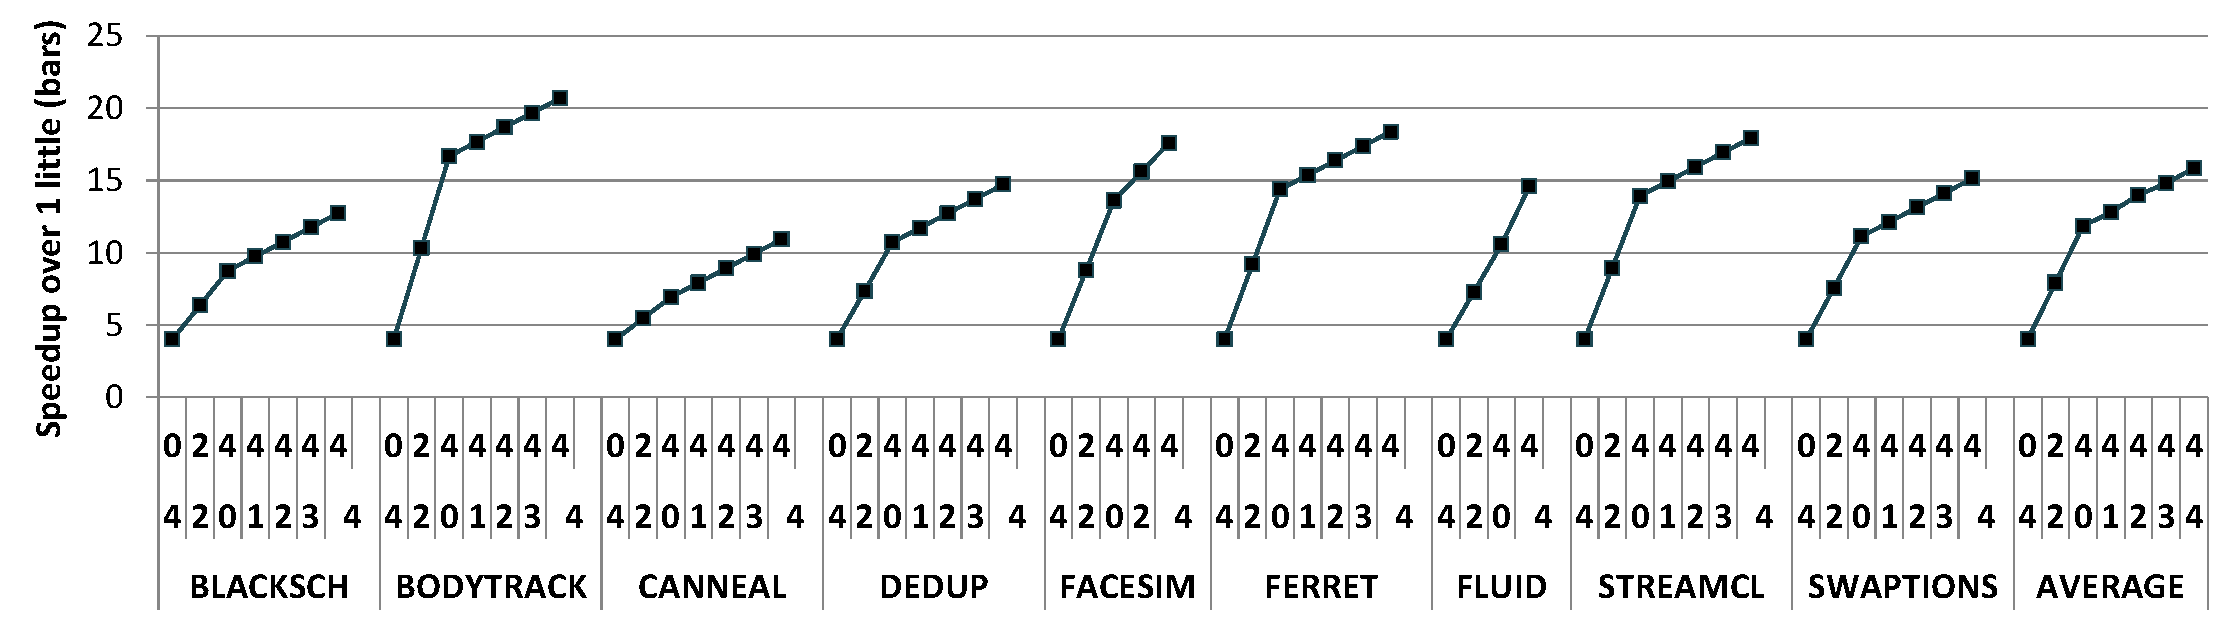
\includegraphics[width=1\columnwidth]{figures/ideal_speedup_new.pdf}
	\caption{Ideal speedup over 1 little core according to Equation~\ref{eq.ideal}. Numbers at the bottom of x axis show the number of little cores, numbers above it show the number of big cores}
	%Results are reported for systems with 0, 2 and 4 big cores, and a total number of cores between 4 and 8.}	
	\label{fig:ideal}%
\end{figure}

The original codes make use of the \texttt{pthreads} parallelization model for all the selected benchmarks. 
The taskified applications follow the same parallelization strategy implemented with OpenMP~4.0 task annotations.
The task-based implementation is done following two basic ideas: i) remove barriers where possible, by adding explicit data-dependencies; and ii) remove application-specific load balancing mechanisms, such as application-specific pools of threads implemented in \texttt{pthreads} and delegate this responsibility to the runtime.
%As a result, both codes achieve the same performance on homogeneous processors with a reduced number of cores~\cite{Chasapis:TACO2016}, while significantly reducing the total number of lines of code for benchmarks with application-specific load balancing mechanisms (bodytrack, dedup and ferret).

%%%%%%%%%%%%%%%%%%%%%%%%%%%%%%%%%%%%%%%%%%
%%%%%%%%%%%%%%%%%%%%%%%%%%%%%%%%%%%%%%%%%%
%\subsection{Performance Ratio Characterization}

When running on the big.LITTLE processor, each benchmark exhibits different performance ratios between big and little cores. These ratios tell us how many times faster a big core is compared to a little core. We measure the performance ratio of each application by executing it first on one big core and then on one little core, which corresponds to Speedup(0, 1, task-based) in Equation~\ref{eq.speedup}. 
% The equation for the performance ratio is the following:
% \begingroup\makeatletter\def\f@size{8}\check@mathfonts
% \begin{equation}
%   \text{Perf\_ratio(workload)} = \frac{\text{Exec. time(workload, 1little)}}{\text{Exec. time(workload, 1big)}}
%   \label{eq.perf_ratio}
% \end{equation}
% \endgroup
Table~\ref{tab:parsec} also includes the observed performance ratio for each application. Bodytrack is the application that benefits the most from running on the big core with a performance ratio of 4.16$\times$. The out-of-order execution of the big core together with an increased number of in-flight instructions significantly improves the performance of this application. In contrast, canneal is the benchmark with the lowest performance ratio, 1.73$\times$, as this is a memory-intensive benchmark that does not benefit as much from the extra computation power of the big core. In general, performance ratios are above 2.5$\times$ for seven out of nine benchmarks, reaching 3.03$\times$ on average. 

% In terms of power, the average ratio is significantly higher, 5$\times$, while the observed values vary between X and Y. \mm{Explain a bit more}.

Taking into account these performance ratios, we can estimate the ideal speedup of the platform for each workload assuming a perfect parallelization strategy. 
\textcolor{blue}{
\textbf{R1Q8:} This metric is useful for understanding the potential of each application irrespective of parallelization strategy and scheduling approach. 
It isolates the computations of each application and shows its ideal performance for each possible confuguration of the AMC.
}
Equation \ref{eq.ideal} shows the equation for the ideal speedup over 1 little core computation according to the number of big (B) and little (L) cores.
\begingroup\makeatletter\def\f@size{8}\check@mathfonts
\begin{equation}
  \text{Ideal speedup(workload, B, L)} = \text{B $\times$ Perf\_ratio(workload) $+$ L}
\label{eq.ideal}
\end{equation}
\endgroup


Figure~\ref{fig:ideal} shows the ideal speedup of the system for each application for the varying numbers of cores. 
This speedup assumes that the applications are fully parallel with no barriers or other synchronization points. 
Thus, these speedups are an upper bound of the achievable application performance.
%As expected, benchmarks with higher performance ratios exhibit potentially higher speed-ups on the asymmetric multi-core.


%%%%%%%%%%%%%%%%%%%
%%%%%%%%%%%%%%%%%%%
\section{Evaluation}
\label{sec:evaluation}

% \mm{We don't need to include Figure~\ref{fig:edp4} as its average results are already in the previous figure.}
% \begin{figure*}[t]%
% 	\centering
% 	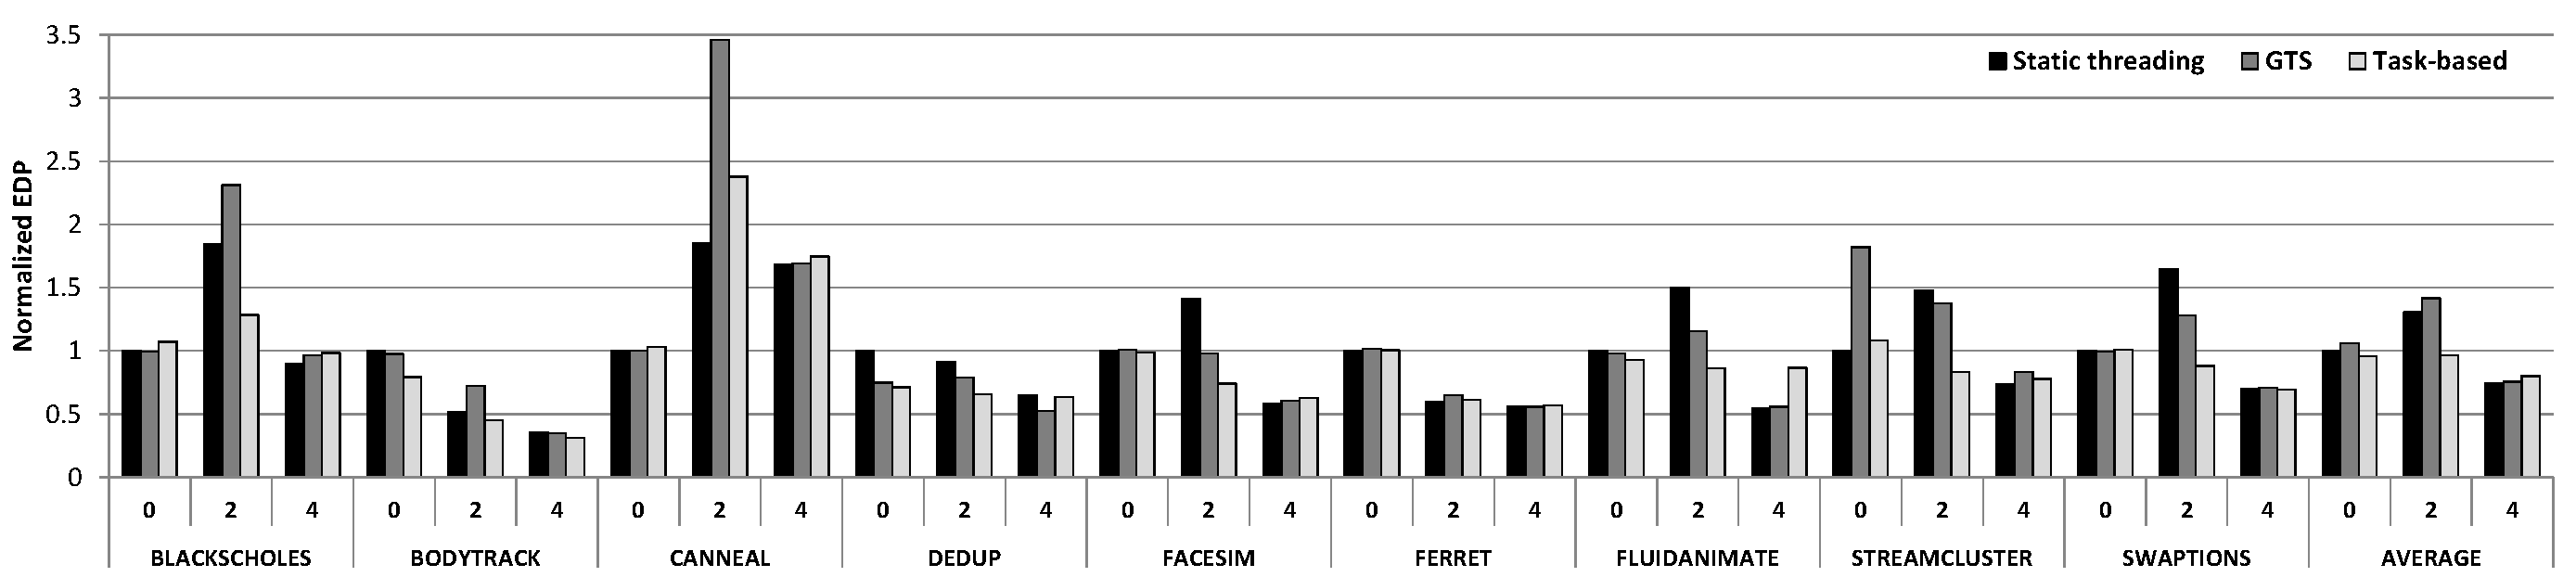
\includegraphics[width=1.0\textwidth]{figures/edp4.pdf}
% 	\vspace{-0.3cm}
% 	\caption{Normalized EDP on a 4-core system with 0, 2, and 4 big cores. Results are normalized with respect to static-threading EDP results with 4 little cores.}
% 	%\caption{Performance improvements on a big.LITTLE processor with different $(F,N)$ configurations, where $F$ is the total number of big cores and $N$ the total number of cores. Results are normalized to running on four little cores with pinned Pthreads.}%
% 	\label{fig:edp4}%
% \end{figure*}


% \begin{figure*}[t]%
% 	\centering
% 	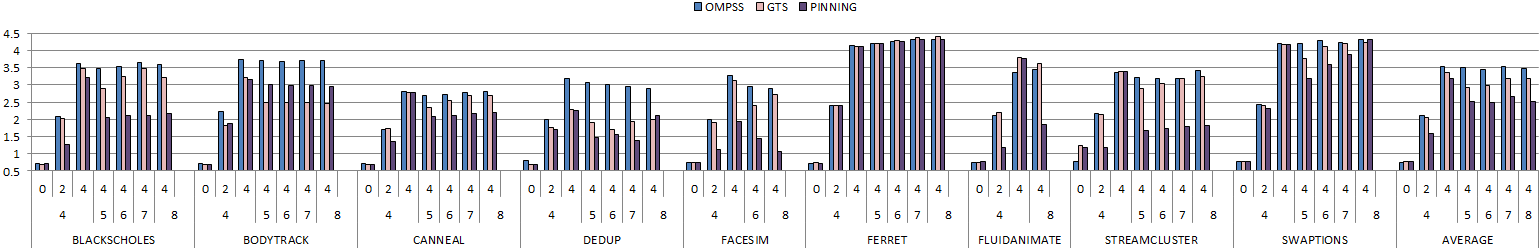
\includegraphics[width=1.0\textwidth]{figures/power-parsec}
% 	\vspace{-0.3cm}
% 	\caption{Average power consumption on a big.LITTLE processor with different $(F,N)$ configurations, where $F$ is the total number of big cores and $N$ the total number of cores.}%
% 	\label{fig:all-power}%
% \end{figure*}
% 
% \begin{figure*}[t]%
% 	\centering
% 	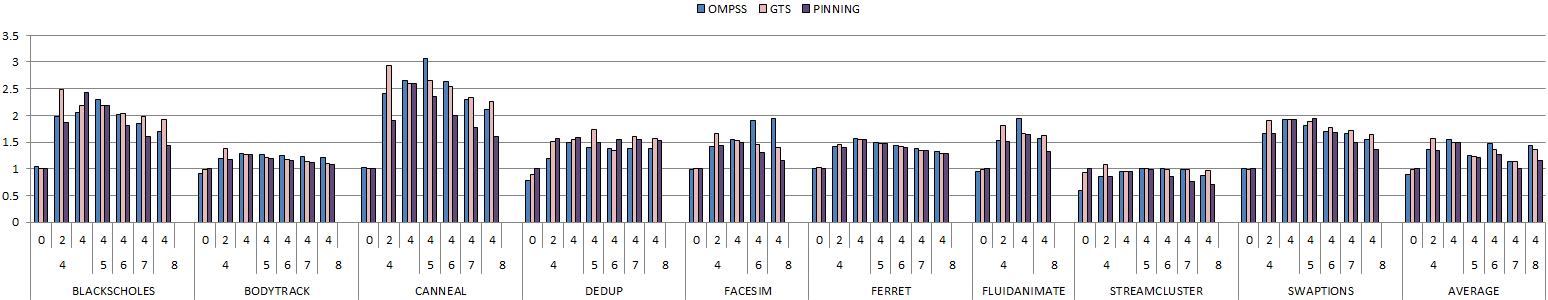
\includegraphics[width=1.0\textwidth]{figures/energy-parsec}%
% 	\vspace{-0.3cm}
% 	\caption{Energy consumption on a big.LITTLE processor with different $(F,N)$ configurations, where $F$ is the total number of big cores and $N$ the total number of cores. Results are normalized to running on four little cores with pinned Pthreads.}%
% 	\label{fig:all-energy}%
% \end{figure*}
% 
% 
% 
% \begin{figure*}[t]%
% 	\centering
% 	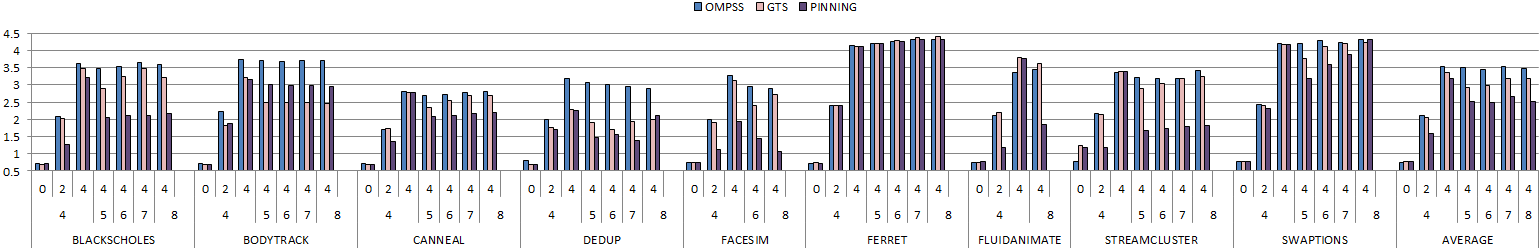
\includegraphics[width=1.0\textwidth]{figures/power-parsec}
% 	\vspace{-0.3cm}
% 	\caption{Average power consumption on a big.LITTLE processor with different $(F,N)$ configurations, where $F$ is the total number of big cores and $N$ the total number of cores.}%
% 	\label{fig:all-power}%
% \end{figure*}
% 
% \begin{figure*}[t]%
% 	\centering
% 	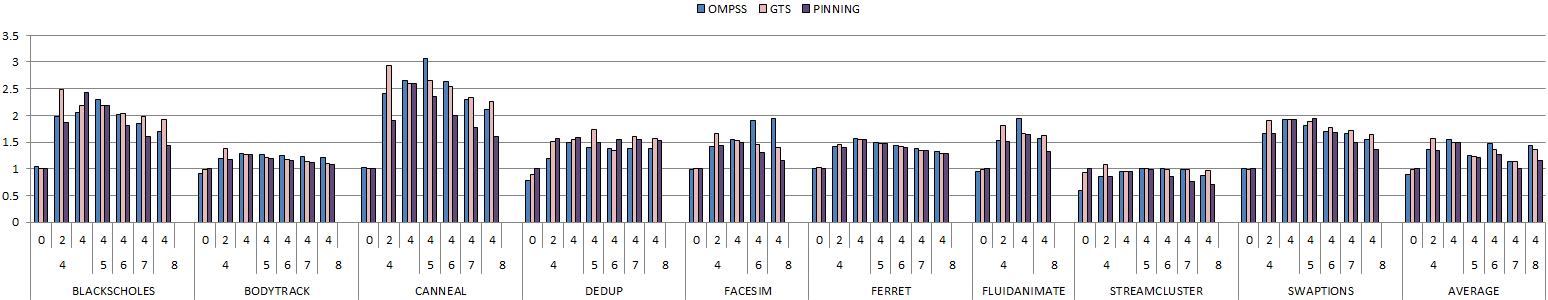
\includegraphics[width=1.0\textwidth]{figures/energy-parsec}%
% 	\vspace{-0.3cm}
% 	\caption{Energy consumption on a big.LITTLE processor with different $(F,N)$ configurations, where $F$ is the total number of big cores and $N$ the total number of cores. Results are normalized to running on four little cores with pinned Pthreads.}%
% 	\label{fig:all-energy}%
% \end{figure*}



We measure execution time, power, energy and EDP of nine 
applications from the PARSEC benchmark suite~\cite{Bienia:PhD2011}. We compare these metrics for 
three different scheduling approaches:
\begin{itemize}
\item \textit{Static threading}: scheduling decisions are made at the application level. The OS is not allowed to migrate threads between the clusters of big and little cores. 
\item \textit{GTS}\footnote{We choose to evaluate GTS instead of CS and IKS because it is the most advanced scheduling approach supported in the Linux kernel.}: dynamic coarse-grained OS scheduling 
using the GTS scheduler integrated in the Linux kernel~\cite{samsung, ARM} using the default 
PARSEC benchmarks. 
\item \textit{Task-based}: dynamic fine-grained scheduling at the runtime level with the task-based implementations of the benchmarks provided in PARSECSs~\cite{Chasapis:TACO2016}.
\end{itemize}


%%%%%%%%%%%%%%%%%%%%%%%%%%%%%%%%%%%%%%%%%%
%%%%%%%%%%%%%%%%%%%%%%%%%%%%%%%%%%%%%%%%%%
\subsection{Exploiting Parallelism in AMCs}
\label{sec:eval:A}

% \mm{This section should focus on identifying the problems that current applications have on an asymmetric/heterogeneous multicore. For example, static scheduling, homogeneous domain/workload partition. More dynamic applications, will scale better (bodytrack, dedup, ferret, freqmine, vips).}

This section examines the opportunities and challenges that current AMCs offer to emerging parallel applications. With this objective, we first evaluate a system with a constant number of four cores, changing the level of asymmetry to evaluate the characteristics of each configuration. In these experiments, all applications run with the original parallelization strategy that relies on the user to balance the application (\emph{Static threading}). We also evaluate the OS-based dynamic scheduling (\emph{GTS}) and the task-based runtime dynamic scheduling (\emph{Task-based}) for the same applications. 
% Figure~\ref{fig:ideal} shows the ideal speedup of the system for all the different combination of big and little cores. 
The system configurations evaluated in this section are:
i)~Four little cores (\texttt{0+4}); ii)~Two big and two little cores (\texttt{2+2}); and iii)~Four 
big cores (\texttt{4+0})

% \begin{itemize}
% \item Four little cores (\texttt{0+4})
% \item Two big and two little cores (\texttt{2+2})
% \item Four big cores (\texttt{4+0})
% \end{itemize}
For these configurations, Figure~\ref{fig:speedup4} shows the speedup of the PARSEC benchmarks with respect to running on a single little core. Figure~\ref{fig:power4} reports the average power dissipated on the evaluated platform. Finally, Figure~\ref{fig:energy4} shows the total energy consumed per application for the same configurations. Energy results are normalized to the energy measured with four little cores (higher values imply higher energy consumptions). Average EDP results are also included in this figure.

Focusing on the average performance results, we notice that all approaches perform similarly for the homogeneous configurations. 
Specifically, applications obtain the best performance on the configuration~\emph{4+0}, with an average speedup of 9.5$\times$ over one little core. 
When using four little cores, an average speedup of 3.8$\times$ is reached for all approaches. 
This shows that all the approaches are effective for this core count. 
In the configuration~\emph{2+2}, \emph{Static threading} slightly improves performance (5.0$\times$ speedup), while \emph{GTS} and \emph{Task-based} reach significantly higher speedups: 5.9$\times$ and 6.8$\times$, respectively.
\begin{figure*}[t]%
	\centering
	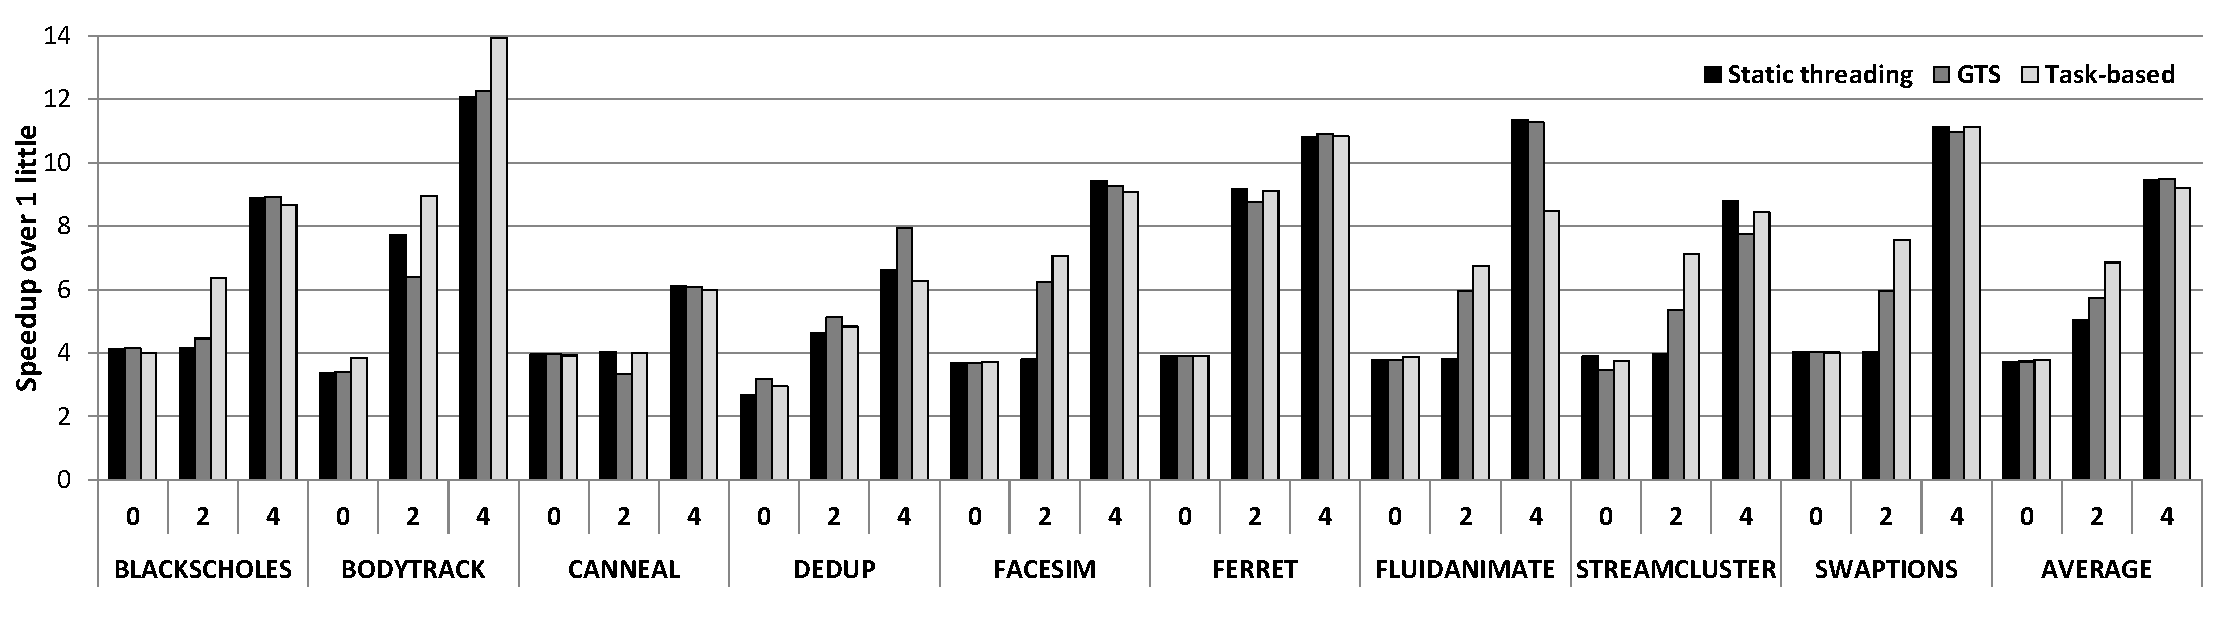
\includegraphics[width=1.0\textwidth]{figures/speedup-4_new.pdf}
	\vspace{-0.5cm}
	\caption{Execution time speedup over 1 little core for systems that consist of 4 cores in 
		total with 0, 2 and 4 big cores. Different schedulers at the application (\textit{static 
			threading}), OS  (\textit{GTS}) and runtime (\textit{task-based}) levels are considered.}
	%\caption{Performance improvements on a big.LITTLE processor with different $(F,N)$ configurations, where $F$ is the total number of big cores and $N$ the total number of cores. Results are normalized to running on four little cores with pinned Pthreads.}%
	\label{fig:speedup4}%
\end{figure*}
\begin{figure*}[t]%
	\centering
	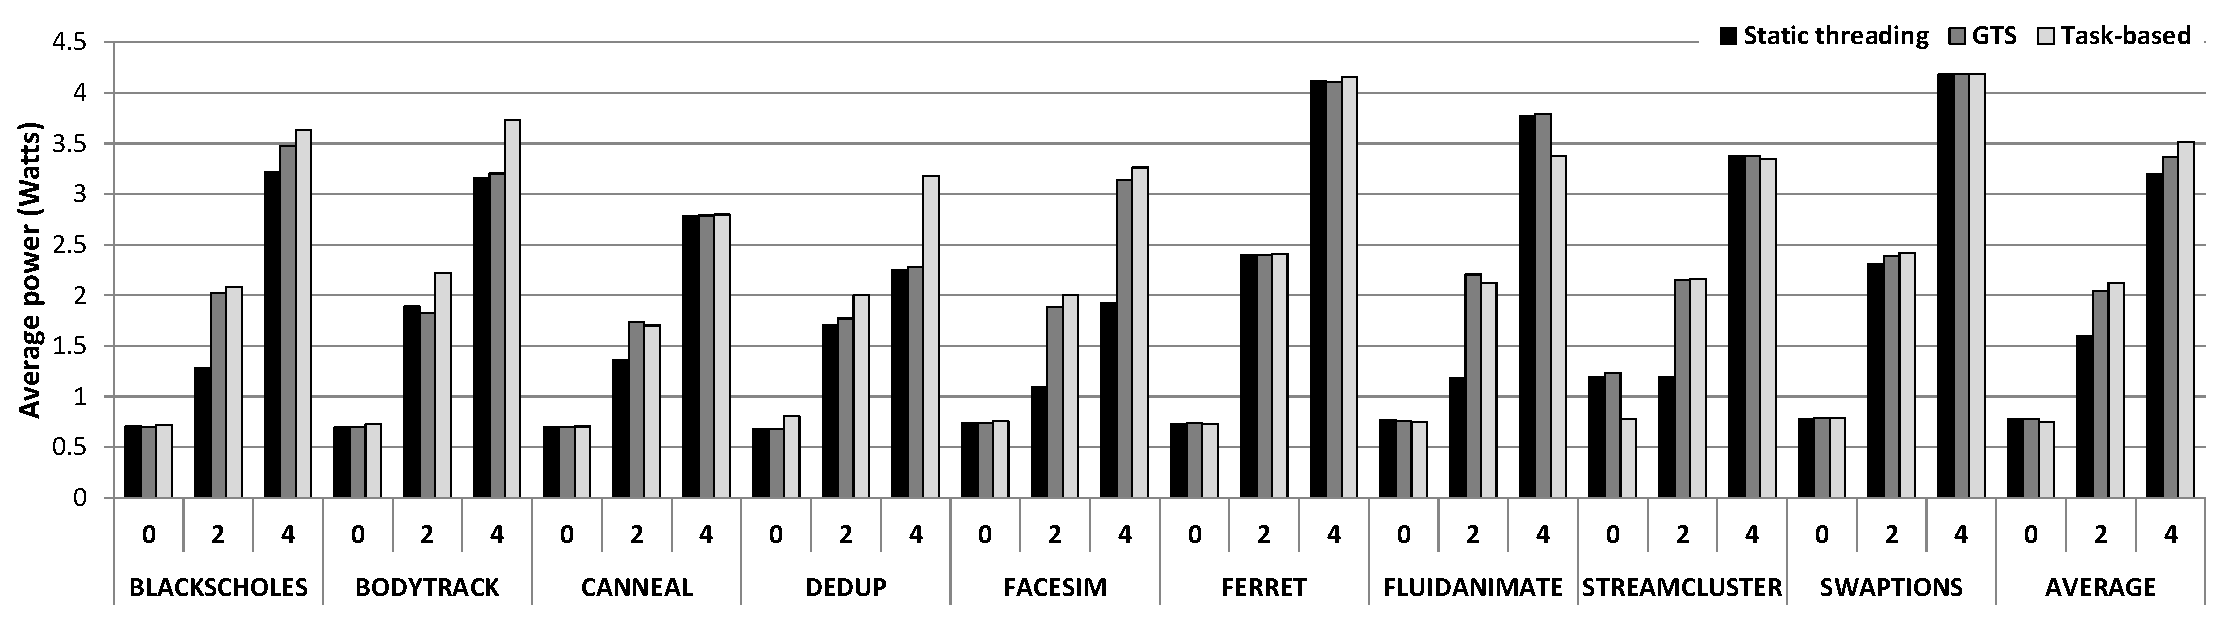
\includegraphics[width=1.0\textwidth]{figures/power4_new.pdf}
	\vspace{-0.5cm}
	\caption{Average power measurements on a 4-core system with 0, 2, and 4 big cores.}
	%\caption{Performance improvements on a big.LITTLE processor with different $(F,N)$ configurations, where $F$ is the total number of big cores and $N$ the total number of cores. Results are normalized to running on four little cores with pinned Pthreads.}%
	\label{fig:power4}%
\end{figure*}
\begin{figure*}[!h]%
	\centering
	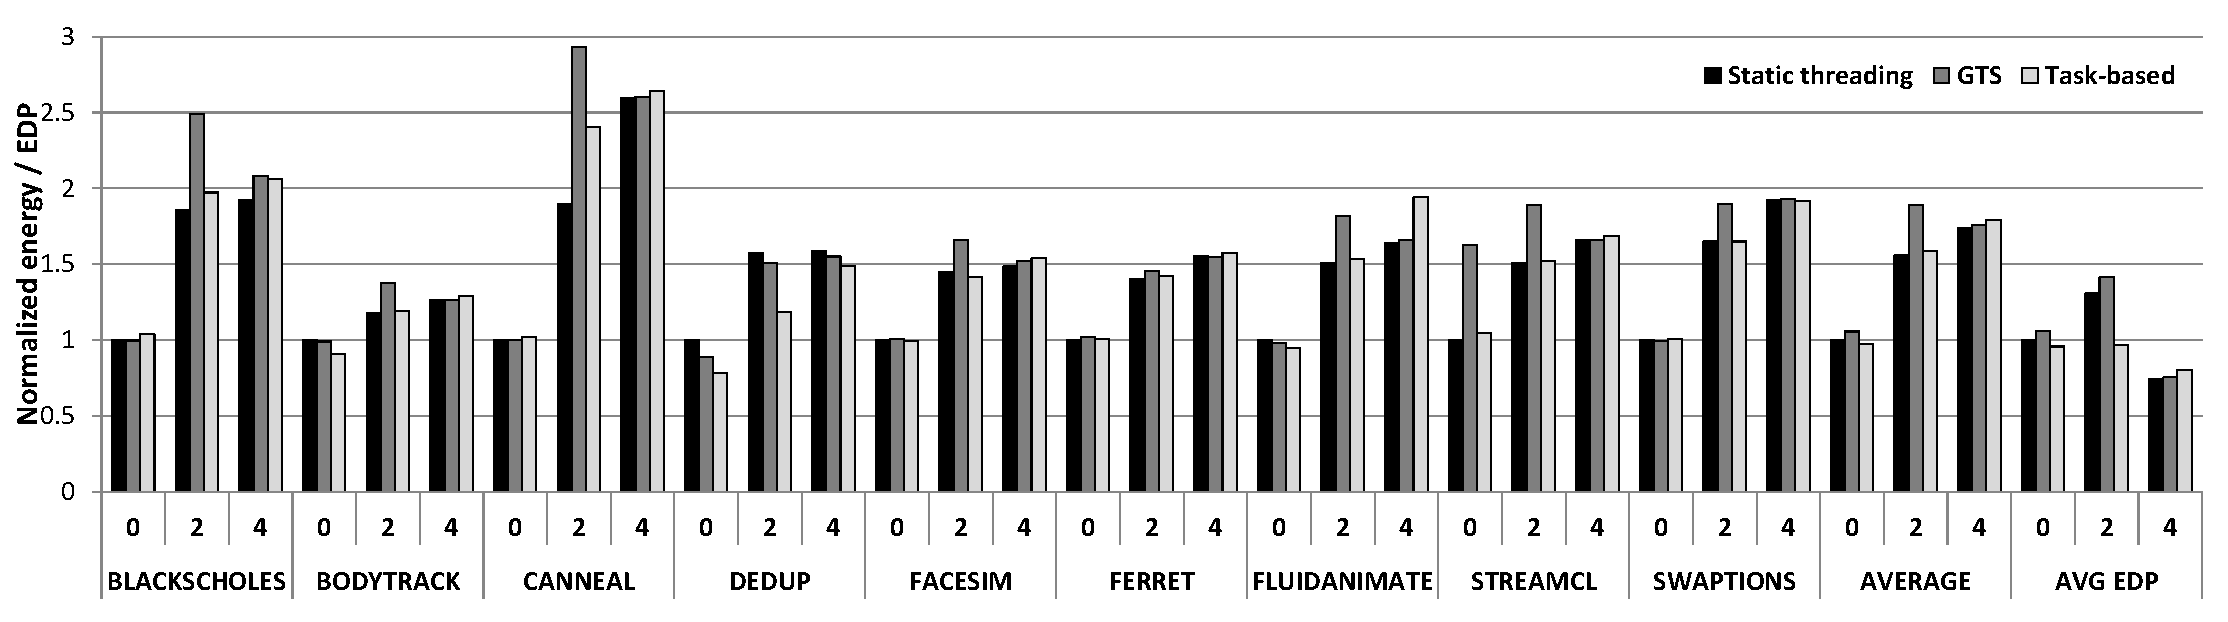
\includegraphics[width=1.0\textwidth]{figures/energy_EDP-4_new.pdf}
	\vspace{-0.5cm}
	\caption{Normalized energy consumption and average EDP on a 4-core system with 0, 2, and 4 big cores. Static threading on 4 little cores is the baseline in both cases. }
	%\caption{Performance improvements on a big.LITTLE processor with different $(F,N)$ configurations, where $F$ is the total number of big cores and $N$ the total number of cores. Results are normalized to running on four little cores with pinned Pthreads.}%
	\label{fig:energy4}%
\end{figure*}

Contrarily, in terms of power and energy, the most efficient configuration is running with four little cores, as the performance ratio between the different cores is inversely proportional to the power ratio~\cite{Greenhalgh2011}. On average, all the approaches reach a power dissipation of 0.75W for the \texttt{0+4} configuration, while \emph{Task-based} reaches 3.5W for the \texttt{4+0} configuration which is the one with the highest average power dissipation. In configuration \texttt{2+2}, average energy values for \emph{Static threading} and \emph{Task-based} are nearly the same, as the increase in power from 1.6W to 2.1W is compensated by a significant improvement in performance of 30\%.

Finally, in terms of EDP using the four big cores is the optimal, as the performance improvements compensate the increase in total energy. 
In configuration \texttt{2+2}, \emph{Task-based} achieves the same EDP results as in \texttt{0+4}, but with 81\% better performance. 
For the asymmetric configuration, \emph{Task-based} achieves the best performance-energy combination since its dynamic scheduling is effectively utilizing the little cores. 

%\texttt{0+4} reaches a power dissipation of 0.75W with all approaches, while \emph{Task-based} reaches 3.5W in configuration \texttt{4+0}.

%\kc{Consider removing this paragraph? It just mentions the obvious results that reviewers are complaining about...} Thus, if the number of cores remains constant, the best configuration in terms of performance and EDP corresponds to a symmetric configuration with big cores (e.g. \texttt{4+0}), while in terms of power and energy the best configuration corresponds to a symmetric configuration with little cores (e.g. \texttt{0+4}). 
% From the average energy-delay product (EDP) results in Figure~\ref{fig:energy4} we can approximate the configuration that achieves the highest performance with the best possible energy consumption. The configuration with the lowest EDP is the one with four big cores (\texttt{4+0}) since all the scheduling approaches manage to compensate the additional energy consumption with the speedup that can be achieved on this set-up. However, it is interesting to note that for the asymmetric configuration the \emph{Task-based} approach achieves the best combination of performance and energy since its dynamic scheduling approach is effectively utilizing the little cores. 

Next, we focus on the obtained results per benchmark. 
For applications with an extensive use of barriers (blackscholes, facesim, fluidanimate, streamcluster and swaptions) or with a memory intensive pattern (canneal), the extra computational power offered by the big cores in configuration \texttt{2+2} is not exploited. 
As a result with \emph{Static threading} performance is only slightly improved by 1\% on average when moving from \texttt{0+4} to the \texttt{2+2} configuration. 
This slight improvement comes at the cost of much more power and energy consumption (79\% and 77\% respectively).
These results are explained three-fold: i) load is distributed homogeneously among threads in some 
applications; ii) extensive usage of barriers force big cores to wait until little cores reach the 
barrier; and iii) high miss rates in the last-level cache cause frequent pipeline stalls and prevent 
to fully exploit the computational power of big cores. 
To alleviate these problems, the programmer should develop more advanced parallelization strategies that could benefit from AMCs, as performed in the remaining applications, or rely on dynamic scheduling at OS or runtime levels.

\textcolor{blue}{
\textbf{R1Q6:} GTS is a suitable alternative for barrier-synchronized applications (blackscholes, facesim, fluidanimate, streamcluster and swaptions) when asymmetry is introduced. 
GTS enhances performance as it is dynamically migrating the threads around the cores depending on the CPU utilization.
Thus it is expected that performance will increase compared to static threading for the asymmetric configuration. 
For these applications, the \emph{task-based} approach further improves GTS for the asymmetric configuration.
This is because \emph{task-based} schedules tasks among threads which is much more efficient than scheduling threads among cores.
}

The three remaining applications are parallelized using a pipeline model (bodytrack, dedup, and ferret)  with queues for the data-exchange between pipeline stages and application-specific dynamic load balancing mechanisms designed by the programmer.
As a result, \emph{Static threading} with these applications benefits from the extra computational power of the big cores in the configuration \texttt{2+2}. 
\textcolor{blue}{
\textbf{R1Q6:} Since \emph{Static threading} can already maintain load balance for these applications due to their implementation, there is no need for dynamic thread migration that is introduced by GTS.
}
%The advanced load balancing mechanisms introduced in these applications are not needed in the \emph{Task-based} code; 
\textcolor{blue}{
\textbf{R1Q4:} Using the \emph{task based} approach, the code of the application is simplified allowing the application to express even more parallelism as the runtime system automatically allows the overlapping of the different pipeline stages. 
This can be verified by the fact that bodytrack obtains higher performance with the \emph{task based} approach even for the symmetric configurations.
}
On the asymmetric configuration, \emph{Task-based} further improves the obtained performance, reaching a 13\% average improvement over \emph{GTS}. 
Clearly, these applications benefit in performance by the increased number of big cores, while power and energy are increasing since the big cores are effectively utilized.

%In these applications, all the approaches clearly outperform configuration \texttt{0+4}, while still increasing power and energy, as now all cores are busy (not only the little ones).

%the parallel regions to overlap more aggressively different stages of the pipeline. As a result, \emph{Task-based} further improves the obtained performance, reaching a 13\% average speedup over \emph{GTS}. In these applications, all the approaches clearly outperform configuration \texttt{0+4}, while still increasing power and energy, as now all cores are busy (not only the little ones).

Generally, relying on the programmer to statically schedule asymmetric configurations does not report good results, as it is very hard to predict the system's behavior at application-level. 
Only applications that implement advanced features with user-level schedulers and load balancing techniques, can benefit from asymmetry, at the cost of programmability effort.
Relying on the OS scheduler is a suitable alternative without code modifications, but relying on the runtime to dynamically schedule tasks on the asymmetric processor achieves much better performance, power and energy results.

%the developer did not consider it when designing the parallelization technique. When applications implement advanced features with user-level schedulers and load balancing techniques, applications can benefit from asymmetry, of course at the cost of programmability effort. A suitable alternative consists in relying on the OS system or the runtime to dynamically schedule tasks into the asymmetric processor, reaching much better performance, power and energy results in these systems.


%To estimate the best configuration when taking into account both performance and energy efficiency we have to 


%Relying on the programmer to benefit from asymmetry does not report good results, as the developer did not consider it when designing the parallelization technique. When applications implement advanced features with user-level schedulers and load balancing techniques, applications can benefit from asymmetry, of course at the cost of programmability effort. A suitable alternative consists in relying on the OS system or the runtime to dynamically schedule tasks into the asymmetric processor, reaching much better performance, power and energy results in these systems.

%, power or energy corresponds to a homogeneous configuration with in-order cores (power and energy) or big cores (performance). 

%In general relying on the programmer to benefit from asymmetry does not report good results, as the developer did not consider it when designing the parallelization technique. When applications implement advanced features with user-level schedulers and load balancing techniques, applications can benefit from asymmetry, of course at the cost of programmability effort. A suitable alternative consists in relying on the OS system or the runtime to dynamically schedule tasks into the asymmetric processor, reaching much better performance, power and energy results in these systems.
\iffalse
\mm{Figure~\ref{fig:energy4} also shows the average normalized results for EDP. In this case, lower is better. I didn't comment these results yet. With this metric, Task-based on 2+2 is as good as the others in 0+4 while we obtain better performance. This is interesting, but I'm not sure if it adds much with respect to the already presented numbers.}

\mm{I haven't commented much the results with the GTS scheduler. Maybe we should extend this part. Next, I put some sentences that might be useful, although I don't know where to put them.}

As described in Section~\ref{sec:scheduling}, the Global Task Scheduler (GTS) migrates tasks between cores in order to balance the load in the different cores of the heterogeneous processor. 

For fork-join + homogeneous load, the scheduler should be very effective, reaching the performance results of OmpSs. However, it is unaware of what it is moving around, which means that it might move a thread that is idle to a big core...

Consequently, for some benchmarks, the OS is making decisions without coordinating with the application scheduler and can worsen the performance. This should be the case of the applications with advanced load balancing techniques, but I still don't know if we will see this behavior.
\fi

% \begin{figure*}[t]%
% 	\centering
% 	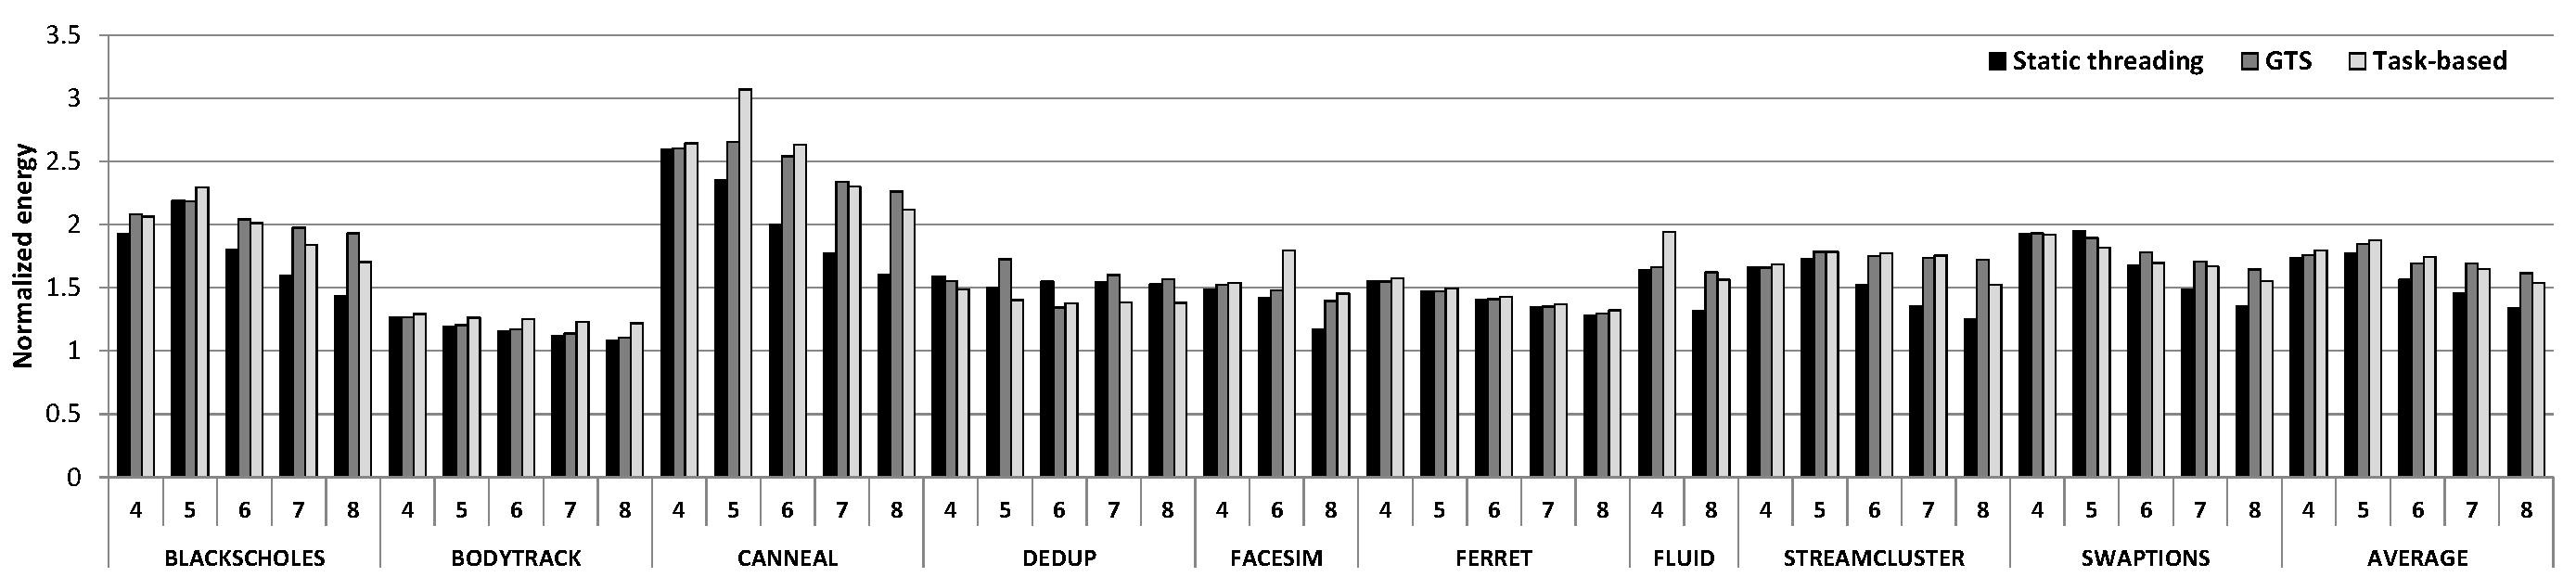
\includegraphics[width=1.0\textwidth]{figures/energy-4plus.pdf}
% 	\vspace{-0.5cm}
% 	\caption{Normalized energy consumption with respect to 4-little-static-threading energy consumption, when running on 4 to 8 cores and 4 of them are big}
% 	%\caption{Performance improvements on a big.LITTLE processor with different $(F,N)$ configurations, where $F$ is the total number of big cores and $N$ the total number of cores. Results are normalized to running on four little cores with pinned Pthreads.}%
% 	\label{fig:energy4plus}%
% 	\vspace{-0.3cm}
% \end{figure*}

% \begin{figure*}[t]%
% 	\centering
% 	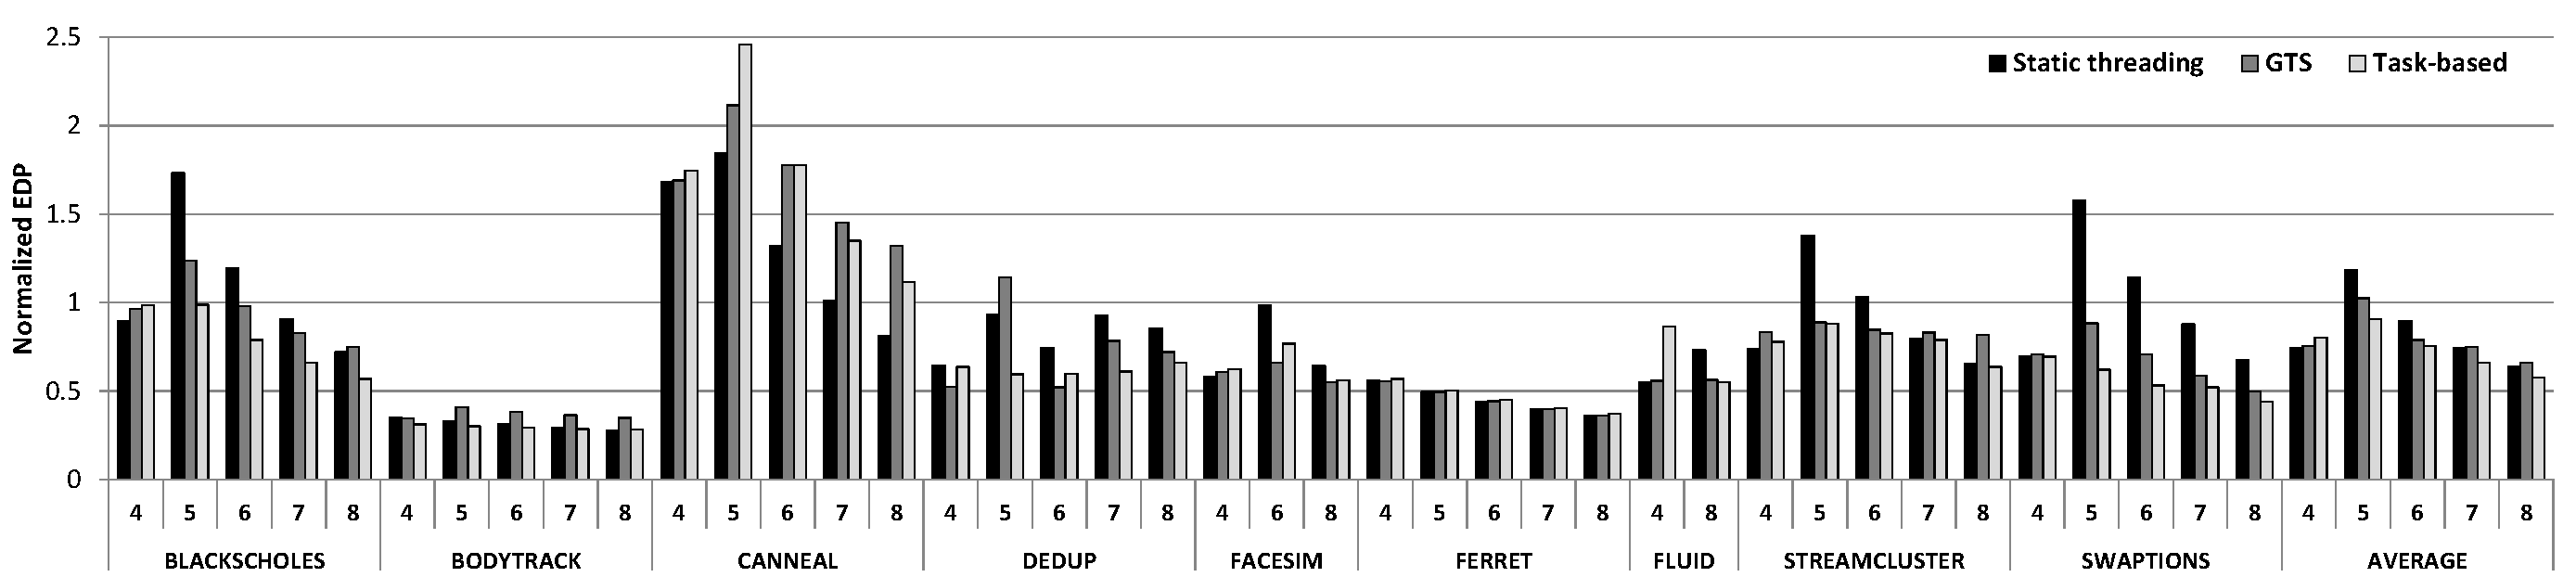
\includegraphics[width=1.0\textwidth]{figures/edp4plus.pdf}
% 	\vspace{-0.3cm}
% 	\caption{Normalized EDP when running on 5, 6, 7, or 8 cores and 4 of them are big}
% 	%\caption{Performance improvements on a big.LITTLE processor with different $(F,N)$ configurations, where $F$ is the total number of big cores and $N$ the total number of cores. Results are normalized to running on four little cores with pinned Pthreads.}%
% 	\label{fig:edp4plus}%
% \end{figure*}


%%%%%%%%%%%%%%%%%%%%%%%%%%%%%%%%%%%%%%%%%%
%%%%%%%%%%%%%%%%%%%%%%%%%%%%%%%%%%%%%%%%%%
\subsection{Adding Little Cores to an SMC}
\label{sec:eval:B}
In the following experiments, we explore if an application running on a symmetric multi-core (SMC) with big cores can benefit from adding small cores that help in its execution. Having more computational resources increases the ideal speedup a parallel application can reach, but it also introduces challenges at application, runtime and OS level. 
Thus, we examine how many small cores have to be added to the system to compensate the cons of having to deal with AMCs.

To evaluate this scenario, we explore configurations \texttt{4+0}, \texttt{4+1}, \texttt{4+2}, \texttt{4+3} and \texttt{4+4}. In these experiments, the number of big cores remains constant (four), while the number of little cores increases from 0 to 4. First we focus on the average results of speedup, power, energy and EDP, shown in Figure~\ref{fig:averages4plus}.

The speedup chart of Figure~\ref{fig:averages4plus} shows that \emph{Static threading} does not benefit from adding little cores to the system.
In fact, this approach brings an average 6\% slowdown when adding four little cores for execution (\texttt{4+4}).
This is a result of the static thread scheduling; because the same amount of work is assigned to each core, when the big cores finish the execution of their part, they become idle and under-utilized. 
GTS achieves a limited speedup of 8\% with the addition of four little cores to the \texttt{4+0} configuration. The addition of a single little core brings a 22\% slowdown (from \texttt{4+0} to \texttt{4+1}) and requires three additional little cores to reach the performance of the symmetric configuration (\texttt{4+3}).  Finally, the \emph{Task-based} approach always benefits from the extra computational power as the runtime automatically deals with load imbalance. Performance improvements keep growing with the additional little cores, reaching an average improvement of 15\% over the symmetric configuration when 4 extra cores are added. 
%An interesting observation is that according to the ideal speedup (Equation~\ref{eq.ideal} and Figure~\ref{fig:ideal}), the average ideal performance increase when moving from the \texttt{4+0} configuration to the \texttt{4+4} is 33\%, considering that the average performance ratio is 2.96$\times$ as shown in Table~\ref{tab:parsec}. Thus, the task-based approach achieves almost half of this theoretical ideal performance.

%the execution time speedup of the PARSEC benchmarks with respect to running in a single in-order core. 
%When looking at the average results, it is very interesting to see that the \emph{Static threading} approach clearly fails to benefit from the extra in-order cores. Even with four extra cores (configuration \texttt{4+4}), an average 15\% slowdown is obtained. \emph{GTS} also suffers a significant performance reduction when adding an extra little core (22\% slowdown) and requires three additional little cores to match the performance of the symmetric configuration. With an additional extra core, \emph{GTS} reaches an average 5\% speedup over the symmetric configuration. 


\begin{figure*}[t]%
	\centering
	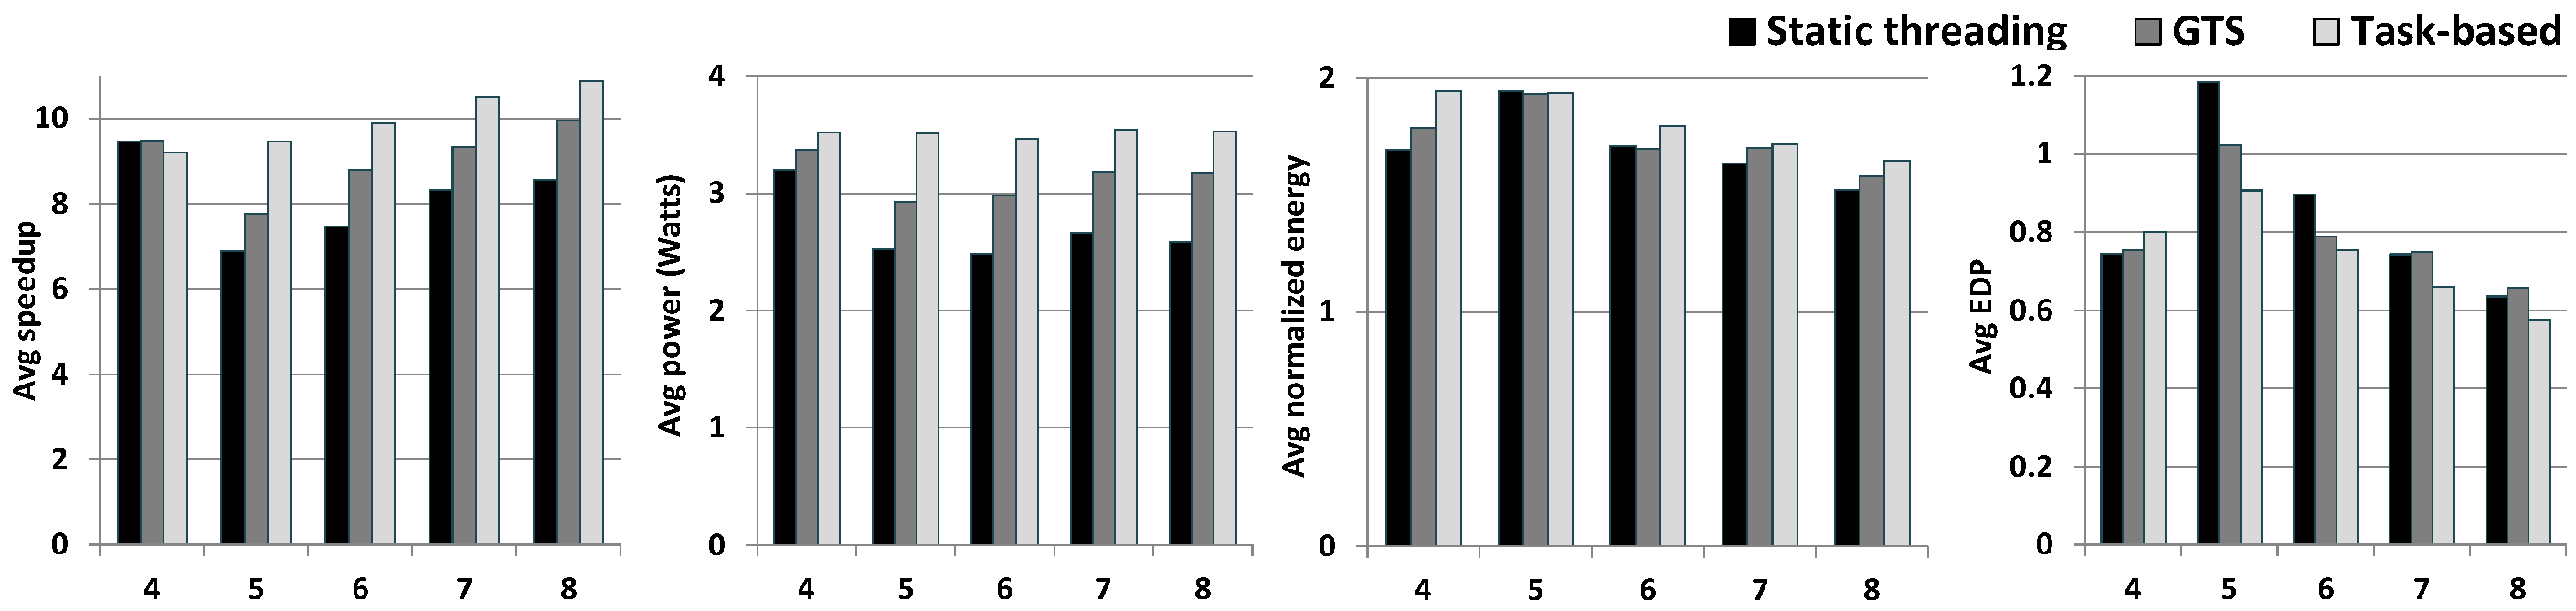
\includegraphics[width=\textwidth]{figures/averages_4plus_new.pdf}
	\vspace{-0.5cm}
	\caption{Average results when running on 4 to  8 cores with 4 of them big. Speedup is over 1 little core. Static threading on 4 little cores is the baseline of energy consumption and EDP}
	%\caption{Performance improvements on a big.LITTLE processor with different $(F,N)$ configurations, where $F$ is the total number of big cores and $N$ the total number of cores. Results are normalized to running on four little cores with pinned Pthreads.}%
	\label{fig:averages4plus}%
	\vspace{-0.3cm}
\end{figure*}

%In contrast, the \emph{Task-based} approach always benefits from the extra computational power as the runtime automatically deals with load imbalance. Performance improvements keep growing with the additional little cores, reaching an average improvement of 16\% over the symmetric configuration when 4 extra cores are added. Please, note that according to Table~\ref{tab:parsec} the performance ratio between big and little cores is 2.96$\times$, which means that the ideal speedup when adding 4 little cores to a system with 4 big cores is 1.33$\times$ ($\frac{2.96\cdot 4 + 4}{2.96\cdot 4}$). Thus, the \emph{Task-based} approach reaches half of the potential speedup on this asymmetric platform.

The power chart of Figure~\ref{fig:averages4plus} shows oppositional benefits among the three approaches. We can see that \emph{Static threading} and \emph{GTS} benefit from asymmetry, effectively reducing average power consumption.
\emph{Static threading} reduces power consumption when moving from the \texttt{4+0} to the \texttt{4+4} system by 23\% while \emph{GTS} does so by 6.2\%.
On the other hand, the \emph{task-based} approach keeps the big cores busy for most of the time so it maintains the average power nearly constant.


%In terms of power, the tradeoffs completely change. As shown in Figure~\ref{fig:power4plus}, \emph{Static threading} and \emph{GTS} always benefit from asymmetry, effectively reducing average power consumption. On average in configuration \texttt{4+4}, \emph{Static threading} and \emph{GTS} reduce power 23\% and 6.2\%, respectively, with respect to the symmetric multi-core. In contrast, the \emph{Task-based} approach always has all big cores busy and maintains overall power nearly constant. 

%In terms of energy, the third chart of Figure~\ref{fig:averages4plus} shows that the \emph{Static threading} significantly reduces energy consumption by 31\% when moving from \texttt{4+0} to the \texttt{4+4} configuration. As shown in the previous section, little cores are more energy efficient than big cores, at the cost of reduced performance. In the case of \emph{GTS} and \emph{Task-based}, at least two extra cores are needed to reduce energy. 
% In configuration \texttt{4+4}, energy is reduced by 31\% for \emph{Static threading}, 9.3\% for \emph{GTS}, and 16\% for \emph{Task-based}. Consequently, we can state that asymmetry reduces overall energy consumption, although the best configuration in terms of energy consists in using only four little cores.


The reduction in power, results to reduced average energy in the case of 
\emph{Static threading} in configuration \texttt{4+4}, as shown on the energy chart of 
Figure~\ref{fig:averages4plus}. As discussed in Section~\ref{sec:eval:A}, little cores are more energy 
efficient than big cores, at the cost of reduced performance. In all the approaches, at least two 
extra little cores are needed to reduce energy. In configuration \texttt{4+4}, energy is reduced by 
14\% for \emph{Static threading}, 15\% for \emph{GTS}, and 16\% for \emph{Task-based}. Consequently, we can state that asymmetry reduces overall energy consumption.
%, although the best configuration in terms of energy consists in using only four little cores (as average normalized energy is always above 1).

%--- ADD EDP results comments on average EDP
To see the impact on both performance and energy efficiency we plot the average EDP on the 
rightmost chart of Figure~\ref{fig:averages4plus}. In this chart the lower values are the better. The \emph{task-based} approach is the one that has the best performance-energy 
combination for the asymmetric configurations since it maintains the lowest EDP for all cases. 
\emph{Static threading} manages to reduce the average EDP by 6\% while \emph{GTS} and \emph{task 
based} approaches do so by 24\% and 36\% respectively.
%---
\begin{figure*}[t]%
	\centering
	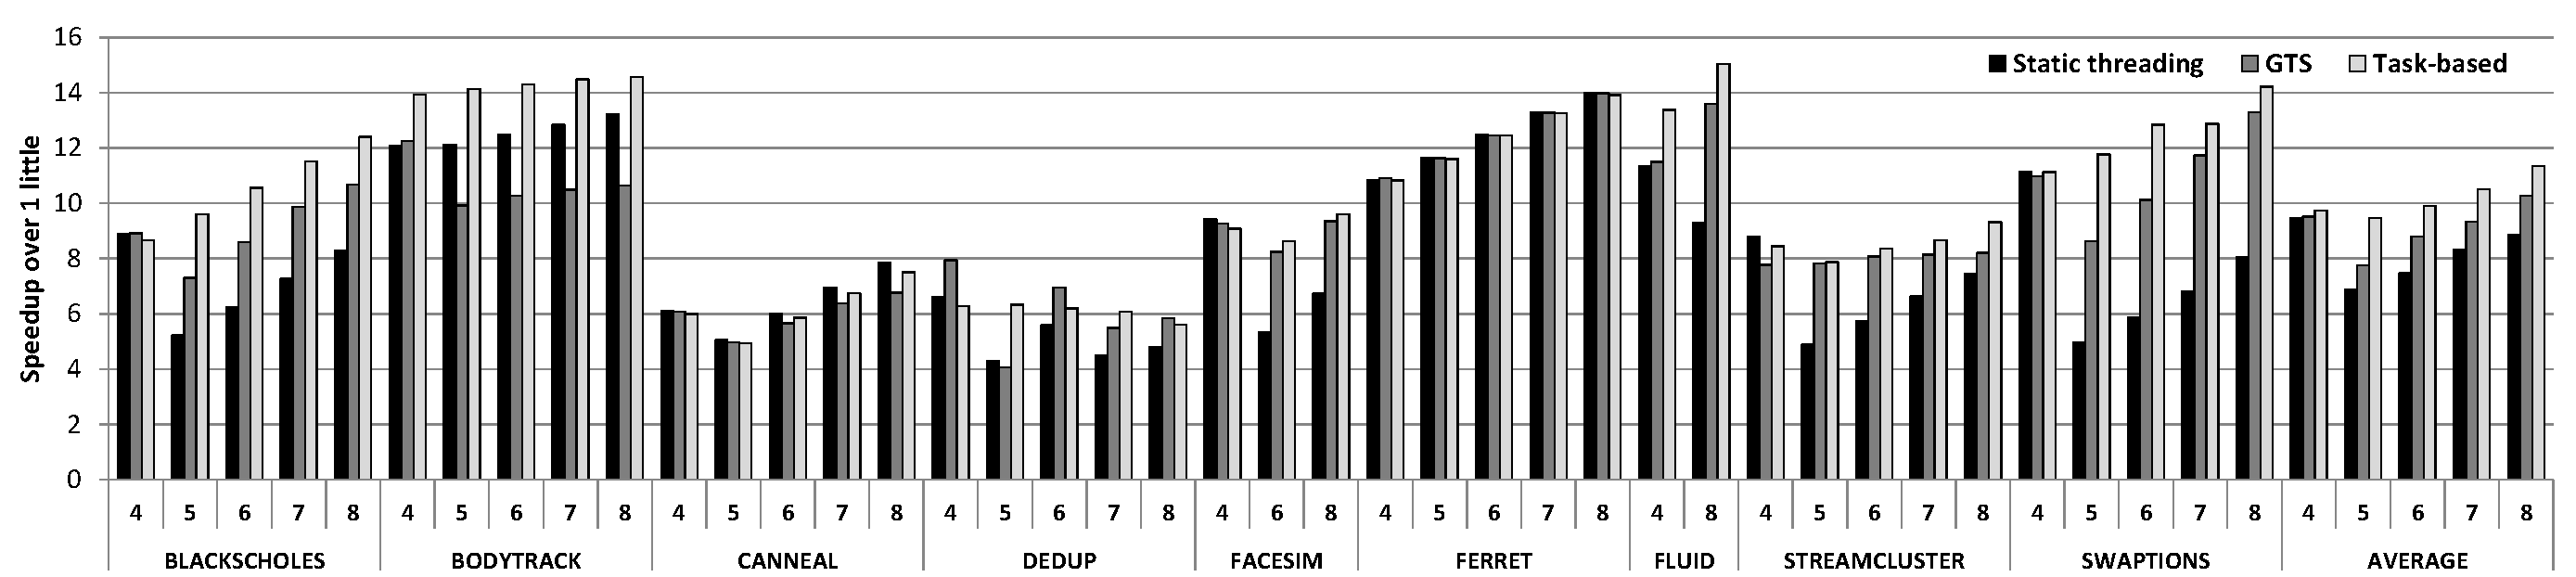
\includegraphics[width=1.0\textwidth]{figures/speedup-4plus.pdf}
	\vspace{-0.5cm}
	\caption{Speedup over 1 little core when running on 4 to 8 cores and 4 of them are big}
	%\caption{Performance improvements on a big.LITTLE processor with different $(F,N)$ configurations, where $F$ is the total number of big cores and $N$ the total number of cores. Results are normalized to running on four little cores with pinned Pthreads.}%
	\label{fig:speedup4plus}%
\end{figure*}
\begin{figure*}[t]%
	\centering
	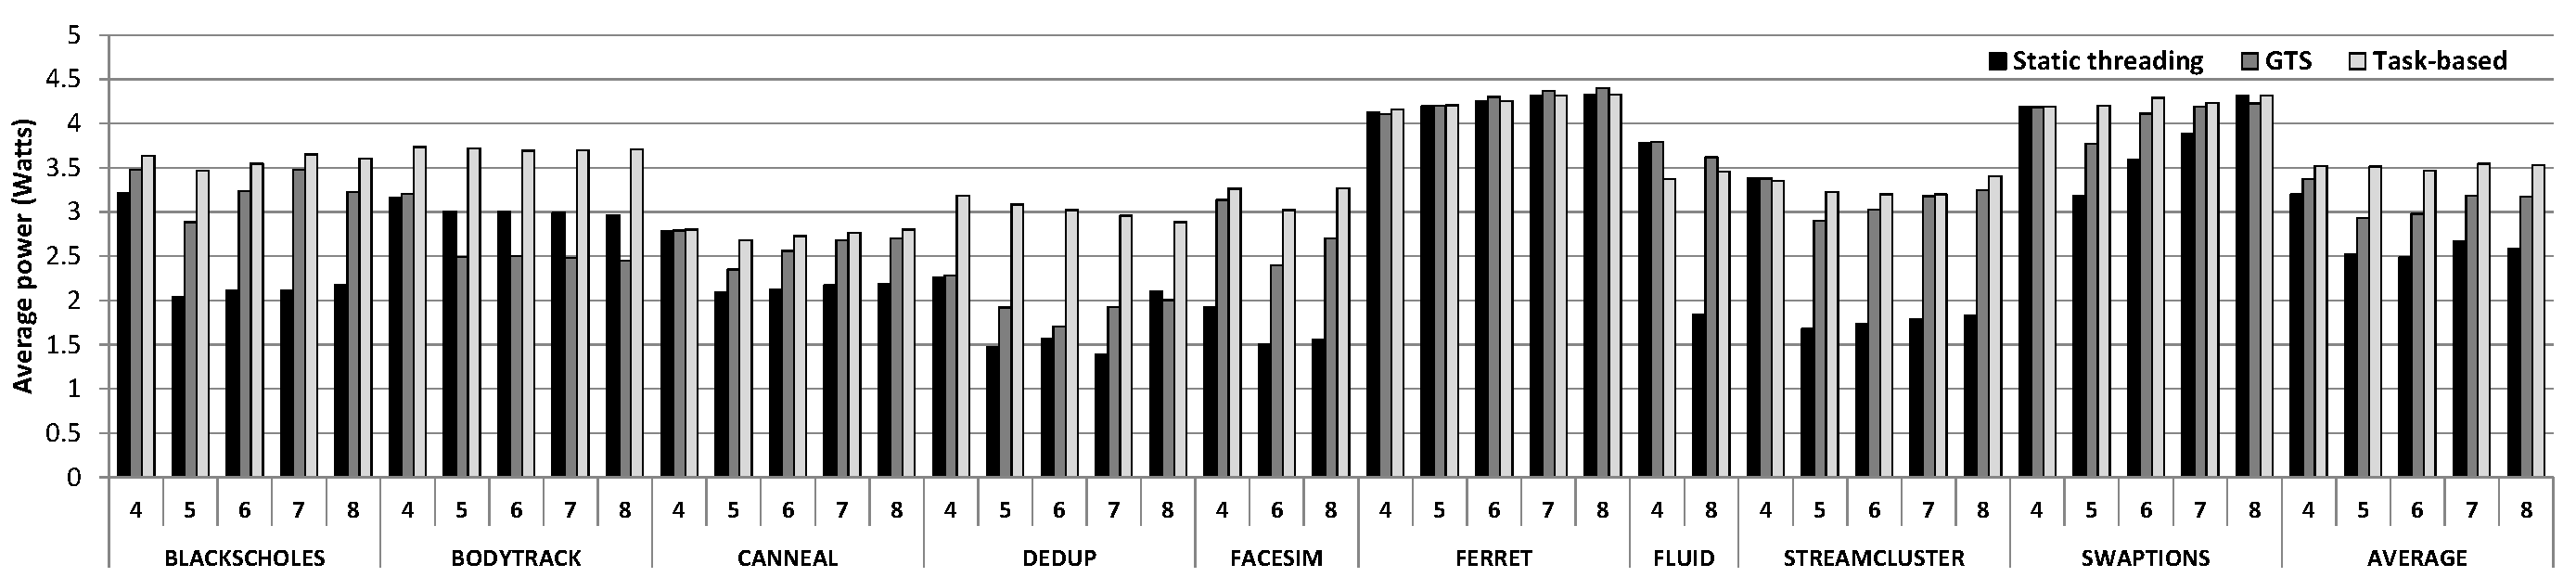
\includegraphics[width=1.0\textwidth]{figures/power4plus.pdf}
	\vspace{-0.5cm}
	\caption{Average power when running on 4 to 8 cores and 4 of them are big}
	%\caption{Performance improvements on a big.LITTLE processor with different $(F,N)$ configurations, where $F$ is the total number of big cores and $N$ the total number of cores. Results are normalized to running on four little cores with pinned Pthreads.}%
	\label{fig:power4plus}%
\end{figure*}

Figure~\ref{fig:speedup4plus} shows a more detailed exploration of the performance results. 
As Table~\ref{tab:parsec} shows, the applications with barrier synchronization are blackscholes, facesim, fluidanimate, streamcluster and swaptions. 
For these applications the most efficient system configuration with the \emph{Static threading} approach is the \texttt{4+0}. 
Little cores increase execution time due to load imbalance effects. 
\textcolor{blue}{
	\textbf{R1Q10:} \emph{GTS} and \emph{task-based} approaches overcome these issues by scheduling the load to the appropriate resources. 
	The differences in the improvement of the \emph{task based} and GTS solutions for these applications relies on the nature of each application and its parallel implementation.
	For example, swaptions, benefits more from the \emph{task based} and \emph{GTS} approaches than streacmluster.  
	This is because the task graph of streamcluster presents multiple small parallel regions that are spawned and synchronized. 
	Due to the multiple synchronization points, \emph{GTS} and \emph{task-based} cannot increase performance of streamcluster as much. 
	Contrarily, swaptions has less synchronization points, thing that allows GTS and task-based to exploit asymmetry during its longer parallel regions.
}
%we mention this later
%Since the big cores reach barriers earlier, power is reduced for these applications, as shown in Figure~\ref{fig:power4plus}. 
%Energy reduction is less significant with a few extra little cores as the performance degradation is higher, but as the number of little cores increases, energy is reduced. 



Applications with more advanced load balancing techniques like pipelined parallelism (bodytrack, dedup and ferret), benefit of the asymmetric hardware and balance the load among all the cores. 
\textcolor{blue}{As a result, the performance of \emph{Static threading} approach does not degrade when adding little cores as in the previous set of applications.
}
%As a result, performance improves as we increase the number of little cores. 
In the case of bodytrack, \emph{GTS} reduces performance by 15\% when 
adding four little cores. 
We attribute this to the cost of the thread migration from one core to the 
other in contrast to the \emph{Static threading} approach that does not add such overheads.
\textcolor{blue}{
\emph{Task based} approach also avoids these overheads and improves the performance of bodytrack by efficiently scheduling the tasks among threads.
}
%\kc{Please check this and let me know if makes sense. I had to write a comment for bodytrack.} 
In the case of dedup, results show more variability. This benchmark is very I/O intensive and, depending on the type of core that executes these I/O operations, performance drastically changes. In order to deal with this problem, a smarter dynamic scheduling mechanism would be required. 
%Ferret, obtains similar results with all approaches as its implementation is efficient with all scheduling approaches.
Finally, canneal does not scale according to its ideal speedup reported on Figure~\ref{fig:ideal} as it has a memory intensive pattern that limits performance.

Figure~\ref{fig:power4plus} shows the average power. The barrier-synchronized applications (blackscholes, facesim, fluidanimate, streamcluster and swaptions) reduce power because 
of their imbalance; since big cores have long idle times with the \emph{Static threading} approach, they do not dissipate the same power as \emph{GTS} and \emph{Task-based}.
%the big cores reach barriers earlier and remain idle, so power is reduced for the \emph{Static threading} approach compared to \emph{GTS} and \emph{Task-based}. 
For pipeline-parallel applications, both bodytrack and ferret maintain nearly the same 
power levels among the configurations for each scheduling approach. Dedup is an exception, as the 
results highly depend on the core that executes the aforementioned I/O operations. Yet, the 
effect of the lower power for \emph{Static threading} is observed in all the benchmarks and is because the big cores are under-utilized. %' long idle times.

%Each one of the pipeline-parallel applications (bodytrack, dedup, ferret) maintains nearly the same power levels among the configurations for each scheduling approach. 

%In these cases, the big cores do not remain as  Canneal also spends constant power among system configurations for the same reason.

%, while power consumption remains approximately the same. Consequently, total energy is reduced benefits in these asymmetric configurations.

%When focusing on the individual results per benchmark, the best configuration in terms of performance for applications with barriers (blackscholes, facesim, fluidanimate, streamcluster and swaptions) and with a memory intensive pattern (canneal) is \texttt{4+0}. Simple in-order cores increase execution time due to load imbalance effects. Since the big cores reach barriers earlier, power is reduced as a result for these applications, as shown in Figure~\ref{fig:power4plus}. Energy reduction is less significant with few extra little cores as the performance degradation is too high, but as the number of little cores increases, energy is reduced. 



%For applications with advanced load balancing techniques (bodytrack, dedup, and ferret), the application can take advantage of the asymmetric hardware and schedule load in all the cores. As a result, performance improves while we increase the number of little cores, while power consumption remains approximately the same. Consequently, total energy is reduced benefits in these asymmetric configurations. In the case of bodytrack, \emph{GTS} is having problems and a 20\% reduction in performance is obtained. \mm{Any idea why?}. In the case of dedup, results show more variability. This benchmark is very I/O intensive and, depending on which core executes these I/O operations, performance drastically changes. In oder to deal with this problem, a smarter dynamic scheduling mechanism would be required.
\textcolor{blue}{
\section*{Discussion}
\textbf{R1Q11: }Sections~\ref{sec:eval:A} and~\ref{sec:eval:B} explored the potential of different scheduling approaches when used on various workloads on an AMC. 
It was proven that current applications are not ready to utilize an AMC and that adding little cores to an SMC with big cores presents significant challenges for the application, OS and runtime developers. 
Little cores increase load imbalance and can degrade performance as a result. 
}

\textcolor{blue}{
A dynamic OS scheduler such as \emph{GTS} helps in mitigating load imbalance, providing an average performance increase of 10\%.
Barrier synchronized applications benefit more from the \emph{GTS} approach as the applications with more sophisticated scheduling techniques can utilize the little cores more efficiently even with \emph{Static threading}.
\emph{Task based} approach offers the optimal performance results for all types of workloads.
It improves \emph{Static threading} by 20\% on average by effectively balancing the load among big and little cores.
}

%Relying on the programmer to deal with this asymmetry is complex, but a dynamic OS scheduler such as \emph{GTS} helps in mitigating these problems, providing an average performance increase of 10\%. 
%However, the optimal performance results are obtained with the \emph{Task-based} approach, as they improve static threading by 23\% on average. 
In terms of power and energy, the AMC provides significant benefits, although the SMC with little cores remains the most energy-efficient configuration. 
\textcolor{blue}{
\textbf{R1Q9:} This is attributed to the differences of the designs of the big and little cores; little cores have been optimized for power efficiency while the design of the big cores targets higher performance levels at the cost of higher energy consumption.
}
The answer to the question of which system configuration provides the best power-performance balance, can be found on the average EDP chart of Figures~\ref{fig:energy4} and \ref{fig:averages4plus}, and is the use of the entire 8-core system with the \emph{Task based} approach.

%%%%%%%%%%%%%%%%%%%%%%%%%%%%%%%%%%%%%%%%%%
%%%%%%%%%%%%%%%%%%%%%%%%%%%%%%%%%%%%%%%%%%
\subsection{Programming Models for AMCs}

\begin{figure}
        \centering
        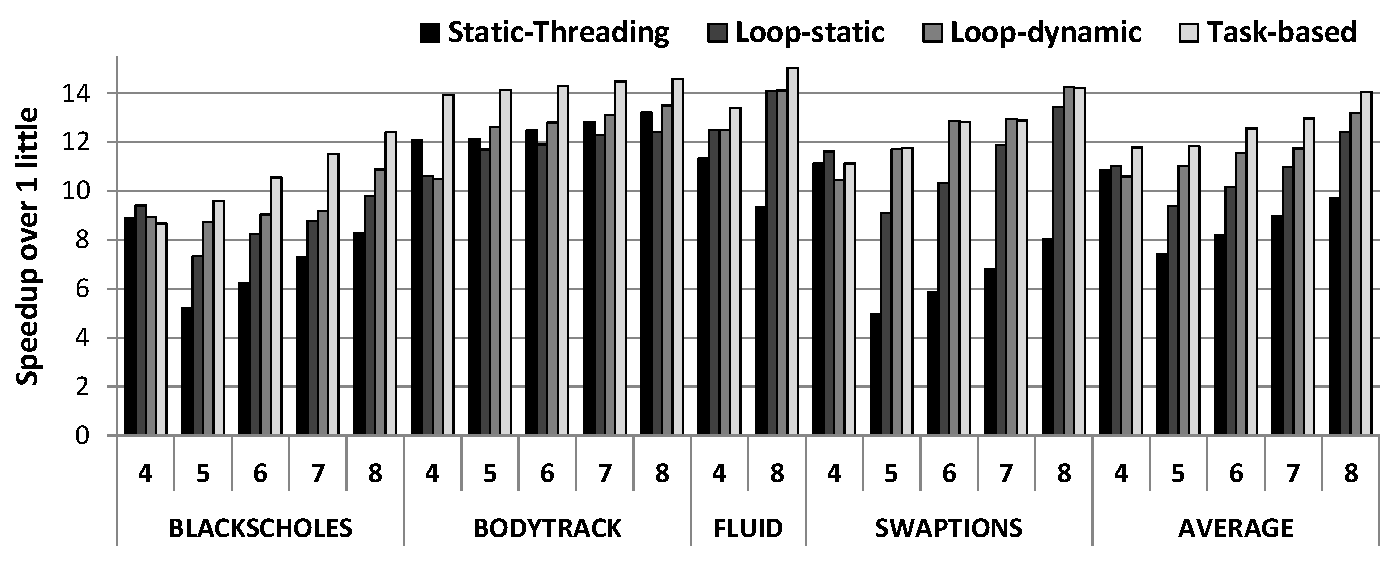
\includegraphics[width=\columnwidth]{figures/speedup-ompssVSopenmp_new}
        \vspace{-0.5cm}
        \caption{Speedup over 1 little core when running on 4 to 8 cores and 4 of them are big. 
Four different programming models are considered: Static threading using \texttt{pthreads}, 
parallel loops with static scheduling (loop static), parallel loops with dynamic scheduling (loop 
dynamic), and a task-based solution with dynamic scheduling (task-based).}%
        \label{fig:prog_models}%
\end{figure}

As we saw in the previous section, current implementations of parallel applications are not ready to fully take advantage of an AMC system.
Applications that are statically threaded using the low-level \texttt{pthreads} library usually suffer from load imbalance since their implementations assume that the work has to be equally distributed among the available cores. 
Implementing advanced load balancing schemes, such as
work pools, in \texttt{pthreads} requires a significant development effort.

As an alternative, many parallel applications are implemented using loop-based scheduling with the 
OpenMP \emph{parallel for} directives. 
In this case, the runtime library is in charge of scheduling work to the available threads in the system, either statically or dynamically, as described in Section~\ref{sec:runtime}.

We compare these solutions to the task-based approach evaluated in the previous sections. 
%Our goal is to evaluate the suitability of each programming model for asymmetric multi-cores. 
Figure~\ref{fig:prog_models} shows the results obtained from running blackscholes, bodytrack, fluidanimate and swaptions on all the scheduling models: static threading, static loop scheduling, dynamic loop scheduling and task-based scheduling. 
We chose these applications as they are the only ones implemented using the OpenMP loop directives.
%available in all the programming models under evaluation: \texttt{pthreads}, OpenMP loop directives and OpenMP tasks.

Looking at the average results in Figure~\ref{fig:prog_models}, we can observe that the task-based solution 
achieves the best results when the system is asymmetric. Task-based improves the static 
threading by up to 59\% on 5 cores, while dynamic loop scheduling improves by up to 54\%.
The OpenMP version with static scheduling reaches an average 26\% improvement over the static-threading approach with pthreads. 
\textcolor{blue}{
\textbf{R1Q12:} The main reason for this improvement is that the OpenMP programming model by default allows the OS scheduler to migrate threads to cores. 
Thus, in this case, GTS is allowed to move threads from little to big cores or vice versa, which differs to the static threading that pins the threads to the cores.
Similarly, loop-dynamic allows dynamic iteration scheduling as well as thread scheduling by GTS.
}

Taking a closer look to the results we observe that for bodytrack, an application with sophisticated parallelization techniques, static-threading achieves better results than loop-static.
This is because the static-threading implementation contains specific parallelization techniques that cannot be completely expressed using the loop-static method.
The loop-dynamic method improves performance for bodytrack by up to 4\% due to the runtime decisions of the iteration execution, but the optimal solution is offered by the task-based approach that achieves up to 16\% improvement over static-threading, due to the flexibility in expressing irregular parallelization strategies.
  
Blackscholes, fluidanimate and swaptions, consist of independent tasks and are a good fit for loop parallelism. 
The first observation is that all three applications benefit from the loop-static approach on an SMC with 4 big cores. 
Moreover, the task-based approach is still the optimal for blackscholes and fluidanimate, reaching up to 83\% improvement over static threading for 5 cores, while for swaptions both task-based and loop-dynamic are efficient, improving the baseline by up to 2.3$\times$.
%The difference in the characteristics of these applications relies on the task granularity; blackscholes consists of 6400 tasks that are about a hundred times smaller than each one of the 128 tasks of swaptions. 
%We attribute this to the fact that loop-dynamic is used in combination with GTS so this allows for an extra scheduling layer through the OS.
%This shows that loop-dynamic is more efficient on coarse-grained applications.
Finally, fluidanimate, that is also a fine-grained application that consists of 128\,500 tasks, also benefits from the task-based approach. 
For this benchmark, static and dynamic loop scheduling achieve similar performance; this is due to the limited parallelism per parallel region, as the loop-based implementation consists of multiple barriers between small parallel regions, fact that diminishes the effect of dynamic vs static scheduling. 
%Thus, if the loops have a small number of iterations, it makes no difference whether these iterations will be scheduled dynamically or statically as the resulting schedule will be the same.

% AR - this sounds wrong, no runtime activity in OMP static sched iteration distribution - This is because the static-scheduling overheads are inside the optimized OpenMP runtime system instead of the application's code. 


  \iffalse
However, 

The second solution is to transfer the responsibility to the runtime system so it dynamically 
schedules work to different core types based on work progress and core availability. The advantage 
is that the runtime system has knowledge of the application structure and parallel work boundaries 
so it can react with certain level of predictability. We evaluate dynamic scheduling on top of the 
existing work-sharing constructs in the applications with an OpenMP statically-scheduled 
implementation available. This requires code transformation that are straightforward in many cases.

We finally evaluate the impact of using a inherently load-balanced execution model such that of 
task-based programming models. Recent examples~\cite{Ayguade:TPDS2009, OpenMP4.0:Manual2013, 
OmpSs_PPL11, Zuckerman:EXADAPT2011, Bauer.2012.SC, Vandierendonck:PACT2011, Vandierendonck:Hyperq} 
include clauses to specify inter-task dependences and remove most barriers which are the major 
source of load imbalance on AMCs.

Comment new figure: Figure~\ref{fig:prog_models}.
Figure~\ref{fig:prog_models} shows the speedup over one little core of blackscholes, bodytrack and swaptions for task-based and static threading solutions compared to loop scheduling solutions. 
The applications are implemented using the OpenMP 2.0 directives for loop scheduling. 
We compare both dynamic and static loop scheduling and the results show that the task-based approach on average outperforms this programming model.
Bodytrack, that consists of highly sophisticated parallel programming techniques performs better with the task-based model as the freedom of task creation and the specification of dependencies helps on a more efficient implementation. 
On the other hand we can observe different behaviour between the highly parallel benchmarks blackscholes and swaptions.
These two benchmarks consist of independent tasks but they show oppositional benefits in terms of the optimal programming model.
Swaptions consists of 128 tasks each of them taking 100$\times$ more time than the blackscholes tasks. 
Blackscholes on the other hand consists of 6400 tasks. 
So, blacksholes is a more fine grained benchmark that lets the task-based programming model to overcome the overheads and increase performance in return.
The loop scheduling work better when the number of tasks is limited and the parallelization is regular.
\fi

%%%%%%%%%%%%%%%%%%%%%%%%%%%%%%%%%%%%%%%%%%
%%%%%%%%%%%%%%%%%%%%%%%%%%%%%%%%%%%%%%%%%%
\if 0 
\subsection{Power Consumption Analysis over Time}

%To understand in detail some of the behaviours pointed out in the last sections, we provide detailed power measurements during the whole execution of the streamcluster benchmark. 

This section provides a detailed analysis of the power consumption over time for one of the evaluated applications, streamcluster.
We choose this application as an illustrative example of the utilization of the processor resources 
(performance and power) with the different evaluated approaches.
Figure~\ref{fig:streamcluster_consumption_evolution} shows the power samples measured over the 
execution time of streamcluster when running on 8 cores (\texttt{4+4} configuration).
On the left part of the figure we plot the power samples of only the 4 big cores, while on the right part we plot the total power samples of all the big and the little cores.
Both charts contain this information for the three scheduling approaches evaluated in this paper (\emph{Static threading}, \emph{GTS} and \emph{Task-based}).
As expected, all the approaches display the same five execution phases throughout the execution, as this benchmark is processing five large chunks of points.
Seemingly the power samples of the big-core cluster slightly outreach 3W for the \emph{GTS} and \emph{Task-based} approaches, while for \emph{Static threading} they remain close to 1.5W. As shown in Figure~\ref{fig:power4}, steamcluster dissipates 1.2W when running on 4 little cores.
Thus, this proves that the \emph{GTS} and \emph{Task-based} approaches better utilize the big cores and, in contrast, the big cores remain idle for a significant amount of time with the \emph{Static threading} strategy.

On the right of Figure~\ref{fig:streamcluster_consumption_evolution}, where the power samples of the whole chip are plotted, the \emph{Task-based} approach has power samples slightly higher than the \emph{GTS} approach:
with the \emph{Task-based} approach, measured power is around 4.0W, while with \emph{GTS} observed power is around 3.6W.
The main difference between these measurements and the ones on the left chart of the same figure is the power consumption of the little cores. 
Thus we derive that both \emph{GTS} and \emph{Task-based} fully utilize the big cores in the system, but the \emph{Task-based} approach utilizes the little cores better than \emph{GTS}. In contrast, \emph{Static threading} does not take advantage of the computational power of this AMC for the streamcluster benchmark.

Despite the fact that performance and power consumption of the little cores are much smaller than the ones of the big cores, the \emph{Task-based} approach significantly reduces the execution time of streamcluster from 374 seconds to 312 seconds. A more effective usage of the little cores at the cost of slightly higher power consumption leads to these results. This clearly demonstrates the benefits of runtime system-based programming models against thread-based approaches in AMC systems.
\fi
%fully using the little cores is extremely important since the task-based approach reduces execution time from 374 to 312 
%without spending much more power by fully exploiting the little cores.


%Figure~\ref{fig:streamcluster_consumption_evolution} contains the measured power consumption per time when streamcluster runs on the 8 cores of the octodroid platform.
%On the left of figure~\ref{fig:streamcluster_consumption_evolution}, we can see the power consumption of just the big cores and on the right the consumption of the whole chip.
%\mc{We need to understand and explain the power dissipation of what hw components (private caches, cores, ...) is being measured.}
%Measurements are shown for the three parallel strategies considered in this paper: \emph{Static Threading}, \emph{GTS} and \emph{task-based}.
%Interestingly, the three considered strategies display the same 5 execution phases, which is obviously expected.
%In terms of power consumption of just the big cores, we can see how these cores dissipate slightly more than 3 Watts when run streamcluster either with the \emph{GTS} or the \emph{Task-based} approaches.
%The \emph{Static threading} approach makes the big cores to dissipate much less power, around 1.5 Watts. 


%This means that the GTS and the task-based approaches use extensively the big cores and, in contrast, the big cores spend a significant amount of idle time under the static threading regime.

%Right of Figure~\ref{fig:streamcluster_consumption_evolution} shows the power consumption when the whole chip is measured.
%In this scenario, things slightly change since the task-based approach spends more power (around 4 Watts most of the time) than the GTS technique (around 3.6 Watts).

%Since the only difference between these measurements and the ones on top of Figure~\ref{fig:streamcluster_consumption_evolution} is the power consumption of the little cores, we can derive that
%the task-based approach uses the little cores much more intensely than the GTS policy, since these cores dissipate much more
%power under the task-based regime than the GTS one. 


%Despite the fact that performance and power consumption of the little cores are much smaller than the ones of the big cores, fully using the little cores is extremely important since the task-based approach reduces execution time from 374 to 312 without spending much more power by fully exploiting the little cores. 

%These results clearly demonstrate the benefits of task-based programming models against thread-based approaches in asymmetric multi-core systems.



%%%%%%%%%%%%%%%%%%%%
%%%%%%%%%%%%%%%%%%%%
\section{Related Work}
\label{sec:related}
\iffalse
\mm{I don't think we have to focus so much in schedulers. I would also add other things, like HW support, runtime extensions, or application modifications for heterogeneous systems.}

\mm{Missing refs: the CATS ICS 2015~\cite{Chronaki:ICS2015}, all OmpSs support for GPU+CPU systems and other heterogeneous platforms~\cite{Bueno:IPDPS2012,Planas:IPDPS2013,Planas:ICCS2015}.} 

\mm{Also missing all the papers from Onur Mutlu on Asymmetric Multicores}

\mm{Maybe we can include some performance characterization of real machines. At BSC, we have a good paper track on this: POWER5 decode priorities (ISCA 2005), POWER7 prefetcher (PACT), UltraSPARC T1 (MICRO, Petar), etc.}
%%%%%%%%%%%%%%%%%%%%%%%%%%%%%%%%%%%%%%%%%%%%%%%%%%
\fi


%\mm{The past work has predominantly considered sequential applications and has mostly been simulation-based, which limits the size of possible workloads and the ability to accurately measure performance and energy. We found that our conclusions differ as a result of these differences in experimental methods.}

There has been a lot of studies on asymmetric multi-core systems. Some works focus on the design of the system, while other works explore the challenges that appear in efficiently utilizing such a heterogeneous system.
Kumar et al~\cite{Kumar_micro_2003} present the idea of an asymmetric multi-core system and proposed a feedback-based way to dynamically migrate processes among the different cores. 
%Their approach led to energy savings but at the cost of performance degradation. 
To determine the core that most effectively executed a workload, Kumar et al~\cite{Kumar:ISCA2004} proposed the use of sampling. The proposed method minimizes the execution time of each single thread and increases performance. Other studies focused on the pipeline design of such asymmetric systems and the area that should be devoted to each component in the system~\cite{Balakrishnan:ISCA2005, Morad_area_based}. Other works on asymmetric systems focus on hardware support for critical section detection~\cite{Suleman:APLOS2009} or bottleneck detection~\cite{Joao:ASPLOS2012,Joao:ISCA2013}.
%Other authors proposed hardware support to detect critical sections of a parallel application and schedule the most critical ones on the big cores~\cite{Suleman:APLOS2009, Joao:ASPLOS2012,Joao:ISCA2013}. 
These approaches are orthogonal to the approaches evaluated in this paper and could benefit from them to further improve the final performance of the system.

Process scheduling on asymmetric systems is one of the most challenging topics in this area of study.
Bias scheduling~\cite{Koufaty_bias} is an OS scheduler that characterizes the running 
threads according to their memory or execution intensity. 
It then schedules the computation intensive threads to the big cores of the system while the memory intensive threads to the little cores of the system.
The experimental evaluation is done on Intel Xeon processors and the heterogeneous system is emulated by changing the configuration of three out of the four cores of the processor.
Cong et al propose the Energy-Efficient~\cite{Cong_quickIA} OS scheduler based on energy estimation. The evaluation is performed on the Intel QuickIA~\cite{quickIA} platform that integrates an Intel Xeon with an Atom processor. 
%Code instrumentation is used to schedule different phases of the application on each processor. However, the separate core and memory subsystems in these architectures incur power and performance overheads for application migration, which makes dynamic mapping ineffective for fine-grained migration
Van Craeynest et al.~\cite{VanCraeynest_fairness} propose the fairness-aware OS scheduler that 
focuses on asymmetric multi-core 
architectures. 
%They focus on heterogeneous single-ISA architectures and they use some of the applications evaluated in our paper but their research lacks the real heterogeneous system; instead they simulate a heterogeneous processor with big and little cores to estimate performance and fairness (not energy).
The performance impact estimation (PIE) scheduler~\cite{VanCraeynest_PIE} is based on the impact of MLP and ILP on the overall CPI and focuses on improving performance.
The scheduler predicts the impact of each different core-type of the system on the MLP, ILP and it assumes hardware support for CPI. 
%The evaluation of this paper is performed through simulation by mimicking a heterogeneous system like ARM big.LITTLE. Further there are no energy or power measurements.
Rodrigues et al~\cite{Rodrigues_thread_scheduling} propose a thread scheduling technique that estimates power and performance when deciding to assign a thread to a specific core of the heterogeneous system. 
%However their evaluation is based on simulated results and not on a real platform. They have info for power.
Finally, Energy-Aware Scheduling (EAS) is an on-going effort in the Linux community to introduce 
the energy factor in the OS scheduler~\cite{EAS, EAS_Linux}. It is based on performance and power 
profiling to set performance and power capacities and let the Linux completely fair scheduler 
assign slots to processes considering the different core capacities. EAS is not yet part 
of the Linux kernel and, therefore, GTS is the most sophisticated state of the art scheduling method 
in production on current big.LITTLE processors.





%Van Craeynest et al. [33] proposed the PIE model for heterogeneous multi-core with big out-of-order and small in-order cores. The PIE model uses simple analytical models to predict how core architecture affects exploitable ILP and MLP and its impact on CPI. Scheduling using the PIE model assumes hardware support for computing CPI stacks as well as a few model inputs. The hardware cost is limited to roughly 15 bytes of storage. Again, all of this prior work focused on optimizing system throughput while running multi-program workloads, and none looked into optimizing fairness nor multithreaded application scheduling.

%Moreover, there have been many works for the efficient task scheduling on heterogeneous systems.
%In the literature there exist numerous dynamic or static scheduling algorithms for heterogeneous multi-cores with comprehensive experimental evaluation.

Similar to OS scheduling approaches there have been many task scheduling approaches that are directed for utilizing asymmetric systems.
The Levelized Min Time~\cite{Hetero95} heuristic first clusters the tasks that can execute in parallel (\textit{levels}) and then it assigns priorities to them, according to their execution time.
The Dynamic Level Scheduling algorithm~\cite{Hetero93} assigns the tasks to the processors according to their \textit{dynamic level} (DL).
% which is \textit{DL(n) = SL(n) - earliest exec time(n)}. 
%Random graph generators on simulated heterogeneous processors. 
Heterogeneous Economical Duplication (HED)~\cite{Dup09} duplicates the tasks in order to be executed on more than one cores but it then
%performs task duplication in an economical manner as it 
removes the redundant duplicates if they do not affect the makespan. 
CATS scheduler~\cite{Chronaki:ICS2015} is designed for asymmetric systems like big.LITTLE and dynamically schedules the \textit{critical} tasks to the big cores of the system to increase performance. 
Topcuoglu et al proposed the Heterogeneous Earliest Finish Time (HEFT) scheduler that statically assigns each task to the processor that will finish it at the earliest possible time. To do so, it keeps records with the task costs for each processor type.
%The Heterogeneous Earliest Finish Time (HEFT) algorithm \cite{HEFT} maintains a list of tasks sorted in decreasing order of their \textit{upward rank}. At each schedule step, HEFT assigns the task with the highest \textit{upward rank} to the processor that finishes the execution of the task at the earliest possible time. Lack of desktop applications and no mention of real heterogeneous system.
They also proposed the Critical Path on a Processor (CPOP) algorithm \cite{HEFT} that maintains a list of tasks and statically identifies and schedules the tasks belonging to the critical path  to the processor that minimizes the sum of their execution times. 
%Critical Path on a Processor (CPOP) algorithm \cite{HEFT} also maintains a list of tasks but, in this case, tasks are sorted decreasingly according to their \textit{upward rank + downward rank}. 
%The tasks with the highest \textit{upward rank + downward rank} are the tasks that belong to the critical path and these are sent to the \textit{critical path processor} that is the one that minimizes the sum of their execution times. Lack of desktop applications and no mention of real heterogeneous system.
The Longest Dynamic Critical Path (LDCP) algorithm \cite{LDCP} identifies the tasks that belong to the critical path and schedules them with higher priority.

%computes the critical path at each schedule step by scheduling the tasks with the highest \textit{URank} (upward rank) first. 
%Every time a task is scheduled, the \textit{computation cost matrix} is updated with the new timing values for the task. 

%More related work can be found in \cite{CrParTree, CrPathDup}

All these works reflect the remarkable research that is taking place on asymmetric systems. 
However we consider that their experimental evaluation is limited for three main reasons:
i)~Their experimental evaluation is done through a simulator or emulation of an asymmetric 
system \cite{Kumar_micro_2003, Kumar:ISCA2004, Morad_area_based, Balakrishnan:ISCA2005, 
Koufaty_bias, VanCraeynest_fairness, VanCraeynest_PIE, Rodrigues_thread_scheduling, Hetero93, 
Hetero95, Dup09, Suleman:APLOS2009, Joao:ASPLOS2012,Joao:ISCA2013};
ii)~The evaluated applications are either random task dependency graph generators or scientific 
kernels and micro-benchmarks \cite{Hetero93, Chronaki:ICS2015, HEFT, LDCP}.
iii)~Their evaluation does not focus on power and energy consumption \cite{Kumar:ISCA2004, 
VanCraeynest_fairness, VanCraeynest_PIE, Hetero93, Hetero95, Chronaki:ICS2015}.

% \begin{itemize}
%   \item Their experimental evaluation is done through a simulator or emulation of an asymmetric system \cite{Kumar_micro_2003, Kumar:ISCA2004, Morad_area_based, Balakrishnan:ISCA2005, Koufaty_bias, VanCraeynest_fairness, VanCraeynest_PIE, Rodrigues_thread_scheduling, Hetero93, Hetero95, Dup09, Suleman:APLOS2009, Joao:ASPLOS2012,Joao:ISCA2013}.
%   \item The evaluated applications are either random task dependency graph generators or scientific kernels and micro-benchmarks \cite{Hetero93, Chronaki:ICS2015, HEFT, LDCP}.
%   \item Their evaluation does not focus on power and energy consumption \cite{Kumar:ISCA2004, VanCraeynest_fairness, VanCraeynest_PIE, Hetero93, Hetero95, Chronaki:ICS2015}.
% \end{itemize}
This paper presents a comprehensive evaluation of performance, power and energy on a real asymmetric system of parallel desktop applications.
Another important point that this paper makes is the impact of using different big and little core counts which is not present in previous works \cite{Cong_quickIA}.









































\iffalse
%%%%%%%%%%%%%%%%%%%%%%%%%%%%%%%%%%%%%%%%%%%%%%%%%%
This is an evaluation paper of isca 2015: \cite{Nakaike:isca} related to transactional memory

The search for efficient task scheduling on multi-core systems has been intensively studied. Most scheduling heuristics target homogeneous multiprocessors, nevertheless there exists an important number of studies in heterogeneous multiprocessors. In this section we give an overview of different categories of schedulers for heterogeneous systems, we explain some details about schedulers targeting specific systems using compute accelerators and explain details of previous works on criticality-aware schedulers.

%shorter
%The search for efficient task scheduling on multi-core systems has been intensively studied and an important number of studies target heterogeneous multiprocessors. In this section we make a categorization of schedulers for heterogeneous systems, we explain some details about schedulers targeting specifically compute accelerators and explain details of previous works on criticality-aware schedulers.

\subsection{Schedulers for Heterogeneous Systems}

Previous works on schedulers for heterogeneous systems form four different types of schedulers: listing, clustering, guided-random, and duplication-based schedulers.

%do not consider the criticality of tasks~\cite{Hetero95, Dyn05, Gen07,Chemical, HEFT, Dup09}. These heuristics

Listing schedulers~\cite{List, DCPS, LDCP, HEFT, CrPathDup} have two scheduling stages. In the first stage, each task is given a priority based on the policy defined in each algorithm. In the second stage, tasks are assigned to processors depending on their priorities. Most criticality-aware schedulers fall in this category, and we discuss them in Section~\ref{sec.relwork_critical}. The scheduler proposed in this paper is also a list scheduler.

Clustering schedulers~\cite{Hypertool, DSC, DCPS, Hetero95} first separate tasks into clusters, where each cluster is to be executed on the same processor. During the clustering stage, the algorithm assumes an unlimited number of available processors in the system. If the number of clusters exceeds the number of available cores, the \textit{merging} stage joins multiple clusters so that they match the number of available processors. An example is the Levelized Min Time~\cite{Hetero95} clustering scheduler. This heuristic clusters tasks that can execute in parallel according to their \textit{level} (i.e. sibling nodes in a graph have the same level), and assigns priorities to the tasks in a cluster according to its execution time, (i.e. tasks with the highest execution time have the highest priority). The task-to processor assignment is done in decreasing order of priority.

Guided-random schedulers~\cite{Gen07, Chemical, Dyn05} randomize their schedules by applying policies influenced by other sciences. Genetic algorithms~\cite{Gen07} group tasks into generations and schedule them according to a randomized genetic technique. Chemical reaction algorithms~\cite{Chemical} mimic molecular interactions to map tasks to processors. Some of these guided-random approaches~\cite{Gen07, Chemical} are designed for heterogeneous systems. The scheduler by Page et al.~\cite{Dyn05} enables dynamic scheduling of multiple-sized tasks for heterogeneous systems. However, it does not support dependencies between tasks.

Duplication-based schedulers~\cite{Dup03, Dup11, Dup09} aim to eliminate communication costs between processors by scheduling tasks and their successors on the same processor. If a task has many successors, it is duplicated and executed in multiple cores prior to its successors so all successor tasks get the data from their predecessors with the lowest communication cost. This scheduling potentially introduces redundant duplications of tasks which may lead to bad schedules. The Heterogeneous Economical Duplication scheduler~\cite{Dup09} performs task duplication in an economical manner as it removes the redundant duplicates if they do not affect performance. 

These previous works schedule tasks statically and assume the prior knowledge of the task execution times on the different processor types in the heterogeneous system.

\subsection{Schedulers for Compute Accelerators}

The schedulers in the previous section target the scheduling of generic TDGs on generic heterogeneous architectures. In this section we cover schedulers that target specific systems with compute accelerators. These works are more focused on the scheduling of tasks on the target platform based on the abstractions provided by the corresponding mixture of programming models for the general-purpose processors and the compute accelerators in the system.

Most heterogeneous systems with compute accelerators nowadays combine general-purpose CPUs and GPU compute accelerators. There is a set of programming models providing abstractions to ease the development of applications on these platforms. OmpSs~\cite{OmpSs_PPL11, OmpSs} offers this abstraction by allowing multiple implementations of a given task to be executed on different processing units~\cite{Planas:IPDPS2013}. The scheduler then assigns the execution of a task to the best resource according to its earliest finish time. Another case is StarPU~\cite{starpu}, a library that offers runtime heterogeneity support and provides priority schedulers for task-to-processor allocation. AHP~\cite{AHP} is another framework that generates software pipelines for heterogeneous systems and schedules tasks to their earliest executor, based on profiling information gathered prior to runtime.

None of these works, however, take into account the criticality of tasks regarding task dependencies, but they rather focus on the earliest execution time of individual tasks on the processor types in the specific system configuration.

\subsection{Criticality-Aware Schedulers}
\label{sec.relwork_critical}

Several previous works propose scheduling heuristics that focus on the critical path in a TDG to reduce total execution time~\cite{DCPS, LDCP, HEFT, CrPathDup}. To identify the tasks in the critical path, most of these works use the concept of \textit{upward rank} and \textit{downward rank}. The upward rank of a task is the maximum sum of computation and communication cost of the tasks in the dependency chains from that task to an exit node in the graph. The downward rank of a task is the maximum sum of computation and communication cost of the tasks in the dependency chain from an entry node in the graph up to that task. Each task has an upward rank and downward rank for each processor type in the heterogeneous system, as the computation and communication costs differ across processor types.

The Heterogeneous Earliest Finish Time (HEFT) algorithm~\cite{HEFT} maintains a list of tasks sorted in decreasing order of their upward rank. At each schedule step, HEFT assigns the task with the highest upward rank to the processor that finishes the execution of the task at the earliest possible time. Another work is the Longest Dynamic Critical Path (LDCP) algorithm~\cite{LDCP}. LDCP also statically schedules first the task with the highest upward rank on every schedule step. The difference between LDCP and HEFT is that LDCP updates the computation and communication costs on multiple processors of the scheduled task by the computation and communication cost in the processor to which it was assigned.

The Critical-Path-on-a-Processor (CPOP) algorithm~\cite{HEFT} also maintains a list of tasks sorted in decreasing order as in HEFT, but in this case it is ordered according to the addition of their \textit{upward rank} and \textit{downward rank}. The tasks with the highest \textit{upward rank + downward rank} belong to the critical path. On each step, these tasks are statically assigned to the processor that minimizes the critical-path execution time.

%The drawback of static listing algorithms is the static priority assignment can lead to wrong schedules at runtime~\cite{DCP}. 

The main weaknesses of these works are that (a) they assume prior knowledge of the computation and communication costs of each individual task on each processor type, (b) they operate statically on the whole dependency graph, so they do not apply to dynamically scheduled applications in which only a partial representation of the dependency graph is available at a given point in time, and (c) most of them use randomly-generated synthetic dependency graphs that are not necessarily representative of the dependencies in real workloads.

%These algorithms assume the prior knowledge of the execution time of each task in the task dependency graph. Moreover, they use static scheduling, namely the computation of the critical path and task-to-processor allocation are decided before the execution of the program. This can lead to wrong predictions of the critical path which, in practice, changes during runtime.

\fi



%%%%%%%%%%%%%%%%%%%
%%%%%%%%%%%%%%%%%%%
\section{Conclusions}
\label{sec:conclusions}
In this paper we examine the maturity of asymmetric multi-core systems to support emerging parallel applications, showing an extensive and comprehensive evaluation in terms of performance, power, energy and EDP. We compare three major scheduling approaches each of them taking place at a different level of the software stack: \emph{Static threading} for application-level parallelism, \emph{GTS} for OS level parallelism, and \emph{Task-based} that takes place at the runtime level.


An interesting finding of this work is that out-of-the-box emerging parallel applications are not ready to exploit the energy efficient features of asymmetric multi-cores. Many applications assume that the underlying hardware will be symmetric and suffer from load imbalance in the presence of asymmetry. Only applications that implement advanced load balancing techniques can benefit from the enhanced performance and energy efficiency of these systems.

A second important finding of this work is that, depending on the target metric that we want to achieve, asymmetric multi-cores offer different possibilities and tradeoffs. In a system with four \emph{big} and four \emph{little} cores, we evaluated seven different combinations of cores with the described three different scheduling policies, achieving the following conclusions:
\begin{itemize}
 \item In terms of \emph{power}, the best solution is to use a symmetric configuration with only little cores, as they dissipate much less power than the big cores.
 \item In terms of \emph{performance}, if the system software stack does not provide a dynamic scheduler at some level, the best solution is to use the symmetric multi-core with four big cores. However, if a dynamic scheduler is available at application, runtime or OS level, the best configuration turns to be the asymmetric multi-core with four big and four little cores. The runtime system approach delivers the highest performance in this configuration, reaching a 13\% improvement over the symmetric configuration.
 \item In terms of \emph{energy}, the best configuration is again a symmetric multi-core with four little cores. The enhanced performance that big cores deliver does not compensate the extra power they dissipate.
 \item Finally, in terms of \emph{energy-efficiency}, we show that the best EDP results are obtained in the asymmetric configuration with four big and four little cores and the dynamic scheduler in the runtime system.
\end{itemize}
To conclude, in energy-limited environments, it is clear that a multi-core with only little cores is the best solution. However, if we want to reach higher performance and energy efficiency, asymmetric multi-cores offer an interesting solution when combined with a dynamic scheduler in the runtime system.


% \textbf{Kallia:: First draft}
% In this paper we examined the maturity of the asymmetric systems to support emerging parallel applications in terms of performance, energy and power.
% We compared three major scheduling approaches each of them taking place at a different level of the software stack: \emph{Static threading} for application-level parallelism, \emph{GTS} for operating system level parallelism and \emph{Task-based} that takes place at runtime level.
% Moreover, we investigated seven different combinations of big and little cores and we showed the impact of adding little cores on a homogeneous system with big cores.
% Finally, we presented a detailed power analysis of streamcluster and an evaluation of the three possibilities regarding the main thread migration on a task-based programming model.
% 
% Our conclusions can be summarized in two cases; 
% first, is the conclusions for a constant number of cores, and then the conclusions for an increasing number of cores.
% For a static number of cores, the most efficient configuration in terms of performance, would be a homogeneous system with big cores.
% On the other hand, a homogeneous system with little cores would be the most energy efficient set-up of the system.
% For these homogeneous systems all the approaches achieve the same performance.
% If we introduce asymmetry and we make half of the cores big and half of them little, the optimal way to perform scheduling is the \emph{Task-based} approach, due to the dynamic fine-grained parallelism. 
% At the same time this approach is the less energy efficient one on the asymmetric system.
% However, if we take into account performance and energy consumption (namely EDP results) the best combination of the two is given by the use of the \emph{Task-based} approach.
% 
% The second part of the results of this paper focuses on the efficient utilization of the little cores.
% Specifically, we explored the performance, energy, power and EDP improvements when adding four little cores on a system that initially consists of four big cores.
% We observed that the \emph{Static threading} approach fails to efficiently utilize the assistant-little cores since the available parallelized applications assume a homogeneous system and divide the workload on equal units.
% The \emph{GTS} and \emph{Task-based} approaches take more advantage of the little cores since their dynamic approach is more flexible.
% As the \emph{Task-based} approach works on tasks rather than threads (compared to \emph{GTS}) it provides higher flexibility, thus it achieves an additional 10\% performance over \emph{GTS}.
% All the approaches manage to reduce total energy while keeping the power constant.
% Taking into account both energy and performance (EDP), the optimal approach is the \emph{Task-based} and the most efficient system configuration is when adding four little cores to the homogeneous system with four big cores. 
% 
% From the power analysis, we found that the \emph{Task-based} approach utilizes the little cores better than \emph{GTS} and both of them use little cores in a higher intensity than the \emph{Static threading}.
% In the last part we showed that for a task-based programming model the effect of changing the migration of the main thread makes only slight differences and this slight improvements of slowdowns are mostly application-specific.
% On average all the main thread migration options achieve the same results.

\iffalse


Our findings answer these questions:
1. which is the best configuration of big/little cores
-for performance?
-for power?
-for both?
2. which scheduling approach is the best?
3. where should the main thread migrate?



The advantages of asymmetric multi-cores for mobile applications have been proved in the past. 
In this paper, we showed that these systems can also be useful for emerging parallel applications and evaluated three possible ways of utilizing them. 
We found that for a constant number of four cores, the most efficient configuration in terms of performance, power and energy is a homogeneous system consisted of big cores.

If the number of cores remains constant, the best configuration in terms of performance, power and energy is always homogeneous. 
However, asymmetric configurations offer an intermediate solution that can be interesting in some scenarios. Furthermore, if the number of big cores remains constant, having an increasing number of little cores in an asymmetric multi-core can help increasing performance while reducing final energy. 

However, more advanced techniques are required at the application, runtime or OS levels to balance the load across all cores and fully exploit the available resources. Relying on the programmer to develop an application that adapts to asymmetric multi-cores complicates the design and deployment of the application. For this reason, many current parallel applications do not adapt well to these systems. OS-based dynamic schedulers can help mitigating the problems of such applications. However, our results suggest that it is critical to use a flexible parallel programming model to allow the runtime system layer to make decisions dynamically. Having application-agnostic mechanisms to properly balance the load or to perform heterogeneity-aware domain decomposition (i. e. assign more load to more powerful hardware components), allows to fully exploit the potential of asymmetric multi-core processors.

When applying these techniques, average performance benefits of XX\% are obtained, with XX\% reduction in final energy consumption. Taking into account these results, we envision that future desktop and server processors will incorporate heterogeneous cores in their designs.


% Also, all these optimizations must be carried out without increasing the programming complexity as our techniques would be hardly applicable otherwise.
% The runtime system has the responsibility of optimally mapping the tasks to the available cores taking into account hardware components' heterogeneity and availability.

\fi

%%%%%%%%% -- BIB STYLE AND FILE -- %%%%%%%%
\bibliographystyle{abbrv}
\bibliography{references}

%\end{thebibliography}

%\bibitem{IEEEhowto:kopka}
%H.~Kopka and P.~W. Daly, \emph{A Guide to \LaTeX}, 3rd~ed.\hskip 1em plus
%  0.5em minus 0.4em\relax Harlow, England: Addison-Wesley, 1999.


% that's all folks
\end{document}





